\documentclass{unina_doc_class}

\gdef\documentname{Ingegneria del Software}
\gdef\documentyear{A.A. \ 2026-2027}
\gdef\author{Fabio Rosiello}
\pagestyle{plain}

\gdef\xauthors{\hi{\iuser Fabio Rosiello}}

% ------------------------------------------------------------
% Pacchetti aggiuntivi
% ------------------------------------------------------------
\usepackage{pgfplots}
\pgfplotsset{compat=1.18}
\usepackage{booktabs}
\usepackage{multirow}
\usepackage{colortbl}
\usepackage{needspace}
\usetikzlibrary{shadows, shapes.multipart, shapes.symbols, shapes.arrows, decorations.pathmorphing}
\tcbuselibrary{raster}

\newcolumntype{L}{>{\raggedright\arraybackslash}X}
\newcolumntype{P}[1]{>{\raggedright\arraybackslash}p{#1}}

% ------------------------------------------------------------
% Evita che titoli, definizioni e riquadri si spezzino tra due pagine
% ------------------------------------------------------------
\let\oldsection\section
\renewcommand{\section}{\Needspace{16\baselineskip}\oldsection}
\let\oldsubsection\subsection
\renewcommand{\subsection}{\Needspace{10\baselineskip}\oldsubsection}

% Le definizioni non si spezzano mai; i riquadri cercano di restare compatti
\renewcommand{\dfn}[2]{\Needspace{6\baselineskip}\begin{Definition*}[colbacktitle=red!75!black, breakable=false]{#1}{}#2\end{Definition*}}
\let\oldinfo\info
\renewcommand{\info}[2]{\Needspace{10\baselineskip}\oldinfo{#1}{#2}}
\let\oldwarning\warning
\renewcommand{\warning}[2]{\Needspace{10\baselineskip}\oldwarning{#1}{#2}}
\let\olderror\error
\renewcommand{\error}[2]{\Needspace{10\baselineskip}\olderror{#1}{#2}}
\let\oldgbox\gbox
\renewcommand{\gbox}[3]{\Needspace{12\baselineskip}\oldgbox{#1}{#2}{#3}}

% ------------------------------------------------------------
% Colori
% ------------------------------------------------------------
\definecolor{codegreen}{RGB}{80,160,80}
\definecolor{codegray}{RGB}{130,130,130}
\definecolor{boxbg}{RGB}{245,245,245}

% Fasi del modello a cascata
\definecolor{ph1}{HTML}{D7263D}
\definecolor{ph2}{HTML}{B5179E}
\definecolor{ph3}{HTML}{6A1B9A}
\definecolor{ph4}{HTML}{283593}
\definecolor{ph5}{HTML}{1565C0}
\definecolor{ph6}{HTML}{00897B}

% Caratteristiche di qualità
\definecolor{q1}{HTML}{00695C}
\definecolor{q2}{HTML}{283593}
\definecolor{q3}{HTML}{00838F}
\definecolor{q4}{HTML}{AD1457}
\definecolor{q5}{HTML}{E65100}
\definecolor{q6}{HTML}{C62828}
\definecolor{q7}{HTML}{4527A0}
\definecolor{q8}{HTML}{2E7D32}
\definecolor{q9}{HTML}{5D4037}

% Neutri
\definecolor{swgray}{HTML}{607080}
\definecolor{swlight}{HTML}{EEF2F7}
\definecolor{swblue}{HTML}{2B50AA}
\definecolor{swred}{HTML}{C62828}
\definecolor{swgreen}{HTML}{2E7D32}
\definecolor{sworange}{HTML}{E8590C}
\definecolor{swteal}{HTML}{00677F}

% ------------------------------------------------------------
% Stili TikZ
% ------------------------------------------------------------
\tikzset{
  phase/.style={rectangle, rounded corners=3pt, fill=#1, draw=#1!70!black,
                text=white, font=\footnotesize\bfseries, align=center,
                minimum height=1.05cm, minimum width=2.75cm, inner sep=3pt},
  phaseoff/.style={rectangle, rounded corners=3pt, fill=swlight, draw=swgray!40,
                text=swgray!90, font=\footnotesize\bfseries, align=center,
                minimum height=1.05cm, minimum width=2.75cm, inner sep=3pt},
  flow/.style={-{Stealth[length=2.6mm]}, line width=1.1pt, draw=swgray},
  feedback/.style={-{Stealth[length=2.4mm]}, line width=0.9pt, dashed, draw=swred},
  note/.style={font=\scriptsize, align=left, text=black!80},
  card/.style={rectangle, rounded corners=3pt, draw=#1, line width=0.8pt, fill=#1!6,
               align=center, font=\small, inner sep=5pt},
  chip/.style={rectangle, rounded corners=2pt, fill=#1, text=white, font=\scriptsize\bfseries,
               align=center, inner sep=3pt},
  subchip/.style={rectangle, rounded corners=2pt, fill=#1!12, draw=#1!60, text=black,
               font=\scriptsize, align=center, inner sep=2.5pt},
}

% Stick-man per diagrammi dei casi d'uso
\newcommand{\stickman}[2]{%
  \begin{scope}[shift={#1}, line width=0.9pt]
    \draw (0,0.55) circle (0.15);
    \draw (0,0.40) -- (0,-0.05);
    \draw (-0.25,0.25) -- (0.25,0.25);
    \draw (0,-0.05) -- (-0.2,-0.4);
    \draw (0,-0.05) -- (0.2,-0.4);
    \node[font=\scriptsize, below] at (0,-0.4) {#2};
  \end{scope}}

% Elementi dei diagrammi dei casi d'uso (Capitolo 6)
\tikzset{
  uc/.style={ellipse, draw=#1, fill=#1!8, line width=0.8pt, font=\scriptsize, align=center,
             inner sep=1pt, minimum height=0.75cm, minimum width=2.6cm},
  uc/.default=ph4,
  assoc/.style={line width=0.8pt, draw=black!75},
  dep/.style={-{Straight Barb[length=2.2mm]}, dashed, line width=0.8pt, draw=black!75},
  gen/.style={-{Triangle[open, length=3mm, width=3mm]}, line width=0.8pt, draw=black!75},
  stereo/.style={font=\scriptsize\itshape, fill=white, inner sep=1pt},
}
% \ucactor{nome}{(x,y)}{etichetta}: omino con due coordinate di aggancio,
% (nome) all'altezza delle braccia e (nome-b) sotto l'etichetta
\newcommand{\ucactor}[3]{%
  \stickman{#2}{#3}%
  \path #2 ++(0,0.2) coordinate (#1);
  \path #2 ++(0,-0.8) coordinate (#1-b);}

% Barra delle fasi del modello a cascata con la fase #1 evidenziata
\newcommand{\waterfallbar}[1]{%
  \begin{center}
  \begin{tikzpicture}[x=3.12cm]
    \foreach \i/\nome/\col in {1/{Requirements\\Engineering}/ph1,
                               2/{System\\Design}/ph2,
                               3/{Software e\\UI Design}/ph3,
                               4/{Implemen-\\tation}/ph4,
                               5/{Testing}/ph5,
                               6/{Operation e\\Maintenance}/ph6}{
      \ifnum\i=#1
        \node[phase=\col, drop shadow] (wb\i) at (\i,0) {\nome};
      \else
        \node[phaseoff] (wb\i) at (\i,0) {\nome};
      \fi
    }
    \foreach \i [evaluate=\i as \j using int(\i+1)] in {1,...,5}{
      \draw[-{Stealth[length=2mm]}, line width=1pt, swgray!70] (wb\i.east) -- (wb\j.west);
    }
  \end{tikzpicture}
  \end{center}}

% Scheda di una caratteristica di qualità
% \qualitybox{colore}{Nome inglese}{Nome italiano}{Domanda guida}{Definizione}
\newcommand{\qualitybox}[5]{%
  \Needspace{10\baselineskip}%
  \begin{tcolorbox}[enhanced, breakable=false, colback=#1!5, colframe=#1, boxrule=0.9pt, arc=3pt,
    left=8pt, right=8pt, top=6pt, bottom=6pt, drop fuzzy shadow, before skip=4mm, after skip=4mm,
    title={{\large\Gobold #2}\hfill{\small\itshape #3}}, colbacktitle=#1, coltitle=white]
    #5\par\smallskip
    {\color{#1!80!black}\bfseries\iquestion\ Domanda guida:} \textit{#4}
  \end{tcolorbox}}

\setcounter{secnumdepth}{0}

% Con le sezioni non numerate, esempi ed esercizi vengono numerati per capitolo
\makeatletter
\@addtoreset{esempio}{chapter}
\@addtoreset{esercizio}{chapter}
\makeatother

\renewenvironment{esempio}[1]{%
  \Needspace{8\baselineskip}\refstepcounter{esempio}%
  \vspace{0.8em}%
  \noindent\rule{\linewidth}{0.5pt}\par%
  \vspace{0.15em}%
  \noindent\textbf{Esempio \thechapter.\theesempio}%
  \ifx\relax#1\relax\else%
    \textbf{ --- #1}%
  \fi\par%
  \vspace{0.3em}%
}{%
  \par\vspace{0.3em}%
  \noindent\rule{\linewidth}{0.5pt}%
  \vspace{0.8em}%
}

\renewenvironment{esercizio}[1]{%
  \Needspace{12\baselineskip}\refstepcounter{esercizio}%
  \vspace{0.8em}%
  \noindent\rule{\linewidth}{1.2pt}\vspace{1pt}\par%
  \noindent\rule{\linewidth}{0.4pt}\par%
  \vspace{0.15em}%
  \noindent\textbf{Esercizio \thechapter.\theesercizio}%
  \ifx\relax#1\relax\else%
    \textbf{ --- #1}%
  \fi\par%
  \vspace{0.3em}%
}{%
  \par\vspace{0.3em}%
  \noindent\rule{\linewidth}{0.4pt}\vspace{1pt}\par%
  \noindent\rule{\linewidth}{1.2pt}%
  \vspace{0.8em}%
}

\raggedbottom
\widowpenalty10000
\clubpenalty10000
\brokenpenalty10000

\graphicspath{ {./Images/} }

\begin{document}
  \coverpage{26}{\documentyear}{30}{\documentname}
  \tableofcontents

  \chapter{Prefazione}

\introduction{Porfirio Tramontana}{
    \textit{L'obiettivo del corso è comprendere l'Ingegneria del Software come disciplina: i suoi processi, le sue fasi
    e i documenti che produce. Si imparano le tecniche di modellazione usate per progettare, sviluppare e mantenere
    il software, i metodi per scrivere codice leggibile e manutenibile, i fondamenti dell'interazione uomo-macchina
    applicati alla progettazione di interfacce e le sfide del lavoro in team su progetti software reali.}
  }
\pagestyle{plain}


  \part{Ingegneria del Software e processi software}

  \chapter{Introduzione all'Ingegneria del Software}

\section{Il corso in breve}

Prima di entrare nel vivo, conviene avere chiaro \textbf{cosa} si studierà e \textbf{come} si viene valutati,
perché il modo in cui è organizzato l'esame rispecchia molto da vicino i contenuti del corso.

Finora (Programmazione 1, Programmazione a Oggetti, \ldots) abbiamo imparato a scrivere \textit{programmi}.
In questo corso si fa un salto di scala: si impara a produrre \textit{software} in modo professionale,
cioè a lavorare su sistemi grandi, in gruppo, con clienti veri e con vincoli di tempo e di budget.
In inglese si parla di \hi{programming in the large}, in contrapposizione alla programmazione «in piccolo»
a cui siamo abituati.

\begin{table}[H]
\centering
\renewcommand{\arraystretch}{1.45}
\begin{tabularx}{0.92\textwidth}{>{\bfseries\leavevmode\color{primary!80!black}}P{3.6cm} L}
\toprule
Crediti e lezioni & 9 CFU, circa 36 lezioni tra teoria ed esercitazioni in aula. \\
Prerequisiti & Buona capacità di programmazione, progettazione e programmazione a oggetti, basi di UML (diagrammi delle classi e di sequenza). \\
Esame scritto & Domande ed esercizi numerici su tutto il programma. Può essere sostituito da \textbf{due prove intercorso} (una a metà corso e una a fine corso): serve la sufficienza in entrambe e il voto è la media. \\
Progetto di gruppo & Gruppi da 2 o 3 persone (più si è, più funzionalità vanno implementate). Tema unico con varianti per gruppo. \\
Voto finale & Scritto e progetto hanno \textbf{lo stesso peso}. La partecipazione attiva alle attività pratiche viene considerata positivamente. \\
Tempistiche & Scritto e discussione del progetto sono indipendenti e si possono sostenere in qualsiasi ordine. Chi consegna il progetto presto ha meno funzionalità da implementare. \\
\bottomrule
\end{tabularx}
\caption{Organizzazione del corso e modalità d'esame.}
\end{table}

\subsection{Il progetto come gioco di ruolo}

Il progetto non è un semplice «esercizio di programmazione», ma una \textbf{simulazione realistica} di come si lavora in azienda:

\begin{center}
\begin{tikzpicture}[node distance=1cm]
  \node[card=swblue, minimum width=5.2cm, minimum height=2.2cm] (cli) {\textbf{Cliente}\\[2pt]\small i docenti\\[2pt]\scriptsize(possono fornire requisiti\\\scriptsize incoerenti, come i clienti veri!)};
  \node[card=sworange, minimum width=5.2cm, minimum height=2.2cm, right=5.6cm of cli] (sh) {\textbf{Software house}\\[2pt]\small il gruppo di studenti\\[2pt]\scriptsize(responsabilità collettiva\\\scriptsize su tutto il progetto)};
  \draw[-{Stealth[length=3mm]}, line width=1.2pt, swblue] ([yshift=4mm]cli.east) -- node[above, font=\scriptsize, text=black]{requisiti, richieste, cambiamenti} ([yshift=4mm]sh.west);
  \draw[-{Stealth[length=3mm]}, line width=1.2pt, sworange] ([yshift=-4mm]sh.west) -- node[below, font=\scriptsize, text=black]{prodotto software + documentazione} ([yshift=-4mm]cli.east);
\end{tikzpicture}
\end{center}

Il gruppo deve replicare \textbf{l'intero processo software} (che vedremo nel Capitolo 3): ingegneria dei requisiti,
progettazione di sistema, progettazione degli oggetti e dell'interfaccia, implementazione e testing.
Quindi non si consegna (solo) codice, ma anche tutti i documenti che un'azienda produrrebbe.

La discussione del progetto avviene in tre momenti:
\begin{enumerate}
  \item \textbf{Presentazione tecnica} con slide (circa 10 minuti) per convincere i «clienti» della qualità del prodotto e delle scelte fatte;
  \item \textbf{Demo dal vivo} dell'applicazione su un portatile del gruppo;
  \item \textbf{Discussione} delle scelte di progettazione e implementazione.
\end{enumerate}

\warning{Plagio e contenuti generati}{
  Tutti gli elaborati consegnati vengono analizzati con strumenti automatici di rilevamento del plagio e dei contenuti generati
  da IA. Progetti troppo simili vengono invalidati e ai gruppi coinvolti viene assegnata una nuova traccia.
}

\subsection{Testi consigliati}

Le slide \textbf{non sostituiscono} lo studio sui libri. Per argomento, i testi suggeriti sono:

\begin{table}[H]
\centering
\renewcommand{\arraystretch}{1.3}
\begin{tabularx}{\textwidth}{>{\bfseries}P{3.8cm} L}
\toprule
Argomento & Testo \\
\midrule
Parti generali & I. Sommerville, \textit{Software Engineering}, Pearson; R. S. Pressman, \textit{Software Engineering: A Practitioner's Approach}, McGraw Hill \\
Progettazione a oggetti & C. Larman, \textit{Applicare UML e i Pattern}, Pearson \\
Codice & R. Martin, \textit{Clean Code}, Apogeo \\
UML & P. Stevens, R. Pooley, \textit{Usare UML}, Addison Wesley \\
Approfondimenti & P. Ammann, J. Offutt, \textit{Introduction to Software Testing}, Cambridge University Press; E. Gamma et al., \textit{Design Patterns}, Addison Wesley \\
Usabilità e HCI & B. Shneiderman et al., \textit{Designing the User Interface}, Pearson; J. Nielsen, \textit{Usability Engineering}, Morgan Kaufmann \\
\bottomrule
\end{tabularx}
\end{table}

Lettura consigliata: \textit{The Humble Programmer} di Edsger W. Dijkstra (1972), il discorso per il premio Turing
in cui Dijkstra riflette su come la crescita della potenza dei calcolatori abbia reso la programmazione
un problema \textit{più} difficile, non più facile.

% ============================================================
\section{Perché «ingegneria»?}

Partiamo da un'analogia. Osserviamo questi due ponti:

\begin{figure}[H]
\centering
\begin{minipage}[t]{0.47\textwidth}
  \centering
  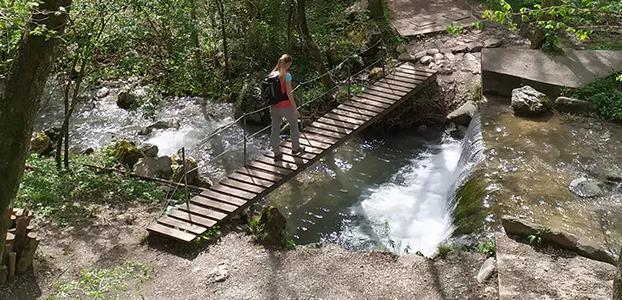
\includegraphics[width=\linewidth, height=5.2cm, keepaspectratio]{ponte_artigianale}\\[4pt]
  \begin{tcolorbox}[colback=swlight, colframe=swgray, boxrule=0.5pt, arc=2pt, width=\linewidth]
  \small\textbf{Passerella in legno}\\
  1 artigiano, 10 giorni, circa 5.000\,€.\\
  Un approccio \textbf{non strutturato} è sufficiente.
  \end{tcolorbox}
\end{minipage}\hfill
\begin{minipage}[t]{0.47\textwidth}
  \centering
  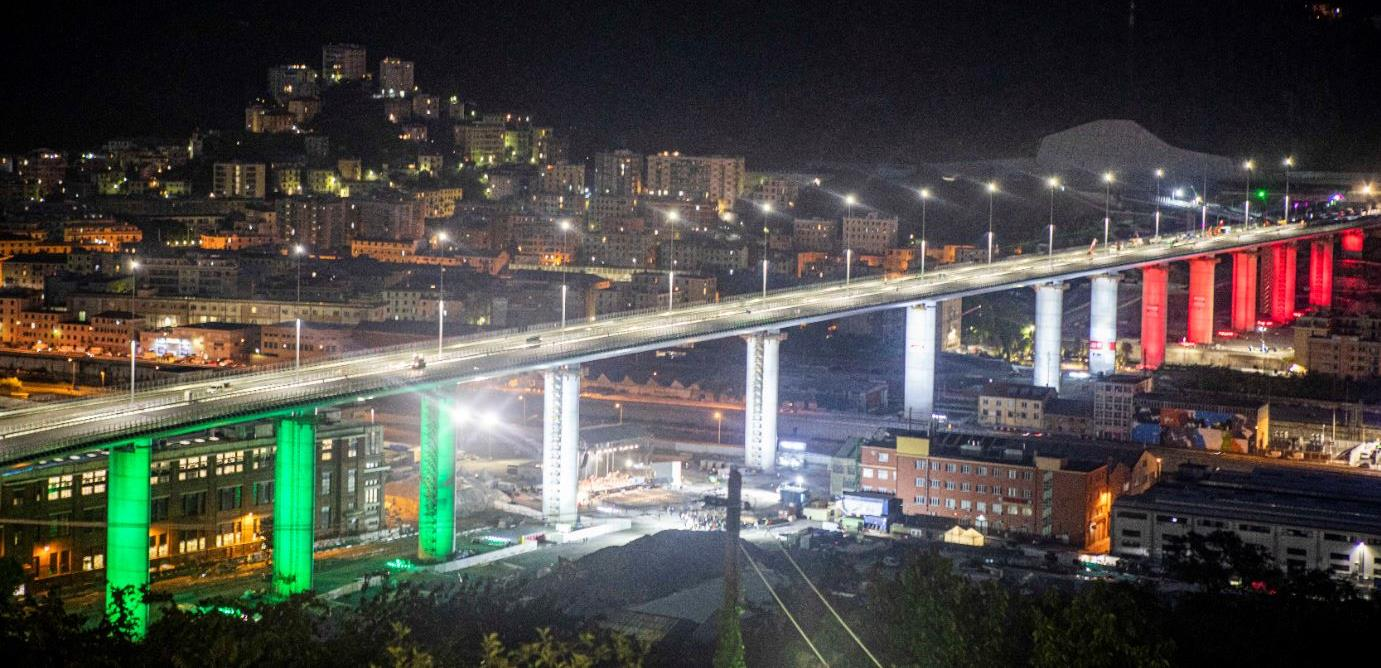
\includegraphics[width=\linewidth, height=5.2cm, keepaspectratio]{ponte_san_giorgio_notte}\\[4pt]
  \begin{tcolorbox}[colback=swlight, colframe=swblue, boxrule=0.5pt, arc=2pt, width=\linewidth]
  \small\textbf{Viadotto San Giorgio (Genova)}\\
  1.000 persone, 330 aziende coinvolte.\\
  Serve un approccio \textbf{sistematico e strutturato}.
  \end{tcolorbox}
\end{minipage}
\caption{Stessa funzione (attraversare), complessità incomparabili.}
\end{figure}

Entrambi sono «ponti», ma nessuno costruirebbe un viadotto autostradale come si costruisce una passerella nel bosco:
servono progettisti, calcoli, normative, collaudi, coordinamento tra centinaia di persone.
Con il software succede esattamente la stessa cosa: un programmino da 200 righe si può scrivere «di getto»,
un sistema bancario da milioni di righe no.

\info{L'idea chiave}{
  L'\textbf{ingegneria} entra in gioco quando la complessità del problema supera la capacità di un singolo individuo di
  tenerlo sotto controllo. A quel punto l'improvvisazione non basta più: servono \textbf{metodi, processi e strumenti}.
}

% ============================================================
\section{Un po' di storia}

\begin{minipage}[t]{0.60\textwidth}
\vspace{0pt}
\subsection{Gli inizi: l'hardware è il protagonista}

Nel 1946 viene presentato l'\textbf{ENIAC} (\textit{Electronic Numerical Integrator and Computer}), uno dei primi calcolatori elettronici programmabili.
In quegli anni:
\begin{itemize}
  \item i calcolatori erano macchine enormi, costosissime e sbalorditive;
  \item la macchina era molto più «spettacolare» (e costosa) di qualche foglio di codice;
  \item la programmazione era considerata un'attività \textbf{secondaria} rispetto all'ingegneria dell'hardware;
  \item i programmi venivano sviluppati per lo più \textbf{individualmente}, spesso da chi poi li usava.
\end{itemize}
\end{minipage}\hfill
\begin{minipage}[t]{0.37\textwidth}
\vspace{0pt}
\centering
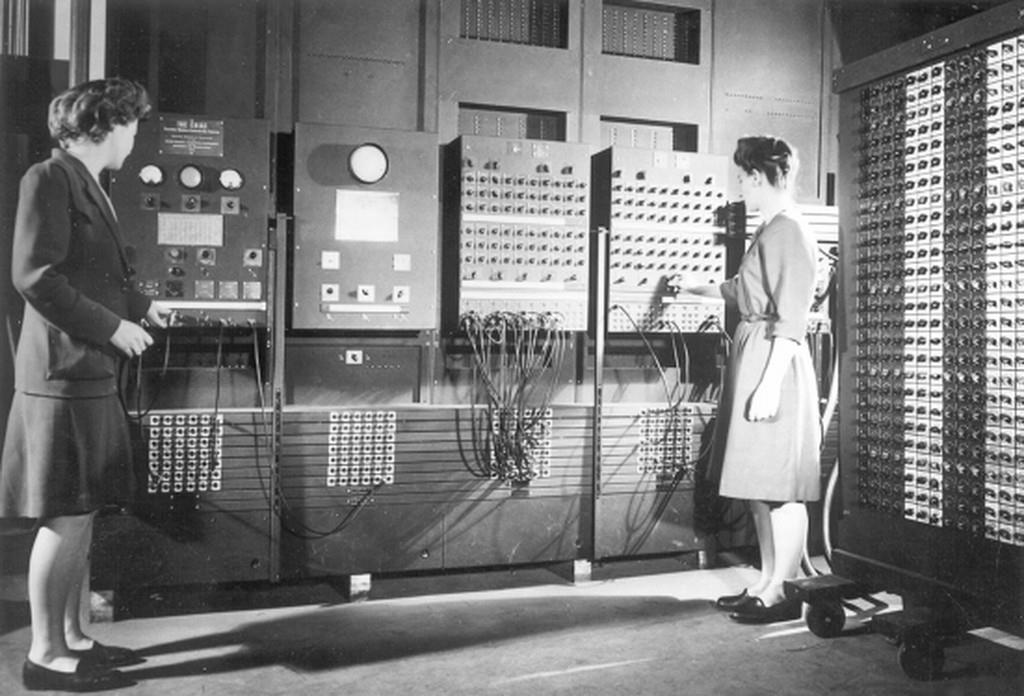
\includegraphics[width=\linewidth]{eniac}\\[2pt]
{\scriptsize Jean Bartik (a sinistra) e Frances Spence al lavoro sull'ENIAC.}
\end{minipage}

\begin{minipage}[t]{0.30\textwidth}
\vspace{0pt}
\centering
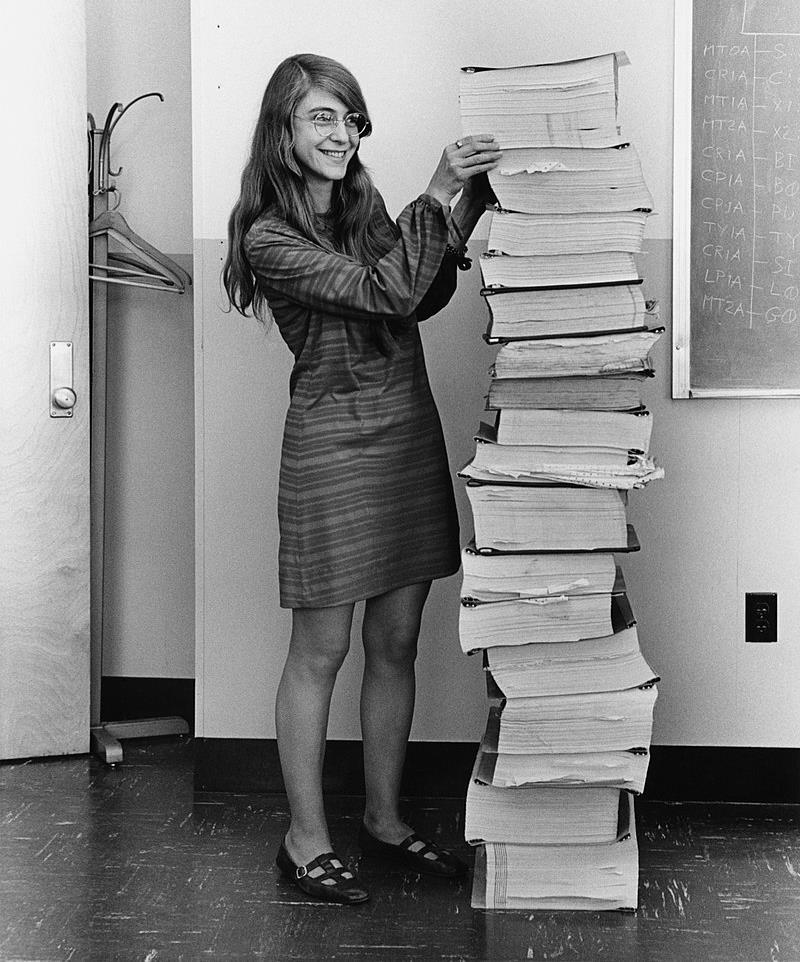
\includegraphics[width=0.95\linewidth]{margaret_hamilton}\\[2pt]
{\scriptsize Margaret Hamilton nel 1969, accanto al codice scritto dal suo team per l'Apollo Guidance Computer.}
\end{minipage}\hfill
\begin{minipage}[t]{0.66\textwidth}
\vspace{0pt}
\subsection{Anni '60: la crisi del software}

Negli anni '60 i sistemi diventano molto più complessi (si pensi ai programmi spaziali della NASA).
Gli approcci individuali \textbf{non scalano}: quello che funziona per un programma piccolo crolla su sistemi grandi.

Nasce così la cosiddetta \hi{crisi del software}: i sistemi erano
\begin{itemize}
  \item \textbf{inaffidabili} (pieni di errori);
  \item \textbf{fuori budget} (costavano molto più del previsto);
  \item \textbf{in ritardo} rispetto ai tempi di consegna pianificati.
\end{itemize}

Diventa evidente il bisogno di una nuova disciplina che studi \textbf{metodologie per la produzione del software}.
Il termine \textit{software engineering} si diffonde in quegli anni: fu usato da Margaret Hamilton,
che guidava il team del software di bordo delle missioni Apollo, e diede il titolo a una famosa conferenza NATO del 1968
dedicata proprio alla crisi del software.
\end{minipage}

% ============================================================
\section{L'approccio ingenuo}

L'approccio con cui abbiamo lavorato finora nei corsi di programmazione è più o meno questo:

\begin{center}
\begin{tikzpicture}
  \node[card=swteal, minimum width=3.2cm, minimum height=1.1cm] (req) {\textbf{Requisiti}\\\scriptsize(la traccia)};
  \node[single arrow, draw=swgray, fill=swgray!20, minimum height=3.4cm, minimum width=1.2cm, single arrow head extend=2mm, right=0.4cm of req, font=\small] (cod) {coding};
  \node[card=swteal, minimum width=3.2cm, minimum height=1.1cm, right=0.4cm of cod] (prog) {\textbf{Programma}};
  \node[font=\Large\bfseries, text=swred] at ([yshift=0.9cm]req.north) {?};
  \node[font=\Large\bfseries, text=swred] at ([yshift=0.9cm]cod.north) {?};
  \node[font=\Large\bfseries, text=swred] at ([yshift=0.9cm]prog.north) {?};
\end{tikzpicture}
\end{center}

Leggiamo la traccia, scriviamo il codice, otteniamo il programma. Funziona benissimo per un esercizio d'esame,
ma appena il problema diventa reale emergono subito delle domande a cui questo schema non sa rispondere:

\begin{table}[H]
\centering
\renewcommand{\arraystretch}{1.35}
\begin{tabularx}{\textwidth}{>{\bfseries}P{3.9cm} L}
\toprule
Aspetto & Domande senza risposta \\
\midrule
Requisiti & Da dove arrivano? Sono corretti? Sono completi? Il cliente sa davvero cosa vuole? \\
Organizzazione & Come strutturo il programma? In quali moduli e classi lo divido? \\
Lavoro in team & Come divido il lavoro tra più programmatori? Come ci coordiniamo? \\
Correttezza & I requisiti sono davvero soddisfatti? Come faccio a sapere che il programma è corretto? \\
Cambiamento & Cosa succede quando i requisiti cambiano a metà strada (e cambieranno)? \\
\bottomrule
\end{tabularx}
\end{table}

L'Ingegneria del Software esiste proprio per dare una risposta \textbf{sistematica} a ciascuna di queste domande.

% ============================================================
\section{La dimensione conta}

Qual è il programma più grande che abbiamo mai scritto? E prima ancora: \textbf{come si misura la «dimensione» di un software?}
Una misura semplice (anche se imperfetta) sono le \hi{LOC} (\textit{Lines Of Code}), cioè le righe di codice,
di solito contate escludendo commenti e righe vuote.

Un progetto medio del corso di Programmazione a Oggetti dello scorso anno contava circa \textbf{3.000 righe} di codice
non di commento (incluse quelle generate automaticamente) e circa \textbf{35 classi}. Sembra tanto lavoro, vero?
Confrontiamolo con alcuni sistemi reali:

\begin{figure}[H]
\centering
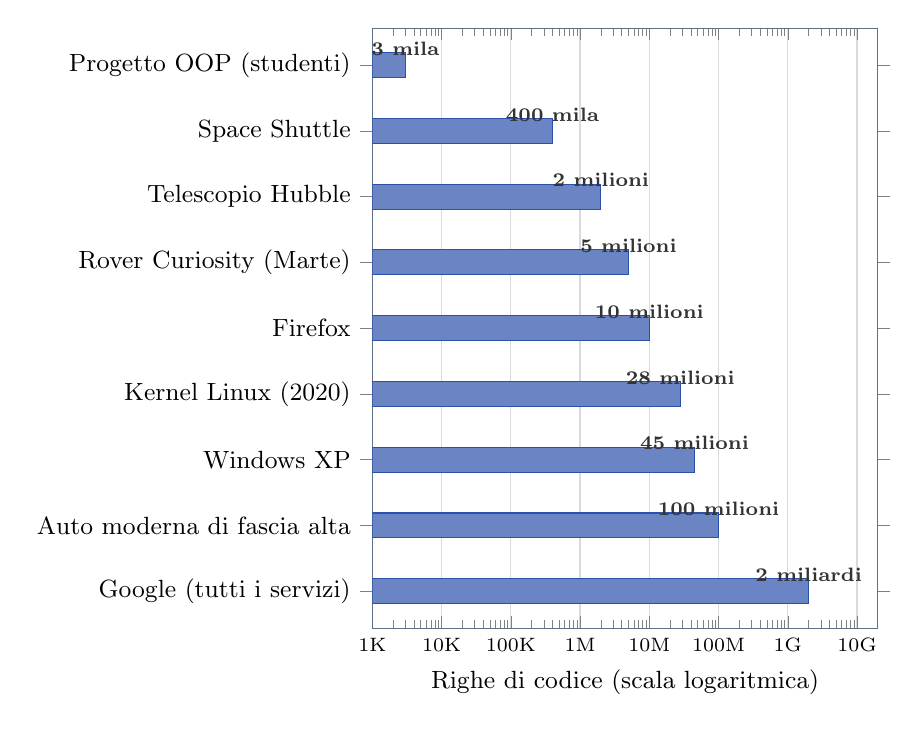
\begin{tikzpicture}
\begin{axis}[
  xbar, xmode=log, log origin=infty,
  width=0.66\textwidth, height=9.2cm,
  xmin=1000, xmax=2e10,
  bar width=9pt,
  y dir=reverse,
  ytick={1,...,9},
  yticklabels={{Progetto OOP (studenti)},{Space Shuttle},{Telescopio Hubble},{Rover Curiosity (Marte)},{Firefox},{Kernel Linux (2020)},{Windows XP},{Auto moderna di fascia alta},{Google (tutti i servizi)}},
  yticklabel style={font=\small},
  xlabel={Righe di codice (scala logaritmica)},
  xlabel style={font=\small},
  xtick={1e3,1e4,1e5,1e6,1e7,1e8,1e9,1e10},
  xticklabels={1K,10K,100K,1M,10M,100M,1G,10G},
  xticklabel style={font=\scriptsize},
  xmajorgrids, grid style={swgray!25},
  axis line style={swgray},
  nodes near coords, point meta=explicit symbolic,
  every node near coord/.append style={font=\scriptsize\bfseries, text=black!80},
  enlarge y limits=0.07,
]
\addplot[fill=swblue!70, draw=swblue] coordinates {
  (3000,1) [3 mila]
  (400000,2) [400 mila]
  (2000000,3) [2 milioni]
  (5000000,4) [5 milioni]
  (10000000,5) [10 milioni]
  (28000000,6) [28 milioni]
  (45000000,7) [45 milioni]
  (100000000,8) [100 milioni]
  (2000000000,9) [2 miliardi]
};
\end{axis}
\end{tikzpicture}
\caption{Ordini di grandezza del software reale (stime diffuse pubblicamente, arrotondate).}
\end{figure}

\warning{Attenzione alla scala}{
  L'asse orizzontale è \textbf{logaritmico}: ogni tacca vale 10 volte la precedente. Il progetto di OOP è quindi più piccolo
  di un fattore 100 rispetto al software dello Space Shuttle, e di quasi un milione di volte rispetto all'insieme dei servizi Google.
  A queste dimensioni nessuna persona può conoscere tutto il codice: \textbf{servono metodo e organizzazione}.
}

% ============================================================
\section{Programmi e prodotti software}

Una distinzione fondamentale è quella tra \textbf{programma} e \textbf{prodotto software}.

\dfn{Programma}{
  Software sviluppato generalmente da \textbf{una sola persona}, che spesso ne è anche l'utente principale.
  Non richiede un processo formale né documentazione e in genere non è commercializzabile.
}

\dfn{Prodotto software}{
  Software sviluppato da \textbf{team} e usato da \textbf{altre persone}. È un prodotto industriale, sviluppato e testato secondo
  standard, che comprende molto più del solo codice sorgente o dell'eseguibile e che deve \textbf{evolvere nel tempo}.
}

\begin{table}[H]
\centering
\renewcommand{\arraystretch}{1.35}
\begin{tabularx}{\textwidth}{>{\bfseries}P{3.3cm} L L}
\toprule
 & \textcolor{swteal}{Programma} & \textcolor{swblue}{Prodotto software} \\
\midrule
Chi lo sviluppa & Una persona & Uno o più team \\
Chi lo usa & Lo sviluppatore stesso & Altre persone (clienti, utenti finali) \\
Processo & Nessun processo formale & Processo strutturato e documentato \\
Costi & Bassi & Significativamente più alti \\
Cosa comprende & Codice (ed eseguibile) & Codice, documentazione, manuali utente, manuali di installazione e configurazione, suite di test automatici \\
Ciclo di vita & «Usa e getta», one-shot & Evolve nel tempo (versioni, aggiornamenti, correzioni) \\
Esempio & Uno script per rinominare le foto delle vacanze & Un'app di home banking \\
\bottomrule
\end{tabularx}
\caption{Programma e prodotto software a confronto.}
\end{table}

\subsection{Tipi di prodotti software}

I prodotti software si dividono in due grandi famiglie. La differenza chiave è \textbf{chi definisce i requisiti}.

\begin{figure}[H]
\centering
\begin{tikzpicture}
  % --- Riga 1: software generico
  \node[chip=swblue, minimum width=17.5cm, minimum height=0.75cm, font=\small\bfseries, anchor=west] at (0,0) {Software generico (\textit{off-the-shelf})};
  \node[card=swblue, minimum width=2.4cm, minimum height=1.1cm] (mk) at (1.4,-1.7) {Team di\\marketing};
  \node[card=swblue, minimum width=2.4cm, minimum height=1.1cm] (p1) at (5.2,-1.7) {Prodotto\\generico};
  \draw[flow] (mk) -- node[above, font=\scriptsize]{requisiti} (p1);
  \foreach \k/\dy in {1/0.55,2/0,3/-0.55}{
    \node[font=\scriptsize, anchor=west] (u\k) at (7.6,-1.7+\dy) {\iuser\ cliente \k};
    \draw[-{Stealth}, swgray] (p1.east) -- (u\k.west);
  }
  \node[note, anchor=west, text width=7.6cm] at (9.7,-1.7) {Pensato per un \textbf{mercato}: venduto o distribuito a chiunque sia interessato.\\[2pt]\textit{Esempi}: Microsoft Office, Photoshop, Firefox, un videogioco.};

  % --- Riga 2: software su commessa
  \node[chip=sworange, minimum width=17.5cm, minimum height=0.75cm, font=\small\bfseries, anchor=west] at (0,-3.4) {Software su commessa (\textit{customly-developed})};
  \node[card=sworange, minimum width=2.4cm, minimum height=1.1cm] (cl) at (1.4,-5.1) {\iuser\ Cliente};
  \node[card=sworange, minimum width=2.4cm, minimum height=1.1cm] (p2) at (5.2,-5.1) {Prodotto\\su misura};
  \draw[flow] ([yshift=2mm]cl.east) -- node[above, font=\scriptsize]{requisiti} ([yshift=2mm]p2.west);
  \draw[flow, sworange] ([yshift=-3mm]p2.west) -- node[below, font=\scriptsize]{consegna} ([yshift=-3mm]cl.east);
  \node[note, anchor=west, text width=7.6cm] at (9.7,-5.1) {Sviluppato per le \textbf{esigenze specifiche} di un committente, che definisce i requisiti.\\[2pt]\textit{Esempi}: il gestionale di un ospedale, il sistema paghe di un ente pubblico.};
\end{tikzpicture}
\caption{La differenza chiave: chi definisce i requisiti (il marketing o il cliente).}
\end{figure}

\begin{esercizio}{Programma o prodotto? Generico o su commessa?}
Classifica i seguenti casi.
\begin{enumerate}
  \item Uno script Python che uno studente usa per calcolare la media dei propri voti.
  \item Il sistema di prenotazione degli esami realizzato per un'università.
  \item Un videogioco venduto su una piattaforma di distribuzione digitale.
  \item Il software di gestione del magazzino commissionato da una catena di supermercati.
\end{enumerate}

\textbf{Soluzione.}
(1) \textit{Programma}: una persona, un utente, nessun processo.
(2) \textit{Prodotto su commessa}: i requisiti li detta l'università.
(3) \textit{Prodotto generico}: i requisiti li definisce l'azienda (marketing) pensando a un mercato.
(4) \textit{Prodotto su commessa}.
\end{esercizio}

% ============================================================
\section{Lo sviluppo professionale}

Lo sviluppo professionale del software non è (solo) un'\textbf{arte} artigianale né (solo) una \textbf{scienza}: è un \hi{processo industriale}.
\begin{itemize}
  \item Il software viene sviluppato da \textbf{aziende}, organizzate in \textbf{team} con molti membri.
  \item Si lavora con \textbf{vincoli di tempo e di costo} e con \textbf{requisiti di qualità} stringenti.
  \item Come per ogni processo industriale, sono state sviluppate \textbf{metodologie} che guidano progettazione, sviluppo e verifica.
        Queste metodologie non nascono dal nulla: \textbf{formalizzano l'esperienza} accumulata in decenni di progetti (riusciti e falliti).
\end{itemize}

\warning{Essere il miglior programmatore non basta}{
  Da professionisti dell'informatica queste metodologie vanno \textbf{conosciute}. Un ottimo programmatore che non sa lavorare
  dentro un processo, in un team, con un cliente, produrrà comunque software di scarsa qualità.
}

% ============================================================
\section{Cos'è l'Ingegneria del Software}

Esistono diverse definizioni, che guardano la disciplina da punti di vista leggermente diversi.

\dfn{Ingegneria del Software (Sommerville)}{
  È la \textbf{disciplina ingegneristica} che si occupa di \textbf{tutti gli aspetti} della produzione di software professionale.
}

Analizziamo le due parti in grassetto:
\begin{itemize}
  \item \textbf{Disciplina ingegneristica}: gli ingegneri \textit{fanno funzionare le cose}. Applicano teorie, metodi e strumenti
        \textbf{dove sono appropriati}, per risolvere problemi rispettando i vincoli organizzativi ed economici. Non si cerca la soluzione
        «perfetta» in astratto, ma quella migliore \textit{date le risorse disponibili}.
  \item \textbf{Tutti gli aspetti della produzione}: non solo la programmazione! Rientrano anche la \textbf{gestione del progetto}
        (pianificazione, persone, costi) e lo sviluppo di strumenti, metodi e teorie a supporto dello sviluppo.
\end{itemize}

\dfn{Ingegneria del Software (IEEE)}{
  È l'applicazione di un approccio \textbf{sistematico, disciplinato e quantificabile} allo sviluppo, all'esercizio e alla manutenzione
  del software; in altre parole, l'applicazione dell'ingegneria al software.
}

\dfn{Ingegneria del Software (Bruegge e Dutoit)}{
  È lo stato dell'arte dello sviluppo di \textbf{software di qualità}, \textbf{nei tempi} e \textbf{nei costi} previsti.
}

\info{Cosa hanno in comune le definizioni}{
  Tutte e tre sottolineano che non basta «far funzionare il codice»: conta \textbf{come} ci si arriva (in modo sistematico),
  \textbf{cosa} si ottiene (qualità) e \textbf{a quali condizioni} (tempo e budget). Inoltre il lavoro non finisce con la consegna:
  esercizio e manutenzione fanno parte della disciplina.
}

% ============================================================
\section{Perché è difficile}

Produrre software di alta qualità rispettando budget e vincoli organizzativi \textbf{non è facile}. I motivi principali sono tre.

\begin{center}
\begin{tikzpicture}
  \node[card=swblue, text width=5.3cm, minimum height=3.7cm, align=left] (a) {%
    \textbf{\large 1. È astratto e intangibile}\\[4pt]
    \small Non è vincolato dalle proprietà dei materiali o dalle leggi della fisica. Per questo può diventare
    \textbf{estremamente complesso} molto in fretta, senza che nessuno «veda» il problema.};
  \node[card=sworange, text width=5.3cm, minimum height=3.7cm, align=left, right=0.35cm of a] (b) {%
    \textbf{\large 2. È ovunque ed è diverso}\\[4pt]
    \small Infrastrutture nazionali, elettrodomestici, industria, finanza, intrattenimento\ldots\
    Ogni dominio ha esigenze molto diverse dagli altri.};
  \node[card=swred, text width=5.3cm, minimum height=3.7cm, align=left, right=0.35cm of b] (c) {%
    \textbf{\large 3. Non esiste un metodo universale}\\[4pt]
    \small Nessuna metodologia va bene per ogni tipo di software, azienda e situazione.
    E nessuna tecnologia è una \textbf{pallottola d'argento} che risolve tutto.};
\end{tikzpicture}
\end{center}

\info{No Silver Bullet}{
  L'espressione «pallottola d'argento» viene dal celebre articolo \textit{No Silver Bullet} di Fred Brooks (1986):
  come nelle leggende solo una pallottola d'argento uccide il lupo mannaro, così si sperava in una tecnologia capace di
  eliminare da sola la complessità del software. Brooks sosteneva che \textbf{non esiste}: la complessità è in buona parte
  \textit{essenziale}, cioè intrinseca al problema, e nessuno strumento può farla sparire.
}

\subsection{Progetti che sono andati male}

Ancora oggi i progetti software falliscono o incontrano problemi seri: sforano il budget, sforano i tempi di rilascio,
consegnano un prodotto che non rispetta i requisiti di qualità\ldots\ o che non funziona affatto.

\begin{table}[H]
\centering
\renewcommand{\arraystretch}{1.4}
\begin{tabularx}{\textwidth}{>{\bfseries}P{3.4cm} L >{\centering\arraybackslash}p{3.2cm}}
\toprule
Progetto & Cosa è successo & Costo \\
\midrule
Healthcare.gov (USA) & Portale sanitario commissionato dal governo federale. Nella prima settimana solo l'1\% degli utenti riuscì a iscriversi. & \textbf{1,5 mld \$}\newline\scriptsize(15 volte i 93,7 mln previsti) \\
Queensland Health (Australia) & Nuovo sistema paghe per 80.000 dipendenti di 16 dipartimenti. Avviato nel 2007 con rilascio previsto nel 2008: rilasciato nel 2010, funzionava a malapena, sistemato solo nel 2018. & \textbf{$\sim$850 mln \$}\newline\scriptsize(200 volte i 4,2 mln previsti) \\
Cyberpunk 2077 & Videogioco annunciato nel 2012, uscita prevista ad aprile 2020, rinviata più volte fino a dicembre 2020. Al rilascio era pieno di bug e ingiocabile su alcune console. & \textbf{$\sim$400 mln \$} \\
\midrule
\rowcolor{swlight} Per confronto: Viadotto San Giorgio & 1,1 km di lunghezza, 45 m di altezza, 4 corsie + 2 di emergenza. Costruito in circa \textbf{un anno}. & \textbf{202 mln €} \\
\bottomrule
\end{tabularx}
\caption{Alcuni progetti software problematici, confrontati con un'opera di ingegneria civile.}
\end{table}

Il confronto è impietoso: un viadotto autostradale è costato meno di molti sistemi informativi falliti.
L'ingegneria civile ha secoli di esperienza e metodi consolidati; l'ingegneria del software è molto più giovane.

\subsection{Quando i problemi non sono solo economici}

A volte le conseguenze di un software difettoso vanno ben oltre il budget:

\begin{itemize}
  \item \textbf{London Ambulance Service (1992)}: il nuovo sistema computerizzato di smistamento delle ambulanze andò in crisi poco dopo l'avvio,
        causando enormi ritardi nei soccorsi; ai disservizi furono attribuiti numerosi decessi.
  \item \textbf{Ariane 5, volo 501 (1996)}: il razzo europeo si autodistrusse circa 40 secondi dopo il lancio. Un modulo software riusato
        dall'Ariane 4 convertiva un numero in virgola mobile a 64 bit in un intero a 16 bit: con le traiettorie più veloci del nuovo razzo
        il valore non ci stava più (\textit{overflow}).
  \item \textbf{Boeing 737 MAX (2018--2019)}: due incidenti con 346 vittime complessive, legati al sistema automatico di controllo MCAS,
        che si basava sui dati di un singolo sensore.
\end{itemize}

\error{Il messaggio}{
  Il software controlla ospedali, aerei, centrali, banche. Un difetto di \textbf{processo} (requisiti sbagliati, test insufficienti,
  riuso senza verifica, cattiva comunicazione) può costare vite umane. Per questo servono metodi ingegneristici.
}

% ============================================================
\section{Il lavoro dell'ingegnere del software}

Riassumendo, un ingegnere del software deve:
\begin{itemize}
  \item adottare un approccio \textbf{sistematico e organizzato} alla produzione del software;
  \item usare \textbf{strumenti, tecniche e metodologie appropriati}, scelti in base al problema da risolvere,
        ai vincoli di sviluppo e organizzativi e alle risorse disponibili;
\end{itemize}
per produrre \textbf{software di alta qualità}\ldots
\begin{center}
\begin{tikzpicture}
  \coordinate (Q) at (0,3.1);
  \coordinate (B) at (-3.3,0);
  \coordinate (T) at (3.3,0);
  \fill[swblue!8] (Q) -- (B) -- (T) -- cycle;
  \draw[line width=1.4pt, swblue] (Q) -- (B) -- (T) -- cycle;
  \node[chip=swblue, font=\small\bfseries, minimum width=2.6cm] at (Q) {Alta qualità};
  \node[chip=sworange, font=\small\bfseries, minimum width=2.6cm] at (B) {\ldots entro il budget};
  \node[chip=swred, font=\small\bfseries, minimum width=2.6cm] at (T) {\ldots entro la scadenza};
  \node[font=\small\itshape, text=swgray, align=center] at (0,1.05) {\ldots mentre\\i requisiti cambiano!};
  \draw[decorate, decoration={snake, amplitude=1.2pt, segment length=7pt}, swgray, line width=0.8pt, -{Stealth}]
     (-4.8,1.6) -- node[above, font=\scriptsize, sloped]{cambiamenti} (-2.1,1.6);
  \draw[decorate, decoration={snake, amplitude=1.2pt, segment length=7pt}, swgray, line width=0.8pt, -{Stealth}]
     (4.8,1.6) -- node[above, font=\scriptsize, sloped]{cambiamenti} (2.1,1.6);
\end{tikzpicture}
\end{center}

\gbox{In sintesi}{azure-gradient-6!80!black}{
\begin{itemize}
  \item L'Ingegneria del Software nasce dalla \textbf{crisi del software} degli anni '60: gli approcci individuali non scalano.
  \item Un \textbf{prodotto software} non è un programma: è sviluppato da team, per altri, include documentazione e test, ed evolve.
  \item Il software è \textbf{difficile} da ingegnerizzare: intangibile, ovunque, senza metodi universali.
  \item L'obiettivo è produrre \textbf{qualità} rispettando \textbf{tempi} e \textbf{costi}, gestendo il \textbf{cambiamento}.
\end{itemize}
}


  \chapter{I processi software}

\section{Cos'è un processo software}

Nel capitolo precedente abbiamo visto che serve un approccio \textbf{sistematico} alla produzione del software.
Il primo strumento per ottenerlo è il concetto di \textit{processo}.

\dfn{Processo software}{
  Un \textbf{processo software} è un insieme di \textbf{attività correlate} che porta alla produzione di un sistema software.
}

Un'analogia utile è la costruzione di una casa: non si comincia posando mattoni a caso, ma si segue una sequenza
di attività (capire le esigenze di chi ci abiterà, fare il progetto, ottenere i permessi, costruire, collaudare, fare manutenzione).
Il processo software è l'equivalente per il software: stabilisce \textbf{quali attività} svolgere, \textbf{in che ordine},
\textbf{chi} le svolge e \textbf{cosa} producono.

\warning{Non esiste il processo perfetto}{
  Non esiste un processo universale che funzioni sempre. Esistono (e si usano) \textbf{molti processi diversi}, e ognuno va
  \textbf{adattato alla situazione}: al tipo di software, all'azienda, al cliente, al team.
}

Per capire perché, basta confrontare due progetti molto diversi:

\begin{table}[H]
\centering
\renewcommand{\arraystretch}{1.4}
\begin{tabularx}{\textwidth}{>{\bfseries}P{4cm} L L}
\toprule
 & \textcolor{swred}{Software di un pacemaker} & \textcolor{swblue}{App di una startup} \\
\midrule
Conseguenze di un errore & Possono essere letali & Utenti insoddisfatti, perdita di clienti \\
Stabilità dei requisiti & Molto stabili, fissati da normative & Cambiano di settimana in settimana \\
Documentazione & Estesa e obbligatoria (certificazioni) & Ridotta al minimo indispensabile \\
Priorità & Sicurezza e correttezza & Velocità di rilascio e feedback \\
Processo adatto & Rigoroso, pianificato, molto controllato & Leggero, iterativo, flessibile \\
\bottomrule
\end{tabularx}
\caption{Contesti diversi richiedono processi diversi.}
\end{table}

% ============================================================
\section{Le quattro attività fondamentali}

Per quanto i processi possano essere diversi tra loro, \textbf{tutti} includono, in qualche forma, quattro attività fondamentali.

\begin{figure}[H]
\centering
\begin{tikzpicture}
  \foreach \i/\titolo/\col/\desc in {
      0/{Software\\Specification}/swteal/{Si definiscono le \textbf{funzionalità} e i \textbf{vincoli operativi} del software.},
      1/{Software\\Implementation}/swblue/{Si \textbf{produce} il software che soddisfa i requisiti.},
      2/{Software\\Validation}/ph3/{Si \textbf{verifica} che il software soddisfi i requisiti.},
      3/{Software\\Evolution}/ph6/{Il software \textbf{evolve} per rispondere a esigenze che cambiano.}}{
    \node[phase=\col, minimum width=3.4cm, minimum height=1.3cm, font=\small\bfseries, drop shadow] (a\i) at (\i*4.55,0) {\titolo};
    \node[note, text width=3.5cm, align=center, font=\small, anchor=north] at (\i*4.55,-0.9) {\desc};
  }
  \foreach \i [evaluate=\i as \j using int(\i+1)] in {0,1,2}{
    \node[single arrow, fill=swgray!40, draw=none, minimum height=0.9cm, minimum width=0.7cm, single arrow head extend=1.5mm, inner sep=0pt] at ($(a\i.east)!0.5!(a\j.west)$) {};
  }
\end{tikzpicture}
\caption{Le quattro attività fondamentali presenti in ogni processo software.}
\end{figure}

\subsection{Software Specification (specifica)}

È l'attività in cui si stabilisce \textbf{cosa} il sistema deve fare e \textbf{sotto quali vincoli} deve operare.
Si parla con il cliente e con gli utenti, si analizza il dominio del problema e si mettono per iscritto i requisiti.

\begin{esempio}{Specifica di un sistema per la prenotazione degli esami}
  \textit{Funzionalità}: lo studente può vedere gli appelli disponibili, prenotarsi e cancellare la prenotazione.\\
  \textit{Vincoli operativi}: il sistema deve gestire 5.000 prenotazioni contemporanee nel giorno di apertura degli appelli
  e deve essere accessibile anche da smartphone.
\end{esempio}

\subsection{Software Implementation (sviluppo)}

È l'attività in cui si \textbf{produce} il software che soddisfa la specifica. Attenzione: nonostante il nome, non si tratta
solo di scrivere codice. L'implementazione in senso ampio comprende la \textbf{progettazione} (come organizzare il sistema)
e la \textbf{programmazione} vera e propria. In alcuni testi questa attività è infatti chiamata \textit{Software Development}.

\subsection{Software Validation (validazione)}

Il software prodotto va \textbf{controllato}: bisogna assicurarsi che faccia quello che la specifica richiede
e che risponda alle aspettative del cliente. Questo avviene principalmente tramite revisioni e \textbf{test}.

\subsection{Software Evolution (evoluzione)}

Il software \textbf{non è mai «finito»}. Una volta in uso deve cambiare per rispondere a esigenze che cambiano. Alcuni esempi tipici:
\begin{itemize}
  \item esce una \textbf{nuova versione del sistema operativo} e l'applicazione va adattata;
  \item viene scoperto un \textbf{bug} sfuggito ai test;
  \item entra in vigore una \textbf{nuova legge} che cambia le procedure (es.\ un nuovo calcolo delle tasse);
  \item il cliente chiede \textbf{nuove funzionalità}.
\end{itemize}

\info{{Attività complesse, fatte da persone}}{
  \begin{itemize}
    \item Queste attività sono \textbf{complesse} e ciascuna comprende molte \textbf{sotto-attività} (le vedremo nel modello a cascata).
    \item Come ogni processo creativo, i processi software si basano su \textbf{persone} che prendono \textbf{decisioni} ed esprimono \textbf{giudizi}:
          nessun processo può essere eseguito «meccanicamente».
    \item Oltre alle quattro attività principali, un processo include tipicamente \textbf{attività di supporto}, come la
          \textbf{pianificazione} del progetto e il suo \textbf{monitoraggio} (stiamo rispettando tempi e costi?).
  \end{itemize}
}

\begin{figure}[H]
\centering
\begin{tikzpicture}
  \foreach \i/\titolo/\col in {0/Specifica/swteal, 1/Implementazione/swblue, 2/Validazione/ph3, 3/Evoluzione/ph6}{
    \node[phase=\col, minimum width=3.6cm, minimum height=0.9cm, font=\small\bfseries] (b\i) at (\i*4.1,0) {\titolo};
  }
  \node[fit=(b0)(b3), draw=swgray, dashed, rounded corners=4pt, inner sep=6pt, label={[font=\scriptsize\bfseries, text=swgray]above:Attività fondamentali}] (fund) {};
  \node[rectangle, rounded corners=3pt, fill=swgray!15, draw=swgray!60, minimum width=16.1cm, minimum height=0.8cm, font=\small, below=0.35cm of fund] (supp) {\textbf{Attività di supporto}: pianificazione del progetto, monitoraggio di tempi e costi, \ldots};
  \node[font=\small\itshape, text=swgray, below=0.15cm of supp] {\iuser\ \iuser\ \iuser\quad svolte da persone che prendono decisioni e giudizi\quad\iuser\ \iuser\ \iuser};
\end{tikzpicture}
\caption{Le attività di supporto accompagnano per tutta la durata le attività fondamentali.}
\end{figure}

% ============================================================
\section{Il ciclo di vita del software}

Le quattro attività fondamentali, ripetute nel tempo, descrivono il \hi{ciclo di vita} del software.
Si parla di «ciclo» perché l'evoluzione riporta continuamente a nuove specifiche: ogni modifica richiede di capire
cosa cambiare, implementarlo, validarlo e rilasciarlo.

\begin{figure}[H]
\centering
\begin{tikzpicture}
  \def\R{2.6}
  \node[circle, fill=primary!10, draw=primary!60, minimum size=2.9cm, align=center, font=\small\bfseries, text=primary!80!black] (c) at (0,0) {Ciclo di vita\\del software};
  \node[phase=swteal, minimum width=3.1cm] (s) at (90:\R) {Specifica};
  \node[phase=swblue, minimum width=3.1cm] (i) at (0:\R+1.6) {Implementazione};
  \node[phase=ph3, minimum width=3.1cm] (v) at (270:\R) {Validazione};
  \node[phase=ph6, minimum width=3.1cm] (e) at (180:\R+1.6) {Evoluzione};
  \draw[flow, line width=1.5pt, swgray!80] (s.east) to[out=0, in=90] (i.north);
  \draw[flow, line width=1.5pt, swgray!80] (i.south) to[out=270, in=0] (v.east);
  \draw[flow, line width=1.5pt, swgray!80] (v.west) to[out=180, in=270] (e.south);
  \draw[flow, line width=1.5pt, swred] (e.north) to[out=90, in=180] node[above left, font=\scriptsize, text=swred, align=right]{nuove esigenze,\\nuovi requisiti} (s.west);

  % Nascita e morte
  \node[card=swgreen, font=\scriptsize, text width=3.2cm, align=left] (nasc) at (7.6,2.1) {\textbf{Nascita}: qualcuno \textbf{richiede} il software (un cliente o il mercato).};
  \node[card=swred, font=\scriptsize, text width=3.2cm, align=left] (mor) at (7.6,-2.1) {\textbf{Morte}: esplicita attività di \textbf{dismissione}, ad esempio quando viene sostituito da un altro software.};
  \draw[-{Stealth}, swgreen, line width=1pt, dashed] (nasc.west) to[out=180, in=20] (s.east);
  \draw[-{Stealth}, swred, line width=1pt, dashed] (e.south west) to[out=240, in=180] ([yshift=-1.0cm]v.south) -- ([yshift=-1.0cm]v.south -| mor.west) -- ([yshift=-0.2cm]mor.west);
\end{tikzpicture}
\caption{Il ciclo di vita: dalla richiesta iniziale fino alla dismissione.}
\end{figure}

\dfn{Nascita e morte del software}{
  La vita di un software \textbf{inizia} quando qualcuno ne fa richiesta e \textbf{termina} solo con un'esplicita
  \textbf{attività di dismissione} (ad esempio quando va sostituito con un altro sistema). Tra questi due estremi il software
  attraversa ripetutamente le attività di specifica, implementazione, validazione ed evoluzione.
}

Un aspetto spesso sottovalutato è \textbf{quanto} dura questa vita. Lo sviluppo iniziale può durare mesi,
ma l'esercizio e la manutenzione possono durare \textbf{anni o decenni}: molte banche e pubbliche amministrazioni usano
ancora sistemi (detti \textit{legacy}) scritti in COBOL decenni fa.

\begin{figure}[H]
\centering
\begin{tikzpicture}[x=1cm]
  \draw[line width=1pt, -{Stealth}, swgray] (-0.2,0) -- (17.6,0) node[right, font=\scriptsize]{tempo};
  \fill[swteal!70] (0,0.15) rectangle (1.2,0.85);
  \fill[swblue!70] (1.2,0.15) rectangle (4.2,0.85);
  \fill[ph3!70] (4.2,0.15) rectangle (5.2,0.85);
  \fill[ph6!65] (5.2,0.15) rectangle (16.4,0.85);
  \node[font=\tiny\bfseries, text=white] at (0.6,0.5) {Spec.};
  \node[font=\scriptsize\bfseries, text=white] at (2.7,0.5) {Sviluppo};
  \node[font=\tiny\bfseries, text=white] at (4.7,0.5) {Test};
  \node[font=\scriptsize\bfseries, text=white] at (10.8,0.5) {Esercizio e manutenzione (anni, a volte decenni)};
  \foreach \x/\lab/\col in {0/{richiesta}/swgreen, 5.2/{rilascio}/swblue, 16.4/{dismissione}/swred}{
    \draw[\col, line width=1.2pt] (\x,-0.15) -- (\x,1.05);
    \node[font=\scriptsize\bfseries, text=\col, below] at (\x,-0.15) {\lab};
  }
  \draw[decorate, decoration={brace, amplitude=5pt, mirror}, swgray] (0.05,-0.75) -- node[below=5pt, font=\scriptsize]{mesi} (5.15,-0.75);
\end{tikzpicture}
\caption{Durata qualitativa delle fasi della vita di un software: la manutenzione è di gran lunga la più lunga.}
\end{figure}

% ============================================================
\section{Quanto costa il software}

\subsection{Hardware contro software}

Agli albori dell'informatica la parte costosa di un sistema era l'\textbf{hardware}. Con il passare dei decenni il costo
dell'hardware è crollato, mentre il software è diventato sempre più grande e complesso. Oggi la situazione è ribaltata:
la quota maggiore del costo di un sistema è il \textbf{software}.

\begin{figure}[H]
\centering
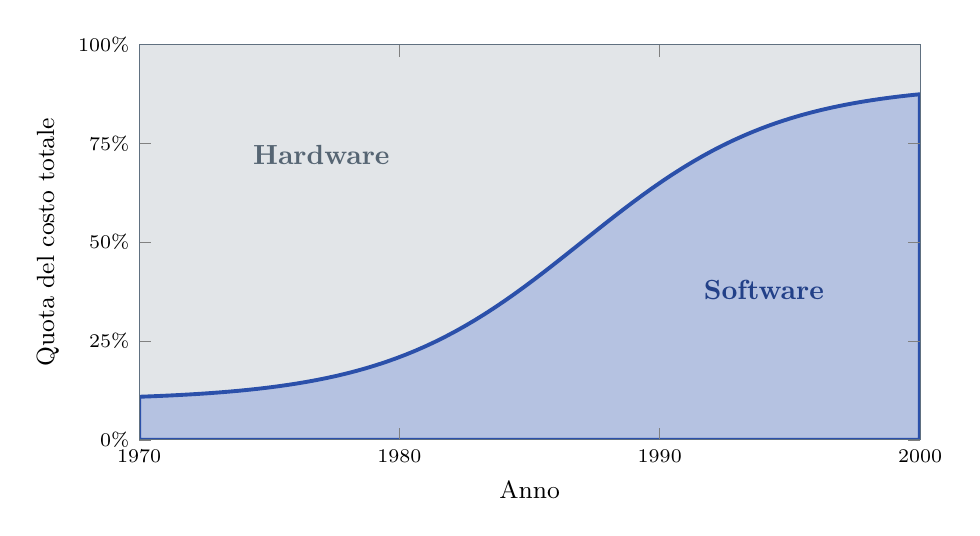
\begin{tikzpicture}
\begin{axis}[
  width=11.5cm, height=6.6cm,
  xmin=1970, xmax=2000, ymin=0, ymax=100,
  xtick={1970,1980,1990,2000},
  x tick label style={/pgf/number format/1000 sep=},
  ytick={0,25,50,75,100},
  yticklabel={\pgfmathprintnumber{\tick}\%},
  xlabel={Anno}, ylabel={Quota del costo totale},
  label style={font=\small}, tick label style={font=\scriptsize},
  axis on top, axis line style={swgray},
]
  \fill[swgray!18] (axis cs:1970,0) rectangle (axis cs:2000,100);
  \addplot[domain=1970:2000, samples=80, fill=swblue!35, draw=swblue, line width=1.4pt]
     {10+80/(1+exp(-(x-1987)/3.8))} \closedcycle;
  \node[font=\bfseries, text=swgray!90!black] at (axis cs:1977,72) {Hardware};
  \node[font=\bfseries, text=swblue!80!black] at (axis cs:1994,38) {Software};
\end{axis}
\end{tikzpicture}
\caption{Andamento qualitativo dei costi relativi di hardware e software (da D. Bell, \textit{Software Engineering for Students}).}
\end{figure}

\subsection{Dove vanno i soldi: i costi per fase}

Ancora più interessante è vedere \textbf{come} si distribuiscono i costi tra le varie fasi della vita di un software.

\begin{figure}[H]
\centering
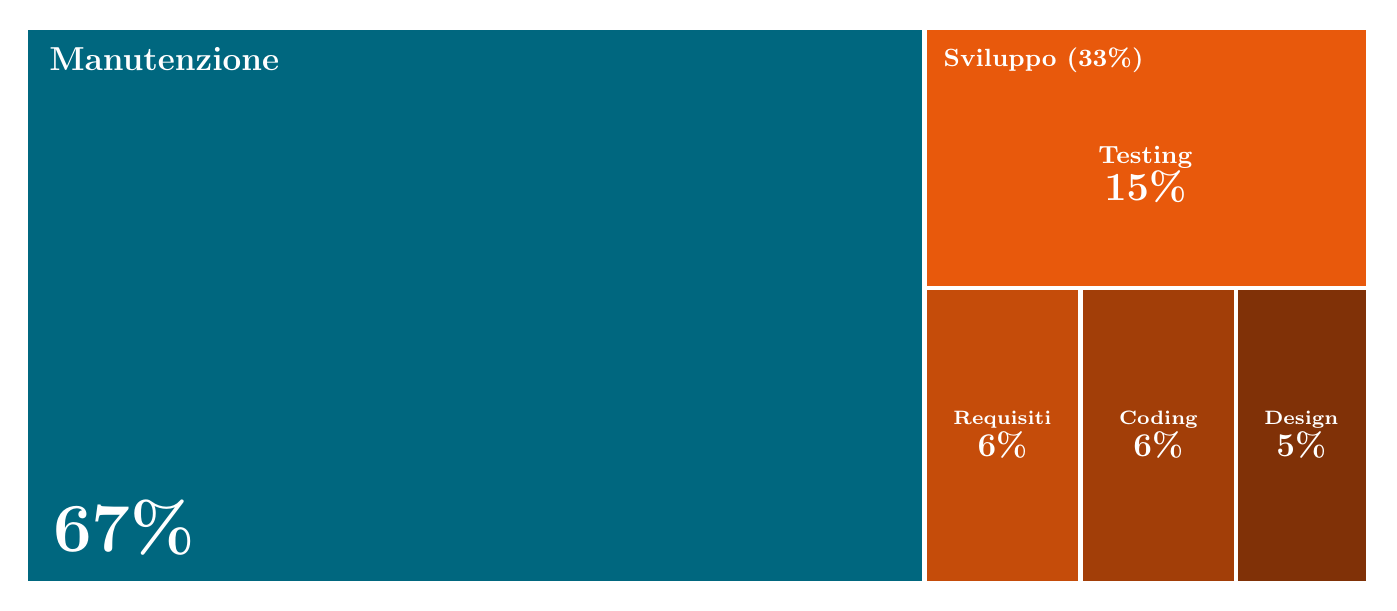
\begin{tikzpicture}
  \def\tmW{17}\def\tmH{7}
  \pgfmathsetmacro{\tmM}{\tmW*0.67}
  \pgfmathsetmacro{\tmD}{\tmW-\tmM}
  \pgfmathsetmacro{\tmT}{\tmH*15/32}
  \pgfmathsetmacro{\tmB}{\tmH-\tmT}
  \pgfmathsetmacro{\tmA}{\tmD*6/17}
  \pgfmathsetmacro{\tmBB}{\tmD*6/17}
  % Manutenzione
  \fill[swteal] (0,0) rectangle (\tmM,\tmH);
  \node[anchor=north west, text=white, font=\large\bfseries] at (0.15,\tmH-0.1) {Manutenzione};
  \node[anchor=south west, text=white, font=\Huge\bfseries] at (0.2,0.2) {67\%};
  % Sviluppo
  \fill[sworange] (\tmM,\tmB) rectangle (\tmW,\tmH);
  \node[anchor=north west, text=white, font=\small\bfseries] at (\tmM+0.12,\tmH-0.1) {Sviluppo (33\%)};
  \node[text=white, font=\small\bfseries, align=center] at (\tmM+\tmD/2,\tmB+\tmT/2-0.2) {Testing\\\Large 15\%};
  \fill[sworange!85!black] (\tmM,0) rectangle (\tmM+\tmA,\tmB);
  \fill[sworange!70!black] (\tmM+\tmA,0) rectangle (\tmM+\tmA+\tmBB,\tmB);
  \fill[sworange!55!black] (\tmM+\tmA+\tmBB,0) rectangle (\tmW,\tmB);
  \node[text=white, font=\scriptsize\bfseries, align=center] at (\tmM+\tmA/2,\tmB/2) {Requisiti\\\large 6\%};
  \node[text=white, font=\scriptsize\bfseries, align=center] at (\tmM+\tmA+\tmBB/2,\tmB/2) {Coding\\\large 6\%};
  \node[text=white, font=\scriptsize\bfseries, align=center] at ({\tmM+\tmA+\tmBB+(\tmW-\tmM-\tmA-\tmBB)/2},\tmB/2) {Design\\\large 5\%};
  \draw[white, line width=1.5pt] (\tmM,0) -- (\tmM,\tmH) (\tmM,\tmB) -- (\tmW,\tmB) (\tmM+\tmA,0) -- (\tmM+\tmA,\tmB) (\tmM+\tmA+\tmBB,0) -- (\tmM+\tmA+\tmBB,\tmB);
\end{tikzpicture}
\caption{Costi relativi delle fasi di un processo software: l'area di ogni rettangolo è proporzionale al costo (da D. Bell).}
\end{figure}

Questo grafico contiene alcune delle lezioni più importanti dell'intero corso:

\begin{enumerate}
  \item \textbf{La manutenzione costa circa il doppio di tutto lo sviluppo messo insieme.} Il grosso della spesa arriva
        \textit{dopo} il rilascio.
  \item \textbf{Scrivere codice è una frazione piccola del totale} (circa il 6\%). Chi pensa che «fare software» significhi
        «programmare» sta guardando solo una piccola parte del problema.
  \item \textbf{Il testing costa più della programmazione}: verificare che il software funzioni è un lavoro enorme.
\end{enumerate}

\info{La conseguenza pratica: progettare per il cambiamento}{
  Se due terzi del costo sono manutenzione, allora conviene investire nelle fasi iniziali (requisiti e progettazione)
  per ottenere un software \textbf{facile da modificare}: modulare, leggibile, ben documentato e ben testato.
  Ogni ora risparmiata «scrivendo codice di fretta» si paga con gli interessi negli anni di manutenzione.
}

\warning{Prendere i numeri con le pinze}{
  Le percentuali esatte variano molto da progetto a progetto e da studio a studio. Quello che conta è l'\textbf{ordine di grandezza}:
  la manutenzione domina, la scrittura del codice è una parte minoritaria.
}

% ============================================================
\section{I modelli di processo}

Un processo software reale è pieno di dettagli: persone, documenti, riunioni, strumenti, eccezioni. Per ragionarci sopra
servono delle rappresentazioni semplificate.

\dfn{Modello di processo software (SDLC)}{
  Un \textbf{Software Process Model}, detto anche \textbf{Software Development Life Cycle (SDLC)}, è una
  \textbf{rappresentazione semplificata} di un processo software. Un modello può concentrarsi su una particolare
  \textbf{prospettiva} (ad esempio la sequenza delle attività, i ruoli coinvolti o i documenti prodotti).
}

Il rapporto tra modello e processo è lo stesso che c'è tra una \textbf{cartina} e il \textbf{territorio}: la cartina
non riporta ogni albero, ma è proprio questa semplificazione a renderla utile. E come esistono cartine diverse per scopi diversi
(stradale, topografica, dei sentieri), esistono modelli di processo diversi che mettono in luce aspetti diversi.

Nel corso vedremo alcuni modelli di processo molto generali:

\begin{figure}[H]
\centering
\begin{tikzpicture}
  % Plan-driven
  \node[chip=swblue, minimum width=7.8cm, minimum height=0.7cm, font=\small\bfseries] (t1) at (0,0) {Modelli guidati dal piano (\textit{plan-driven})};
  \foreach \i/\c in {0/ph1,1/ph2,2/ph3,3/ph4,4/ph5,5/ph6}{
    \fill[\c] (-3.6+\i*1.25,-1.0-\i*0.32) rectangle ++(1.05,-0.42);
  }
  \foreach \i in {0,...,4}{
    \draw[-{Stealth[length=1.5mm]}, swgray] (-2.55+\i*1.25,-1.21-\i*0.32) -| (-2.35+\i*1.25,-1.32-\i*0.32);
  }
  \node[note, text width=7.6cm, align=center, font=\small] at (0,-3.95) {Tutto viene pianificato all'inizio; le fasi si susseguono in ordine.\\\textbf{Esempio}: il modello a cascata (\textit{Waterfall}) --- \textit{prossimo capitolo}.};

  % Incremental / agile
  \node[chip=sworange, minimum width=7.8cm, minimum height=0.7cm, font=\small\bfseries, right=1.2cm of t1] (t2) {Modelli incrementali e agili};
  \foreach \k in {0,1,2}{
    \begin{scope}[shift={(6.3+\k*2.6,-1.75)}]
      \draw[sworange, line width=1.3pt, -{Stealth[length=2mm]}] (0:0.75) arc (0:320:0.75);
      \node[font=\scriptsize\bfseries, text=sworange!80!black] at (0,0) {v\the\numexpr\k+1\relax};
    \end{scope}
  }
  \draw[-{Stealth}, swgray, line width=1pt] (7.1,-1.75) -- (7.8,-1.75);
  \draw[-{Stealth}, swgray, line width=1pt] (9.7,-1.75) -- (10.4,-1.75);
  \node[note, text width=7.6cm, align=center, font=\small] at (8.9,-3.95) {Il software cresce per piccoli incrementi, ripetendo le attività in cicli brevi.\\\textbf{Esempio}: modelli incrementali, metodologie agili --- \textit{più avanti nel corso}.};
\end{tikzpicture}
\caption{Due grandi famiglie di modelli di processo.}
\end{figure}

\gbox{In sintesi}{azure-gradient-6!80!black}{
\begin{itemize}
  \item Un \textbf{processo software} è un insieme di attività correlate che porta alla produzione di software. Non ne esiste uno universale.
  \item Ogni processo comprende \textbf{specifica, implementazione, validazione ed evoluzione}, più attività di supporto come pianificazione e monitoraggio.
  \item Queste attività formano il \textbf{ciclo di vita}: dalla richiesta alla dismissione, con la manutenzione come fase più lunga.
  \item La \textbf{manutenzione} è la voce di costo principale (circa 2/3): bisogna progettare pensando al cambiamento.
  \item Un \textbf{modello di processo (SDLC)} è una rappresentazione semplificata di un processo. Il primo che studiamo è il modello a cascata.
\end{itemize}
}


  \chapter{Il modello a cascata}

\section{Origini e caratteristiche}

Il primo modello di processo che studiamo è anche il più semplice e il più «storico»: il \hi{modello a cascata}
(\textit{Waterfall model}). Deriva dai modelli di processo usati nell'ingegneria dei grandi \textbf{sistemi militari}
ed è stato descritto per il software da Winston W. Royce nel 1970.

Le sue caratteristiche fondamentali sono quattro:

\begin{enumerate}
  \item il processo è composto da una serie di \textbf{fasi sequenziali}: ne finisce una e ne inizia un'altra;
  \item è un processo \textbf{guidato dal piano} (\textit{plan-driven}): tutte le attività vengono pianificate all'inizio e
        l'avanzamento si misura rispetto al piano;
  \item il risultato di ogni fase è un \textbf{documento} che deve essere \textbf{approvato} formalmente (\textit{signed-off});
  \item la fase successiva \textbf{non può iniziare} finché il risultato della fase precedente non è completo.
\end{enumerate}

\begin{figure}[H]
\centering
\begin{tikzpicture}[x=2.9cm, y=1.2cm]
  \foreach \i/\nome/\col in {1/{Requirements\\Engineering}/ph1,
                             2/{System\\Design}/ph2,
                             3/{Software e\\UI Design}/ph3,
                             4/{Implemen-\\tation}/ph4,
                             5/{Testing}/ph5,
                             6/{Operation e\\Maintenance}/ph6}{
    \node[phase=\col, drop shadow] (p\i) at (\i-1,-\i+1) {\nome};
  }
  \foreach \i [evaluate=\i as \j using int(\i+1)] in {1,...,5}{
    \draw[flow] (p\i.east) -| (p\j.north);
  }
  \foreach \j/\doc in {2/{Specifica dei requisiti (SRS)},
                       3/{Architettura del sistema},
                       4/{Specifiche di progetto (UML, mock-up)},
                       5/{Codice sorgente e artefatti},
                       6/{Sistema testato e report dei test}}{
    \node[anchor=east, font=\scriptsize, text width=2.55cm, align=right, text=swgray!80!black] at ([xshift=-0.12cm]p\j.west) {\ifile\ \doc\ {\color{swgreen}\itick}};
  }
\end{tikzpicture}
\caption{Il modello a cascata. A sinistra di ogni fase, il documento (approvato) prodotto dalla fase precedente.}
\end{figure}

\subsection{Perché «a cascata»?}

Il nome deriva dalla forma del diagramma: ogni fase «riversa» il proprio risultato nella successiva, proprio come l'acqua
di una cascata scende da un gradino all'altro. E come l'acqua, il flusso è pensato per andare \textbf{in una sola direzione}: verso il basso.

\warning{Nome e difetto sono due cose diverse}{
  Il nome viene dalla forma del diagramma, non dal fatto che «bisogna tornare indietro». Il ritorno all'indietro
  (che vedremo più avanti) è invece la \textbf{conseguenza} più critica di questa struttura: poiché il modello non prevede
  di risalire la cascata, correggere un errore scoperto tardi costa moltissimo.
}

\info{Curiosità: Royce non era un fan della cascata pura}{
  Nel suo articolo del 1970 Royce presentava il modello sequenziale puro come \textbf{rischioso} e proponeva già dei correttivi:
  tornare alle fasi precedenti, costruire un prototipo prima del sistema definitivo, coinvolgere il cliente durante il processo.
  Ironia della sorte, è passata alla storia soprattutto la versione rigida che lui stesso criticava.
}

% ============================================================
\section{Le sei fasi in sintesi}

Prima di approfondire le singole fasi, ecco una visione d'insieme.

\begin{table}[H]
\centering
\renewcommand{\arraystretch}{1.45}
\begin{tabularx}{\textwidth}{>{\bfseries}P{3.0cm} >{\itshape}P{3.6cm} L P{3.3cm}}
\toprule
Fase & Domanda guida & Cosa si fa & Output principale \\
\midrule
\textcolor{ph1}{Requirements Engineering} & Cosa deve fare il sistema? & Raccolta e specifica dei requisiti insieme a clienti e utenti & Documento di specifica dei requisiti (SRS) \\
\textcolor{ph2}{System Design} & Com'è organizzato il sistema, a grandi linee? & Architettura: moduli, responsabilità, allocazione su hardware & Documento di architettura \\
\textcolor{ph3}{Software e UI Design} & Come si realizza ogni modulo? & Classi, design pattern, prototipi dell'interfaccia & Specifiche di progetto (UML, wireframe) \\
\textcolor{ph4}{Implementation} & Come lo scrivo bene? & Traduzione del progetto in codice «pulito» & Codice sorgente e artefatti \\
\textcolor{ph5}{Testing} & Funziona? È ciò che serviva? & Verifica e validazione: ispezioni e test & Report dei test, sistema pronto \\
\textcolor{ph6}{Operation e Maintenance} & Come lo mantengo in vita? & Installazione, uso reale, correzioni e adattamenti & Nuove versioni del sistema \\
\bottomrule
\end{tabularx}
\caption{Panoramica delle fasi del modello a cascata.}
\end{table}

Le sei fasi non sono altro che un modo più dettagliato di organizzare le \textbf{quattro attività fondamentali}
viste nel capitolo precedente:

\begin{figure}[H]
\centering
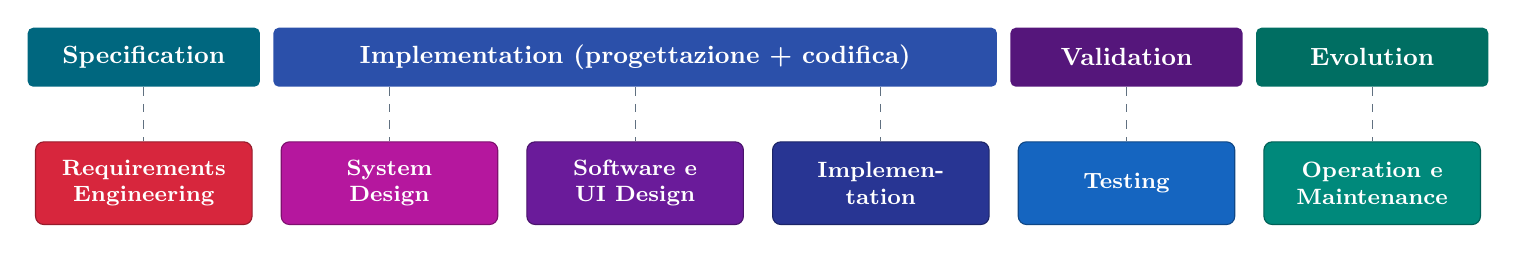
\begin{tikzpicture}[x=3.12cm]
  \foreach \i/\nome/\col in {1/{Requirements\\Engineering}/ph1, 2/{System\\Design}/ph2, 3/{Software e\\UI Design}/ph3,
                             4/{Implemen-\\tation}/ph4, 5/{Testing}/ph5, 6/{Operation e\\Maintenance}/ph6}{
    \node[phase=\col] (m\i) at (\i,0) {\nome};
  }
  \node[chip=swteal, minimum width=2.95cm, minimum height=0.75cm, font=\small\bfseries] (A1) at (1,1.6) {Specification};
  \node[chip=swblue, minimum width=9.19cm, minimum height=0.75cm, font=\small\bfseries] (A2) at (3,1.6) {Implementation (progettazione + codifica)};
  \node[chip=ph3!80!black, minimum width=2.95cm, minimum height=0.75cm, font=\small\bfseries] (A3) at (5,1.6) {Validation};
  \node[chip=ph6!80!black, minimum width=2.95cm, minimum height=0.75cm, font=\small\bfseries] (A4) at (6,1.6) {Evolution};
  \foreach \i/\a in {1/A1,2/A2,3/A2,4/A2,5/A3,6/A4}{
    \draw[swgray, dashed] (\a.south -| m\i.north) -- (m\i.north);
  }
\end{tikzpicture}
\caption{Corrispondenza tra le quattro attività fondamentali e le sei fasi del modello a cascata.}
\end{figure}

% ============================================================
\section{Fase 1: Requirements Engineering}

\waterfallbar{1}

\dfn{Ingegneria dei requisiti}{
  Fase in cui si cerca di capire \textbf{cosa} il software da realizzare (\textit{software-to-be}) deve fare,
  \textbf{non come} implementarlo. Richiede un'analisi attenta dei bisogni degli utenti e del dominio del problema e coinvolge
  clienti, utenti finali e ingegneri del software. L'output principale è il \textbf{documento di specifica dei requisiti}
  (\textit{Software Requirements Specification}, SRS).
}

È una fase di \textbf{modellazione}: non si costruisce ancora la soluzione, ma un \textbf{modello di ciò che il sistema dovrà fare},
sia in termini di \textbf{funzionalità} sia in termini di \textbf{qualità}. Per questo:
\begin{itemize}
  \item \textbf{non si scrive codice}: si producono documenti e diagrammi;
  \item \textbf{non si fanno scelte tecnologiche} (linguaggi, database, framework) e non si parla di hardware, a meno che non si tratti
        di un \textbf{vincolo} imposto dal cliente (ad esempio: «il sistema deve girare sui server già presenti in azienda»);
  \item si guarda il sistema \textbf{dall'esterno}, come una scatola nera: cosa vede e cosa fa l'utente, come interagisce con il sistema,
        non come il sistema è fatto dentro.
\end{itemize}

Questa fase è così importante da meritare un capitolo a parte: la riprenderemo in dettaglio nel Capitolo 5.

\subsection{Cosa, non come}

La distinzione tra \textit{cosa} e \textit{come} è la più importante di questa fase. Vediamola su un sistema per una biblioteca:

\begin{table}[H]
\centering
\renewcommand{\arraystretch}{1.4}
\begin{tabularx}{\textwidth}{L >{\centering\arraybackslash}p{3.4cm}}
\toprule
Affermazione & È un requisito? \\
\midrule
L'utente deve poter cercare un libro per titolo, autore o ISBN. & {\color{swgreen}\itick} Sì (cosa) \\
Il risultato della ricerca deve comparire entro 2 secondi. & {\color{swgreen}\itick} Sì (qualità) \\
La ricerca usa un indice sulla tabella \texttt{LIBRI} di un database MySQL. & {\color{swred}\icross} No (come) \\
La classe \texttt{RicercaService} espone il metodo \texttt{cerca(String)}. & {\color{swred}\icross} No (come) \\
Il sistema deve funzionare sui computer Windows già presenti in biblioteca. & {\color{swgreen}\itick} Sì (vincolo) \\
\bottomrule
\end{tabularx}
\caption{Requisiti (cosa) e decisioni di progetto (come).}
\end{table}

\subsection{Requisiti funzionali e non funzionali}

Il modello del sistema descrive sia le funzionalità sia le qualità. Da qui la distinzione classica:

\begin{center}
\begin{tikzpicture}
  \node[card=ph1, text width=7.8cm, align=left, minimum height=3.3cm] (f) {%
    \textbf{Requisiti funzionali}\\[3pt]
    \small Descrivono \textbf{cosa} il sistema deve fare: servizi offerti, reazioni agli input, comportamento in situazioni specifiche.\\[4pt]
    \scriptsize\textit{Es.}: «Il bibliotecario può registrare la restituzione di un libro.»\\
    \scriptsize\textit{Es.}: «L'utente riceve un'e-mail tre giorni prima della scadenza del prestito.»};
  \node[card=ph3, text width=7.8cm, align=left, minimum height=3.3cm, right=0.5cm of f] (nf) {%
    \textbf{Requisiti non funzionali (di qualità)}\\[3pt]
    \small Descrivono \textbf{quanto bene} il sistema deve farlo e con quali vincoli: prestazioni, sicurezza, usabilità, affidabilità\ldots\\[4pt]
    \scriptsize\textit{Es.}: «Il catalogo deve essere disponibile 24 ore su 24.»\\
    \scriptsize\textit{Es.}: «Solo il personale autenticato può modificare i prestiti.»};
\end{tikzpicture}
\end{center}

I requisiti non funzionali si collegano direttamente ai \textbf{modelli di qualità} che studieremo nel Capitolo 4.

\subsection{Tecniche per raccogliere e specificare i requisiti}

\begin{table}[H]
\centering
\renewcommand{\arraystretch}{1.4}
\begin{tabularx}{\textwidth}{>{\bfseries}P{3.4cm} L}
\toprule
\multicolumn{2}{l}{\textcolor{ph1}{\textbf{Raccolta} (\textit{elicitation})}} \\
\midrule
Interviste & Colloqui con gli \textit{stakeholder} (clienti, utenti, esperti del dominio) per capire bisogni e problemi. \\
Personas & Utenti «tipo» immaginari ma realistici (es.\ «Anna, 68 anni, poco pratica di tecnologia») usati per non perdere di vista chi userà davvero il sistema. \\
Storie e scenari & Racconti concreti di come un utente usa il sistema per raggiungere un obiettivo. \\
\midrule
\multicolumn{2}{l}{\textcolor{ph1}{\textbf{Specifica}}} \\
\midrule
Casi d'uso & Descrivono le interazioni tra gli attori (utenti o altri sistemi) e il sistema per raggiungere un obiettivo. \\
Linguaggio naturale & Requisiti scritti in frasi, possibilmente brevi, precise e verificabili. \\
Modelli di dominio & Diagrammi dei concetti del mondo reale e delle loro relazioni (es.\ Libro, Prestito, Utente). \\
Mock-up & Bozze dell'interfaccia che aiutano cliente e sviluppatori a capirsi. \\
\bottomrule
\end{tabularx}
\end{table}

\dfn{Stakeholder}{
  Qualsiasi persona o organizzazione che ha un \textbf{interesse} nel sistema o ne è \textbf{influenzata}: il cliente che paga,
  gli utenti finali, il personale che lo manterrà, ma anche, ad esempio, un ente regolatore.
}

\begin{esempio}{Un diagramma dei casi d'uso per la biblioteca}
\begin{center}
\begin{tikzpicture}
  \draw[rounded corners=4pt, line width=0.9pt, swgray] (-3.3,-2.4) rectangle (3.3,2.4);
  \node[font=\small\bfseries, text=swgray, anchor=north] at (0,2.35) {Sistema Biblioteca};
  \stickman{(-5.4,0.2)}{Utente}
  \stickman{(5.4,0.2)}{Bibliotecario}
  \node[ellipse, draw=ph1, fill=ph1!8, line width=0.8pt, minimum width=3.6cm, minimum height=0.8cm, font=\scriptsize] (u1) at (0,1.35) {Cerca libro};
  \node[ellipse, draw=ph1, fill=ph1!8, line width=0.8pt, minimum width=3.6cm, minimum height=0.8cm, font=\scriptsize] (u2) at (0,0.2) {Prenota libro};
  \node[ellipse, draw=ph1, fill=ph1!8, line width=0.8pt, minimum width=3.6cm, minimum height=0.8cm, font=\scriptsize] (u3) at (0,-0.95) {Registra prestito};
  \node[ellipse, draw=ph1, fill=ph1!8, line width=0.8pt, minimum width=3.6cm, minimum height=0.8cm, font=\scriptsize] (u4) at (0,-1.95) {Registra restituzione};
  \draw (-5.1,0.45) -- (u1.west);
  \draw (-5.1,0.45) -- (u2.west);
  \draw (5.1,0.45) -- (u1.east);
  \draw (5.1,0.45) -- (u3.east);
  \draw (5.1,0.45) -- (u4.east);
\end{tikzpicture}
\end{center}
Gli \textbf{attori} (omini) sono all'esterno del sistema; i \textbf{casi d'uso} (ellissi) sono gli obiettivi che gli attori
raggiungono usando il sistema. Il diagramma dice \textit{cosa} si può fare, senza dire nulla su \textit{come} sarà realizzato.
\end{esempio}

\warning{Il cliente non sa sempre cosa vuole}{
  I requisiti raccolti possono essere \textbf{incompleti}, \textbf{ambigui} o persino \textbf{contraddittori} (stakeholder diversi
  vogliono cose diverse). Non a caso, nel progetto d'esame i docenti si comportano come clienti tipici e possono fornire requisiti
  incoerenti: individuarli e chiarirli fa parte del lavoro.
}

% ============================================================
\section{Fase 2: System Design}

\waterfallbar{2}

Una volta chiaro \textit{cosa} fare, si passa al \textit{come}. L'obiettivo delle due fasi di progettazione è definire una
\textbf{struttura adeguata} (architettura) per il software. Si lavora su \textbf{due livelli}: prima quello di sistema (alto livello),
poi quello del singolo modulo (basso livello).

\dfn{System Design (progettazione di sistema)}{
  Definisce l'\textbf{architettura complessiva} del sistema, cioè la sua vista «di massima»:
  \begin{itemize}
    \item la \textbf{decomposizione} in moduli e componenti (sottosistemi);
    \item l'\textbf{allocazione} dei requisiti/funzionalità ai moduli e dei moduli alle risorse hardware;
    \item le \textbf{relazioni e collaborazioni} tra i moduli.
  \end{itemize}
}

Un'analogia: è come la \textbf{pianta di una casa} disegnata dall'architetto. Stabilisce quante stanze ci sono, a cosa servono e come
sono collegate, ma non sceglie ancora il modello delle maniglie.

In questa fase si ricorre spesso a \textbf{pattern architetturali}, cioè soluzioni collaudate per organizzare un sistema:
ad esempio \textit{client-server}, architettura \textit{a livelli} (presentazione, logica, dati) o \textit{Model-View-Controller}.

\begin{esempio}{Architettura di massima di un e-commerce}
\begin{center}
\begin{tikzpicture}[font=\scriptsize]
  % Nodi hardware
  \node[draw=swgray, fill=swlight, rounded corners=3pt, minimum width=3.6cm, minimum height=3.3cm, anchor=north] (hw1) at (0,0) {};
  \node[font=\scriptsize\bfseries, text=swgray, anchor=north] at (hw1.north) {\iwindow\ Dispositivo utente};
  \node[phase=ph2, minimum width=2.9cm, minimum height=0.7cm, font=\scriptsize\bfseries] (ui) at (0,-1.1) {Interfaccia web};
  \node[phase=ph2, fill=ph2!75, minimum width=2.9cm, minimum height=0.7cm, font=\scriptsize\bfseries] (app) at (0,-2.2) {App mobile};

  \node[draw=swgray, fill=swlight, rounded corners=3pt, minimum width=7.6cm, minimum height=3.3cm, anchor=north] (hw2) at (6.4,0) {};
  \node[font=\scriptsize\bfseries, text=swgray, anchor=north] at (hw2.north) {\icpu\ Application server};
  \node[phase=ph2, minimum width=2.1cm, minimum height=0.7cm, font=\scriptsize\bfseries] (m1) at (4.6,-1.1) {Catalogo};
  \node[phase=ph2, minimum width=2.1cm, minimum height=0.7cm, font=\scriptsize\bfseries] (m2) at (6.9,-1.1) {Carrello};
  \node[phase=ph2, minimum width=2.1cm, minimum height=0.7cm, font=\scriptsize\bfseries] (m3) at (4.6,-2.2) {Ordini};
  \node[phase=ph2, minimum width=2.1cm, minimum height=0.7cm, font=\scriptsize\bfseries] (m4) at (6.9,-2.2) {Utenti};
  \node[phase=sworange, minimum width=1.5cm, minimum height=1.8cm, font=\scriptsize\bfseries] (m5) at (9.2,-1.65) {Pagamenti};

  \node[draw=swgray, fill=swlight, rounded corners=3pt, minimum width=3.2cm, minimum height=3.3cm, anchor=north] (hw3) at (12.6,0) {};
  \node[font=\scriptsize\bfseries, text=swgray, anchor=north] at (hw3.north) {\icpu\ Database server};
  \node[cylinder, shape border rotate=90, aspect=0.25, draw=ph2!70!black, fill=ph2!15, minimum width=1.8cm, minimum height=1.5cm, font=\scriptsize\bfseries] (db) at (12.6,-1.8) {Dati};

  \node[draw=swgray, dashed, rounded corners=3pt, minimum width=2.6cm, minimum height=1cm, align=center] (ext) at (9.2,-4.3) {Servizio esterno\\di pagamento};

  \draw[{Stealth}-{Stealth}, line width=0.9pt] (hw1.east |- 0,-1.65) -- node[above]{HTTPS} (hw2.west |- 0,-1.65);
  \draw[{Stealth}-{Stealth}, line width=0.9pt] (hw2.east |- 0,-1.65) -- (hw3.west |- 0,-1.65);
  \draw[{Stealth}-{Stealth}, line width=0.9pt, dashed] (m5.south) -- (ext.north);
\end{tikzpicture}
\end{center}
Il sistema è scomposto in \textbf{moduli} con responsabilità precise (catalogo, carrello, ordini, utenti, pagamenti), i moduli
sono \textbf{allocati} a nodi hardware diversi e sono definite le \textbf{collaborazioni} (chi comunica con chi).
\end{esempio}

\info{Perché progettare in modo modulare}{
  Un sistema ben scomposto in moduli indipendenti è molto più \textbf{flessibile}: se domani cambia il fornitore dei pagamenti,
  si interviene solo sul modulo \textit{Pagamenti} senza toccare il resto. Ricordando che la manutenzione vale circa due terzi
  dei costi, la modularità decisa in questa fase è un investimento che ripaga per anni.
}

% ============================================================
\section{Fase 3: Software e UI Design}

\waterfallbar{3}

\dfn{Software e UI Design (progettazione di dettaglio)}{
  Scende nel \textbf{dettaglio di come implementare ciascun modulo}. Comprende la progettazione dell'architettura software
  di basso livello (quali \textbf{classi e oggetti} servono per realizzare ogni sottosistema?) e la \textbf{prototipazione
  dell'interfaccia utente}.
}

Le principali attività e tecniche sono:
\begin{itemize}
  \item definire gli \textbf{oggetti} (classi, attributi, metodi, relazioni) necessari a realizzare ogni sottosistema;
  \item applicare i \textbf{design pattern}, cioè soluzioni riusabili a problemi di progettazione ricorrenti;
  \item applicare l'\textbf{ingegneria dell'usabilità} per progettare interfacce facili da usare;
  \item produrre \textbf{wireframe ad alta fedeltà}, cioè prototipi dell'interfaccia molto vicini al risultato finale.
\end{itemize}

L'output è un insieme di \textbf{specifiche di progetto}, spesso formalizzate con linguaggi di modellazione come \textbf{UML}.

\begin{figure}[H]
\centering
\begin{minipage}[c]{0.56\textwidth}
\centering
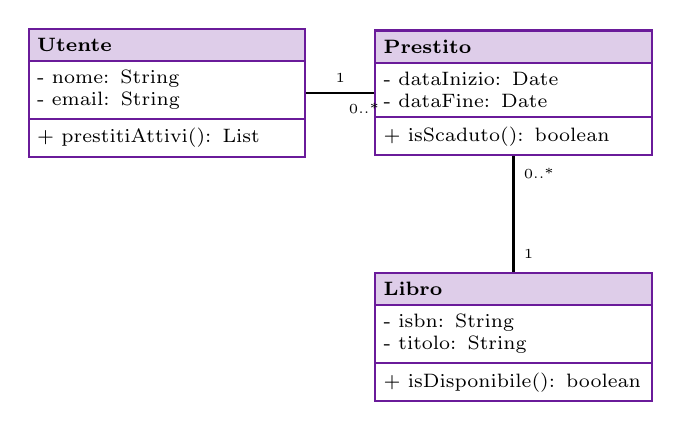
\begin{tikzpicture}[
  cls/.style={rectangle split, rectangle split parts=3, draw=ph3, line width=0.8pt,
              rectangle split part fill={ph3!22,white,white}, font=\scriptsize, align=left,
              text width=3.3cm, inner sep=3pt}]
  \node[cls] (utente) at (0,0) {\centering\textbf{Utente}\nodepart{second}- nome: String\\- email: String\nodepart{third}+ prestitiAttivi(): List};
  \node[cls] (prestito) at (4.4,0) {\centering\textbf{Prestito}\nodepart{second}- dataInizio: Date\\- dataFine: Date\nodepart{third}+ isScaduto(): boolean};
  \node[cls] (libro) at (4.4,-3.1) {\centering\textbf{Libro}\nodepart{second}- isbn: String\\- titolo: String\nodepart{third}+ isDisponibile(): boolean};
  \draw[line width=0.8pt] (utente.east) -- node[above, font=\tiny]{1} node[below, font=\tiny, pos=0.85]{0..*} (prestito.west);
  \draw[line width=0.8pt] (prestito.south) -- node[right, font=\tiny, pos=0.15]{0..*} node[right, font=\tiny, pos=0.85]{1} (libro.north);
\end{tikzpicture}\\[3pt]
{\small (a) Diagramma delle classi UML}
\end{minipage}\hfill
\begin{minipage}[c]{0.40\textwidth}
\centering
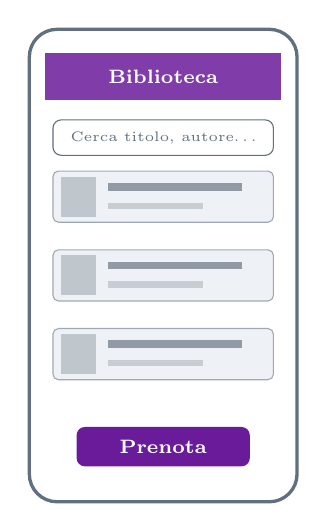
\begin{tikzpicture}
  \draw[rounded corners=10pt, line width=1.2pt, swgray, fill=white] (0,0) rectangle (3.4,6);
  \fill[ph3!85] (0.2,5.1) rectangle (3.2,5.7);
  \node[text=white, font=\scriptsize\bfseries] at (1.7,5.4) {Biblioteca};
  \draw[rounded corners=3pt, swgray] (0.3,4.4) rectangle (3.1,4.85);
  \node[font=\tiny, text=swgray, anchor=west] at (0.4,4.62) {Cerca titolo, autore\ldots};
  \foreach \k in {0,1,2}{
    \draw[rounded corners=2pt, swgray!60, fill=swlight] (0.3,3.55-\k*1.0) rectangle (3.1,4.2-\k*1.0);
    \fill[swgray!40] (0.4,3.62-\k*1.0) rectangle (0.85,4.13-\k*1.0);
    \fill[swgray!70] (1.0,3.95-\k*1.0) rectangle (2.7,4.05-\k*1.0);
    \fill[swgray!35] (1.0,3.72-\k*1.0) rectangle (2.2,3.8-\k*1.0);
  }
  \fill[rounded corners=3pt, ph3] (0.6,0.45) rectangle (2.8,0.95);
  \node[text=white, font=\scriptsize\bfseries] at (1.7,0.7) {Prenota};
\end{tikzpicture}\\[3pt]
{\small (b) Wireframe di una schermata}
\end{minipage}
\caption{Due tipici prodotti della progettazione di dettaglio.}
\end{figure}

\subsection{Alto livello e basso livello a confronto}

\begin{table}[H]
\centering
\renewcommand{\arraystretch}{1.4}
\begin{tabularx}{\textwidth}{>{\bfseries}P{3.2cm} L L}
\toprule
 & \textcolor{ph2}{System Design} & \textcolor{ph3}{Software e UI Design} \\
\midrule
Livello & Alto: il sistema nel suo insieme & Basso: il singolo modulo \\
Elementi & Sottosistemi, componenti, nodi hardware & Classi, oggetti, metodi, schermate \\
Strumenti & Pattern architetturali & Design pattern, usabilità, wireframe \\
Analogia & La pianta della casa & Il progetto esecutivo di ogni stanza (impianti, arredi) \\
Domanda & Quali pezzi e come comunicano? & Come è fatto dentro ogni pezzo? \\
\bottomrule
\end{tabularx}
\end{table}

\warning{Scelte tecnologiche e design pattern: due precisazioni}{
  \begin{itemize}
    \item \textbf{Il linguaggio}: le scelte tecnologiche (linguaggio, framework, database) si concretizzano durante la progettazione,
          quando servono a definire la soluzione, a meno che non siano già un vincolo imposto nei requisiti. Il criterio non è solo
          «il linguaggio migliore in assoluto»: contano l'adeguatezza al problema, le librerie disponibili e le \textbf{competenze del team}.
    \item \textbf{I design pattern} sono in larga parte \textbf{indipendenti dal linguaggio}: descrivono un'idea di soluzione
          (ad esempio «notifica automaticamente gli interessati quando un oggetto cambia stato»). È la loro \textit{implementazione}
          che dipende dalle caratteristiche del linguaggio scelto.
  \end{itemize}
}

% ============================================================
\section{Fase 4: Implementation}

\waterfallbar{4}

\dfn{Implementazione}{
  Fase in cui la specifica di progetto viene \textbf{tradotta} nel linguaggio di programmazione e nelle tecnologie scelte.
  Ogni sottosistema viene implementato, producendo il codice sorgente e gli altri artefatti necessari.
}

Non una traduzione qualsiasi, però: deve essere una traduzione di \textbf{alta qualità}. Il codice risultante deve essere:

\begin{table}[H]
\centering
\renewcommand{\arraystretch}{1.4}
\begin{tabularx}{\textwidth}{>{\bfseries\leavevmode\color{ph4}}P{4.4cm} L}
\toprule
Leggibile (\textit{readable}) & Un altro sviluppatore (o noi tra sei mesi) lo capisce senza fatica? \\
Manutenibile (\textit{maintainable}) & È facile correggerlo o modificarlo senza rompere altro? \\
Riusabile (\textit{reusable}) & Parti del codice possono essere usate in altri contesti? \\
Estendibile (\textit{extendable}) & Si possono aggiungere funzionalità senza stravolgere l'esistente? \\
Testabile (\textit{testable}) & È facile scrivere test automatici che ne verifichino il comportamento? \\
\bottomrule
\end{tabularx}
\end{table}

\ldots o, in una sola parola, \hi{clean} (pulito). Oltre al codice, in questa fase si usano \textbf{framework} (strutture già pronte
che forniscono le fondamenta dell'applicazione) e \textbf{ORM} (\textit{Object-Relational Mapping}: librerie che traducono
automaticamente gli oggetti del programma in righe delle tabelle di un database relazionale e viceversa).

\begin{esempio}{Stesso comportamento, qualità molto diversa}
Entrambe le versioni calcolano il totale di un carrello applicando gli sconti. La prima «funziona», ma è illeggibile:
\Needspace{14\baselineskip}\begin{lstlisting}[language=Java]
public double c(List<double[]> l) {
    double t = 0;
    for (double[] x : l) t += x[0] * x[1] * (1 - x[2]);
    return t;
}
\end{lstlisting}
Cosa sono \texttt{x[0]}, \texttt{x[1]} e \texttt{x[2]}? Senza leggere il resto del programma è impossibile saperlo.
La seconda versione dice esattamente cosa fa:
\Needspace{14\baselineskip}\begin{lstlisting}[language=Java]
public double calcolaTotaleCarrello(List<RigaCarrello> righe) {
    double totale = 0;
    for (RigaCarrello riga : righe) {
        totale += riga.getPrezzoUnitario()
                * riga.getQuantita()
                * (1 - riga.getSconto());
    }
    return totale;
}
\end{lstlisting}
Nomi espressivi e tipi dedicati rendono il codice leggibile, più facile da modificare (es.\ aggiungere l'IVA) e da testare.
\end{esempio}

% ============================================================
\section{Fase 5: Testing}

\waterfallbar{5}

Abbiamo un'implementazione. Ma questa implementazione \textbf{soddisfa davvero i bisogni degli utenti}?
Per rispondere si svolgono le attività di \hi{verifica e validazione} (V\&V). Sono due concetti diversi e spesso confusi.

\dfn{Verifica (Verification)}{
  Il sistema è \textbf{conforme alla sua specifica}? In altre parole: \textit{abbiamo costruito il prodotto nel modo giusto?}
  Si fa tipicamente con il \textbf{testing del programma}: si esegue il software in un ambiente controllato e si controlla che
  il suo comportamento sia corretto rispetto alle specifiche.
}

\dfn{Validazione (Validation)}{
  Il sistema \textbf{soddisfa le aspettative del cliente}? In altre parole: \textit{abbiamo costruito il prodotto giusto?}
  Si fa tipicamente definendo ed eseguendo \textbf{test di accettazione}, spesso insieme al cliente.
}

\begin{figure}[H]
\centering
\begin{tikzpicture}
  \node[card=swteal, minimum width=3.9cm, minimum height=1.3cm] (need) at (0,0) {\iuser\ \textbf{Esigenze reali}\\\scriptsize del cliente};
  \node[card=ph1, minimum width=3.9cm, minimum height=1.3cm] (spec) at (6.2,0) {\ifile\ \textbf{Specifica}\\\scriptsize (requisiti scritti)};
  \node[card=ph4, minimum width=3.9cm, minimum height=1.3cm] (sys) at (12.4,0) {\icpu\ \textbf{Sistema}\\\scriptsize realizzato};
  \draw[flow] (need) -- node[above, font=\scriptsize]{analisi} (spec);
  \draw[flow] (spec) -- node[above, font=\scriptsize]{sviluppo} (sys);
  \draw[{Stealth[length=2.6mm]}-{Stealth[length=2.6mm]}, line width=1.3pt, ph5] (sys.south) to[out=-120, in=-60] node[below, font=\small\bfseries, text=ph5, align=center]{VERIFICA\\\scriptsize\normalfont «nel modo giusto?»} (spec.south);
  \draw[{Stealth[length=2.6mm]}-{Stealth[length=2.6mm]}, line width=1.3pt, swred] (sys.north) to[out=140, in=40] node[above, font=\small\bfseries, text=swred, align=center]{\scriptsize\normalfont «il prodotto giusto?»\\VALIDAZIONE} (need.north);
\end{tikzpicture}
\caption{La verifica confronta il sistema con la specifica; la validazione lo confronta con le esigenze reali.}
\end{figure}

\begin{esempio}{Verificato ma non validato}
La specifica dice: «il sistema deve esportare il report mensile delle vendite in PDF». Gli sviluppatori realizzano un'esportazione
PDF perfetta: tutti i test passano, quindi il sistema è \textbf{verificato}. Alla consegna, però, il cliente scopre che il suo
ufficio contabilità ha bisogno di \textit{rielaborare} quei dati in un foglio di calcolo: un PDF non gli serve a nulla.
Il sistema \textbf{non è validato}. L'errore non è nel codice, ma nei requisiti.
\end{esempio}

\subsection{Le attività di testing}

\begin{itemize}
  \item \textbf{Ispezioni del codice} (\textit{code inspection}): il codice viene letto ed esaminato da altre persone \textit{senza eseguirlo},
        alla ricerca di errori e cattive pratiche.
  \item \textbf{Test funzionale}: si esegue il software e si confrontano i risultati con quelli attesi. Si svolge a più livelli:
        \textit{unità}, \textit{integrazione}, \textit{sistema}.
  \item \textbf{Test di usabilità}: si osservano utenti reali mentre usano il sistema per scoprire difficoltà dell'interfaccia.
\end{itemize}

I livelli del test funzionale procedono dal piccolo al grande: si controlla che \textbf{metodo per metodo} e \textbf{classe per classe}
il codice faccia quello che deve, poi che i \textbf{moduli} funzionino insieme e infine che l'\textbf{intero sistema} rispetti i requisiti.

\begin{figure}[H]
\centering
\begin{tikzpicture}
  \draw[rounded corners=6pt, fill=ph5!8, draw=ph5, line width=1pt] (0,0) rectangle (10.4,5.4);
  \node[anchor=north west, font=\small\bfseries, text=ph5] at (0.15,5.35) {Sistema};
  \foreach \m/\x in {A/0.4, B/5.4}{
    \draw[rounded corners=5pt, fill=ph5!15, draw=ph5!80, line width=0.8pt] (\x,0.35) rectangle (\x+4.6,4.6);
    \node[anchor=north west, font=\scriptsize\bfseries, text=ph5!90!black] at (\x+0.1,4.55) {Modulo \m};
    \foreach \c/\cx in {1/0.25, 2/2.4}{
      \draw[rounded corners=3pt, fill=white, draw=ph4!70, line width=0.7pt] (\x+\cx,0.7) rectangle (\x+\cx+1.95,3.8);
      \node[anchor=north west, font=\tiny\bfseries, text=ph4] at (\x+\cx+0.05,3.75) {Classe \m\c};
      \foreach \k in {0,1,2}{
        \draw[rounded corners=2pt, fill=ph4!12, draw=ph4!50] (\x+\cx+0.2,2.75-\k*0.65) rectangle (\x+\cx+1.75,3.2-\k*0.65);
        \node[font=\tiny, text=ph4!80!black] at (\x+\cx+0.975,2.975-\k*0.65) {metodo()};
      }
    }
  }
  \draw[{Stealth}-{Stealth}, line width=0.9pt, sworange] (5.0,2.3) -- (5.4,2.3);
  \node[card=ph4, anchor=west, text width=5.3cm, align=left, font=\scriptsize] at (11,4.4) {\textbf{Test di unità}: un metodo o una classe, isolati dal resto.};
  \node[card=sworange, anchor=west, text width=5.3cm, align=left, font=\scriptsize] at (11,2.7) {\textbf{Test di integrazione}: più moduli (o classi) che collaborano.};
  \node[card=ph5, anchor=west, text width=5.3cm, align=left, font=\scriptsize] at (11,1.0) {\textbf{Test di sistema}: l'intero sistema, confrontato con i requisiti.};
\end{tikzpicture}
\caption{I livelli del test funzionale, dal più piccolo al più grande.}
\end{figure}

\info{Per approfondire: il modello a V}{
  Una variante molto diffusa del modello a cascata, il \textbf{modello a V}, rende esplicito che ogni fase di progettazione
  ha una fase di test «gemella» che ne verifica il risultato:
  \begin{center}
  \begin{tikzpicture}[font=\scriptsize\bfseries]
    \node[phase=ph1, minimum width=2.6cm, minimum height=0.7cm] (r) at (0,0) {Requisiti};
    \node[phase=ph2, minimum width=2.6cm, minimum height=0.7cm] (s) at (1.3,-1.0) {System Design};
    \node[phase=ph3, minimum width=2.6cm, minimum height=0.7cm] (d) at (2.6,-2.0) {Software Design};
    \node[phase=ph4, minimum width=2.6cm, minimum height=0.7cm] (i) at (5.2,-3.0) {Implementazione};
    \node[phase=ph5, minimum width=2.6cm, minimum height=0.7cm] (tu) at (7.8,-2.0) {Test di integrazione};
    \node[phase=ph5, minimum width=2.6cm, minimum height=0.7cm] (ts) at (9.1,-1.0) {Test di sistema};
    \node[phase=ph5, minimum width=2.6cm, minimum height=0.7cm] (ta) at (10.4,0) {Test di accettazione};
    \draw[flow] (r) -- (s); \draw[flow] (s) -- (d); \draw[flow] (d) |- (i); \draw[flow] (i) -| (tu); \draw[flow] (tu) -- (ts); \draw[flow] (ts) -- (ta);
    \draw[swred, dashed, {Stealth}-{Stealth}] (r) -- node[above, font=\tiny\normalfont, text=swred]{validazione} (ta);
    \draw[ph5, dashed, {Stealth}-{Stealth}] (s) -- (ts);
    \draw[ph5, dashed, {Stealth}-{Stealth}] (d) -- (tu);
    \node[font=\tiny\normalfont, text=ph4, below=0.05cm of i] {+ test di unità};
  \end{tikzpicture}
  \end{center}
  Il testing verrà ripreso durante il corso ed è l'argomento centrale del corso magistrale di \textit{Software Testing}.
}

% ============================================================
\section{Fase 6: Operation e Maintenance}

\waterfallbar{6}

\dfn{Esercizio (Operation)}{
  Il sistema viene \textbf{distribuito e installato} presso i clienti e messo in \textbf{uso reale}.
}

\dfn{Manutenzione (Maintenance)}{
  Prima o poi il software \textbf{dovrà cambiare}. La manutenzione comprende tutte le modifiche apportate dopo il rilascio.
}

I motivi per cui il software cambia sono essenzialmente tre:
\begin{itemize}
  \item cambiano le \textbf{esigenze del cliente} (nuove funzionalità, processi aziendali diversi);
  \item cambia il \textbf{contesto d'uso} (ad esempio entra in vigore una nuova legge che richiede procedure diverse,
        oppure esce un nuovo sistema operativo);
  \item emergono \textbf{bug} sfuggiti alla fase di verifica e validazione.
\end{itemize}

Questi motivi corrispondono alla classificazione tradizionale dei tipi di manutenzione:

\begin{table}[H]
\centering
\renewcommand{\arraystretch}{1.45}
\begin{tabularx}{\textwidth}{>{\bfseries}P{2.6cm} L L}
\toprule
Tipo & Scopo & Esempio \\
\midrule
\textcolor{swred}{Correttiva} & Correggere errori non scoperti nelle fasi precedenti & Il calcolo degli interessi sbaglia l'arrotondamento negli anni bisestili \\
\textcolor{sworange}{Adattiva} & Adattare il software a un ambiente che cambia & Aggiornare l'app per la nuova versione di Android; recepire una nuova normativa fiscale \\
\textcolor{swblue}{Perfettiva} & Migliorare o aggiungere funzionalità su richiesta & Il cliente chiede di poter pagare anche con lo smartphone \\
\textcolor{swgreen}{Preventiva} & Rendere il software più facile da mantenere in futuro & Ristrutturare (\textit{refactoring}) un modulo diventato troppo complicato \\
\bottomrule
\end{tabularx}
\caption{I tipi di manutenzione.}
\end{table}

\info{Un problema specifico della cascata}{
  Nel modello a cascata la manutenzione è l'ultima fase, ma una modifica importante (ad esempio un nuovo requisito) non si può
  «fare e basta»: richiede di \textbf{ripercorrere le fasi} a partire da quella interessata, aggiornando e riapprovando requisiti,
  progetto, codice e test. È qui che la rigidità del modello si fa sentire di più.
  L'evoluzione del software è approfondita nel corso magistrale di \textit{Software Project Management and Evolution}.
}

% ============================================================
\section{Il problema del ritorno all'indietro}

Un approccio rigido e «a senso unico» (\textit{feed-forward}) ha senso nell'\textbf{ingegneria dell'hardware}, dove i costi di produzione sono
altissimi: una volta prodotti migliaia di chip, o costruito un ponte, non si torna indietro. Per questo è essenziale aver completato
e approvato ogni fase prima di passare alla successiva.

Nello sviluppo software, invece, le fasi \textbf{si sovrappongono e si scambiano informazioni} di continuo:
\begin{itemize}
  \item durante il \textbf{System Design} si scoprono problemi nei \textbf{requisiti} (ambigui, incompleti, impossibili da realizzare);
  \item durante l'\textbf{implementazione} si scoprono problemi nel \textbf{progetto};
  \item e soprattutto i \textbf{requisiti possono cambiare} in qualsiasi momento.
\end{itemize}

\begin{figure}[H]
\centering
\begin{tikzpicture}[x=2.9cm, y=1.2cm]
  \foreach \i/\nome/\col in {1/{Requirements\\Engineering}/ph1,
                             2/{System\\Design}/ph2,
                             3/{Software e\\UI Design}/ph3,
                             4/{Implemen-\\tation}/ph4,
                             5/{Testing}/ph5,
                             6/{Operation e\\Maintenance}/ph6}{
    \node[phase=\col, drop shadow] (f\i) at (\i-1,-\i+1) {\nome};
  }
  \foreach \i [evaluate=\i as \j using int(\i+1)] in {1,...,5}{
    \draw[flow] (f\i.east) -| (f\j.north);
    \draw[feedback] (f\j.west) -| (f\i.south);
  }
  \draw[feedback, line width=1.1pt] (f6.south) -- ++(0,-0.45) -| node[pos=0.25, below, font=\scriptsize\bfseries, text=swred]{nuovi requisiti o errori scoperti in esercizio: si riparte dalla prima fase} ([xshift=-0.9cm]f1.south);
\end{tikzpicture}
\caption{Nella realtà ogni fase può rimandare a quelle precedenti (frecce tratteggiate).}
\end{figure}

Supponiamo di aver terminato il software e di accorgerci che una parte della specifica era sbagliata, oppure che il cliente vuole
una nuova funzionalità. Nel modello a cascata bisogna \textbf{risalire} fino alla fase dei requisiti e poi ridiscendere tutte le fasi:
aggiornare la specifica, rivedere l'architettura e il progetto, modificare il codice, ripetere i test, e riapprovare ogni documento.

Il risultato è che \textbf{più tardi si scopre un errore, più costa correggerlo}: un requisito sbagliato corretto durante l'analisi
richiede di modificare un paragrafo; lo stesso errore scoperto dopo il rilascio può richiedere di rifare progetto, codice e test.
Questo andamento è stato quantificato da Barry Boehm: prendendo come unità il costo di correzione in fase di requisiti, l'ordine di
grandezza cresce in modo esplosivo.

\begin{figure}[H]
\centering
\begin{tikzpicture}
\begin{axis}[
  width=12.5cm, height=6.4cm,
  xmin=0.5, xmax=5.5, ymin=0, ymax=580,
  xtick={1,...,5},
  xticklabels={Requisiti, {System/Software Design}, Implementazione, Testing, {Esercizio e manutenzione}},
  x tick label style={font=\scriptsize, align=center},
  ytick={1,5,10,50,500},
  yticklabels={1,5,10,50,500},
  ylabel={Costo relativo di correzione}, ylabel style={font=\small},
  xlabel={Fase in cui l'errore viene scoperto}, xlabel style={font=\small},
  axis lines=left, axis line style={swgray, -{Stealth}},
  ybar, bar width=26pt,
  nodes near coords, point meta=explicit symbolic,
  every node near coord/.append style={font=\scriptsize\bfseries, text=swred!80!black},
]
  \addplot[fill=swred!55, draw=swred] coordinates {(1,1) [1] (2,5) [5] (3,10) [10] (4,50) [50] (5,500) [500]};
\end{axis}
\end{tikzpicture}
\caption{Costo relativo per correggere un errore, in funzione della fase in cui viene scoperto (B. W. Boehm, \textit{Software Engineering Economics}).}
\end{figure}

\warning{La criticità principale}{
  Il difetto più grave del modello a cascata è la sua \textbf{scarsa flessibilità}: è costruito sull'ipotesi che i requisiti
  siano stabili e noti fin dall'inizio, ipotesi che nel software è raramente vera.
}

% ============================================================
\section{Pregi, difetti e quando usarlo}

\begin{table}[H]
\centering
\renewcommand{\arraystretch}{1.45}
\begin{tabularx}{\textwidth}{L L}
\toprule
\textcolor{swgreen}{\textbf{\itick\ Pregi}} & \textcolor{swred}{\textbf{\icross\ Difetti}} \\
\midrule
Semplice da capire e da spiegare & Rigido: gestisce male i cambiamenti dei requisiti \\
Facile da pianificare e da gestire: fasi, scadenze e responsabilità sono chiare & Il cliente vede il software funzionante solo alla fine \\
Produce molta documentazione, utile per certificazioni e manutenzione & Gli errori nei requisiti emergono tardi, quando costano di più \\
Adatto a contratti in cui tutto va definito a priori & Molto tempo speso a produrre e approvare documenti \\
Il progresso è misurabile (fase completata = documento approvato) & I team di fasi diverse comunicano solo tramite documenti \\
\bottomrule
\end{tabularx}
\caption{Pregi e difetti del modello a cascata.}
\end{table}

\subsection{Il problema dei team «a compartimenti stagni»}

Il modello a cascata si sposa bene con un'organizzazione in cui esiste un \textbf{gruppo specializzato per ogni fase}: analisti,
architetti, sviluppatori, tester. Sembra efficiente, ma introduce un problema serio: ogni gruppo riceve un documento dal gruppo
precedente, lo interpreta e lo «passa oltre il muro» al successivo. Come nel gioco del \textbf{telefono senza fili},
a ogni passaggio si perde o si distorce un po' di informazione.

\begin{figure}[H]
\centering
\begin{tikzpicture}
  \foreach \i/\team/\col/\msg in {0/{Analisti}/ph1/{«Il cliente vuole\\un'altalena per\\i bambini»},
                                 1/{Architetti}/ph2/{«Serve una struttura\\con un sedile\\appeso»},
                                 2/{Sviluppatori}/ph4/{«Sedile appeso a\\tre funi fissato\\a un albero»},
                                 3/{Tester}/ph5/{«Il sedile regge\\100 kg: test\\superato!»}}{
    \node[phase=\col, minimum width=3.0cm, minimum height=0.8cm, font=\small\bfseries] (t\i) at (\i*4.4,0) {\iuser\ \team};
    \node[card=\col, text width=2.9cm, font=\scriptsize\itshape, below=0.3cm of t\i] (b\i) {\msg};
  }
  \foreach \i [evaluate=\i as \j using int(\i+1)] in {0,1,2}{
    \fill[swgray!70] ($(t\i.east)!0.5!(t\j.west)+(-0.1,0.7)$) rectangle ($(t\i.east)!0.5!(t\j.west)+(0.1,-2.4)$);
    \draw[-{Stealth}, line width=1pt, swgray] ($(t\i.east)+(0.05,0.2)$) to[out=60, in=120] node[above, font=\scriptsize]{\ifile} ($(t\j.west)+(-0.05,0.2)$);
  }
  \node[card=swred, font=\small, text width=15cm, align=center] at (6.6,-3.4) {Risultato: ogni team ha fatto bene il proprio lavoro rispetto al documento ricevuto,\\ma il prodotto finale può essere lontano da ciò che il cliente aveva in mente (e se ne accorgerà solo alla consegna).};
\end{tikzpicture}
\caption{Passaggi di consegne tra team specializzati: i «muri» tra le fasi filtrano l'informazione.}
\end{figure}

Per un'azienda di dimensioni medio-piccole, con requisiti che evolvono e la necessità di mostrare presto risultati al cliente,
questa organizzazione è spesso inadatta: si preferiscono modelli \textbf{incrementali} o \textbf{agili}, con team che seguono
il prodotto dall'inizio alla fine e ricevono feedback frequenti dal cliente.

\subsection{Quando ha senso usarlo}

\begin{center}
\begin{tikzpicture}
  \node[card=swgreen, text width=7.9cm, align=left, minimum height=3.4cm] (si) {%
    \textbf{\itick\ Adatto quando\ldots}\\[3pt]\small
    \textbullet\ i requisiti sono \textbf{chiari, stabili} e ben compresi;\\
    \textbullet\ il sistema è \textbf{critico per la sicurezza} e richiede documentazione e certificazioni;\\
    \textbullet\ il progetto è grande e coinvolge \textbf{più aziende} che lavorano su parti diverse;\\
    \textbullet\ il software è legato a \textbf{hardware} sviluppato in parallelo.};
  \node[card=swred, text width=7.9cm, align=left, minimum height=3.4cm, right=0.4cm of si] (no) {%
    \textbf{\icross\ Poco adatto quando\ldots}\\[3pt]\small
    \textbullet\ i requisiti sono \textbf{incerti} o destinati a cambiare;\\
    \textbullet\ il cliente vuole vedere presto \textbf{risultati concreti};\\
    \textbullet\ il prodotto è \textbf{innovativo} e va scoperto strada facendo;\\
    \textbullet\ il team è piccolo e deve reagire in fretta al mercato.};
\end{tikzpicture}
\end{center}

% ============================================================
\section{Esercizi}

\begin{esercizio}{In quale fase?}
Per ciascuna attività indica la fase del modello a cascata in cui viene svolta.
\begin{enumerate}
  \item Intervistare il personale della segreteria studenti per capire come gestisce le iscrizioni.
  \item Decidere che il sistema sarà composto da un'app mobile, un server applicativo e un database.
  \item Disegnare il diagramma delle classi del modulo \textit{Prenotazioni}.
  \item Scrivere il codice del metodo \texttt{prenotaAppello()} con nomi espressivi.
  \item Far provare il sistema a cinque studenti osservando dove si bloccano.
  \item Aggiornare l'app perché la nuova versione di iOS non la fa più avviare.
  \item Realizzare il wireframe ad alta fedeltà della schermata di login.
  \item Scrivere la specifica «lo studente può cancellare una prenotazione fino a 48 ore prima dell'appello».
\end{enumerate}

\textbf{Soluzione.}
(1) Requirements Engineering (raccolta tramite interviste).
(2) System Design (decomposizione e allocazione su hardware).
(3) Software e UI Design.
(4) Implementation.
(5) Testing (test di usabilità).
(6) Operation e Maintenance (manutenzione adattiva).
(7) Software e UI Design.
(8) Requirements Engineering (specifica in linguaggio naturale).
\end{esercizio}

\begin{esercizio}{Verifica o validazione?}
\begin{enumerate}
  \item Un test automatico controlla che \texttt{calcolaMedia([18, 30])} restituisca \texttt{24}, come indicato nella specifica.
  \item Il cliente prova il sistema per una settimana e conferma che risolve il problema del suo ufficio.
  \item Un collega rilegge il codice per controllare che rispetti il documento di progetto.
  \item Si scopre che gli utenti anziani, per cui l'app era pensata, non riescono a leggere i testi troppo piccoli.
\end{enumerate}

\textbf{Soluzione.}
(1) Verifica: si confronta il comportamento con la specifica.
(2) Validazione: si confronta il sistema con le esigenze reali.
(3) Verifica (ispezione del codice rispetto alle specifiche di progetto).
(4) Validazione: anche se la specifica fosse rispettata, il prodotto non soddisfa le esigenze dei suoi utenti.
\end{esercizio}

\gbox{In sintesi}{azure-gradient-6!80!black}{
\begin{itemize}
  \item Il \textbf{modello a cascata} è un processo \textbf{plan-driven} a fasi sequenziali: ogni fase produce un documento approvato e la successiva non inizia prima.
  \item Le fasi sono: \textbf{Requirements Engineering} (cosa, non come), \textbf{System Design} (architettura di massima), \textbf{Software e UI Design} (dettaglio di moduli e interfaccia), \textbf{Implementation} (codice pulito), \textbf{Testing} (verifica e validazione), \textbf{Operation e Maintenance}.
  \item \textbf{Verifica}: «abbiamo costruito il prodotto nel modo giusto?». \textbf{Validazione}: «abbiamo costruito il prodotto giusto?».
  \item Il limite principale è la \textbf{rigidità}: tornare indietro è costoso, e il costo di correzione cresce di ordini di grandezza fase dopo fase.
  \item È adatto a requisiti stabili e sistemi critici; per contesti dinamici si preferiscono modelli incrementali e agili.
\end{itemize}
}


  \part{La qualità del software}

  \chapter{La qualità del software}

Nei capitoli precedenti la parola \textit{qualità} è comparsa continuamente: l'Ingegneria del Software vuole produrre
«software di alta qualità, nei tempi e nei costi previsti». Ma cosa significa, esattamente, che un software è di qualità?

Sapere rispondere a questa domanda serve da due punti di vista opposti:
\begin{itemize}
  \item come \textbf{produttori}, per capire se ciò che stiamo costruendo è davvero di qualità (e per dimostrarlo al cliente);
  \item come \textbf{committenti o finanziatori}, per capire se il software che stiamo pagando vale quello che costa.
\end{itemize}

Il problema è che la qualità è \textbf{difficile da quantificare}: non esiste un unico numero che la riassuma. Per questo servono
più definizioni, organizzate in modelli condivisi.

% ============================================================
\section{Cos'è la qualità di un prodotto}

La qualità di un prodotto è un concetto \textbf{complesso}. Proviamo a pensarci fuori dal software: cosa rende «di qualità»
questi oggetti?

\begin{center}
\begin{tikzpicture}
  \foreach \i/\titolo/\col/\items in {
    0/{Automobile}/swblue/{Si guasta raramente?\\Consuma poco carburante?\\Costa poco mantenerla?},
    1/{Orologio}/sworange/{È molto preciso?\\Resiste ad acqua e polvere?\\Resiste ai graffi?},
    2/{Componenti meccanici}/swteal/{Hanno tolleranze ridotte?\\Rispettano le specifiche?\\Resistono all'usura?}}{
    \node[chip=\col, minimum width=5.3cm, minimum height=0.75cm, font=\small\bfseries] (h\i) at (\i*5.8,0) {\titolo};
    \node[card=\col, minimum width=5.3cm, text width=4.9cm, align=left, font=\small, below=0.1cm of h\i] {\items};
  }
\end{tikzpicture}
\end{center}

Già da questi esempi emergono due cose:
\begin{itemize}
  \item la qualità dipende dal \textbf{tipo di prodotto}: la precisione conta per un orologio, i consumi per un'auto;
  \item la qualità dipende da \textbf{chi la giudica}: per il guidatore conta il consumo, per chi la ripara la facilità di manutenzione.
\end{itemize}

% ============================================================
\section{Cos'è la qualità del software?}

Con il software è ancora più difficile. Vediamo tre esempi famosi.

\subsection{Esempio 1: efficiente, ma comprensibile?}

Questa è l'implementazione della radice quadrata inversa ($1/\sqrt{x}$) contenuta nel videogioco \textit{Quake III Arena},
attribuita a John Carmack. Il calcolo di $1/\sqrt{x}$ è usatissimo in computer grafica (ad esempio per calcolare angoli di
incidenza e riflessione della luce).

\Needspace{22\baselineskip}\begin{lstlisting}[language=C]
float Q_rsqrt(float number) {
    long i;
    float x2, y;
    const float threehalfs = 1.5F;

    x2 = number * 0.5F;
    y  = number;
    i  = * ( long * ) &y;
    i  = 0x5f3759df - ( i >> 1 );
    y  = * ( float * ) &i;
    y  = y * ( threehalfs - ( x2 * y * y ) );

    return y;
}
\end{lstlisting}

All'epoca questa approssimazione era circa \textbf{4 volte più veloce} di \texttt{(float)(1.0/sqrt(x))} e molti la considerano
un esempio di programmazione geniale. Ma sapresti dire come funziona?

\info{Come funziona (in breve) e perché è un problema}{
  Il codice legge i bit del \texttt{float} come se fossero un intero, li combina con la «costante magica» \texttt{0x5f3759df}
  per ottenere una prima stima del risultato, riconverte i bit in \texttt{float} e infine raffina la stima con un passo del
  metodo di Newton. Il risultato è velocissimo, ma:
  \begin{itemize}
    \item è quasi \textbf{incomprensibile} senza una spiegazione matematica dettagliata (la costante non ha nome né commento);
    \item è \textbf{fragile}: presuppone che \texttt{long} occupi 32 bit come il \texttt{float}; su molti sistemi a 64 bit
          \texttt{long} occupa 64 bit e il codice non funziona più correttamente;
    \item è difficile da \textbf{modificare} e da \textbf{testare} in modo affidabile.
  \end{itemize}
  Quindi: essere efficienti è sinonimo di alta qualità? \textbf{Dipende da quale qualità ci interessa.}
}

\subsection{Esempio 2 e 3: sicuro? facile da usare?}

\begin{center}
\begin{tikzpicture}
  \node[card=swred, text width=8cm, align=left, minimum height=3.6cm] (obsd) {%
    \textbf{\large OpenBSD}\\[3pt]\small
    Molti lo considerano un sistema operativo di altissima qualità: è molto stabile e difficile da violare.
    Secondo il progetto stesso, nell'installazione predefinita sono state scoperte solo \textbf{due} vulnerabilità
    sfruttabili da remoto in tutta la sua storia.\\[4pt]
    \textit{Essere molto sicuri contro gli attacchi significa essere di alta qualità?}};
  \node[card=swgreen, text width=8cm, align=left, minimum height=3.6cm, right=0.5cm of obsd] (vim) {%
    \textbf{\large Vim}\\[3pt]\small
    Molti lo considerano il miglior editor di testo in assoluto: gli utenti esperti lavorano a velocità impressionanti.
    Altri lo trovano troppo difficile da imparare (è celebre la domanda «come si esce da Vim?») e quindi di bassa qualità.\\[4pt]
    \textit{La qualità dipende da chi lo usa?}};
\end{tikzpicture}
\end{center}

\subsection{La lezione: tanti punti di vista}

Non esiste \textbf{una sola} qualità, ma molti approcci e punti di vista diversi. Ogni \textit{stakeholder} guarda aspetti differenti:

\begin{figure}[H]
\centering
\begin{tikzpicture}
  \node[circle, fill=primary!12, draw=primary, line width=1.2pt, minimum size=2.6cm, font=\large\bfseries, text=primary!80!black] (q) at (0,0) {Qualità};
  \foreach \ang/\stake/\cosa/\col in {90/{Utente}/{«È facile da usare e veloce?»}/q4,
                                  18/{Cliente}/{«Fa ciò che ho chiesto, al prezzo concordato?»}/q1,
                                  -54/{Sviluppatore}/{«Il codice è leggibile e facile da modificare?»}/q7,
                                  -126/{Amministratore di sistema}/{«Si installa e convive con gli altri sistemi?»}/q8,
                                  162/{Società}/{«Protegge i dati? Può fare danni a persone?»}/q5}{
    \node[card=\col, text width=3.7cm, font=\scriptsize, align=center] (n\ang) at (\ang:4.1) {\textbf{\iuser\ \stake}\\\cosa};
    \draw[line width=1pt, \col] (q) -- (n\ang);
  }
\end{tikzpicture}
\caption{La qualità del software vista da stakeholder diversi.}
\end{figure}

Serve quindi un \textbf{modello condiviso} che metta ordine tra tutti questi aspetti. È ciò che forniscono gli standard internazionali.

% ============================================================
\section{I modelli di qualità ISO/IEC}

La famiglia di standard \textbf{ISO/IEC 25000} (detta \textit{SQuaRE}, \textit{Systems and software Quality Requirements and Evaluation})
si occupa della qualità del software. Lo standard \hi{ISO/IEC 25002} descrive i \textbf{modelli di qualità} del software, che sono due:

\begin{figure}[H]
\centering
\begin{tikzpicture}
  \node[card=swblue, text width=7.6cm, align=left, minimum height=4.3cm] (pq) {%
    \textbf{\large Product Quality Model}\\{\small\itshape Modello di qualità del prodotto}\\[4pt]\small
    Composto da \textbf{9 caratteristiche}, suddivise in sotto-caratteristiche, che riguardano le \textbf{proprietà del prodotto}.
    Fornisce un riferimento per \textbf{specificare, misurare e valutare} la qualità dei prodotti.\\[4pt]
    \scriptsize\textit{Punto di vista}: il software in sé.};
  \node[card=sworange, text width=7.6cm, align=left, minimum height=4.3cm, right=0.9cm of pq] (qu) {%
    \textbf{\large Quality-in-use Model}\\{\small\itshape Modello di qualità in uso}\\[4pt]\small
    Composto da \textbf{3 caratteristiche}, suddivise in sotto-caratteristiche, che descrivono l'effetto del prodotto sugli
    \textbf{stakeholder} quando viene \textbf{usato in uno specifico contesto d'uso}.\\[4pt]
    \scriptsize\textit{Punto di vista}: il software mentre qualcuno lo usa.};
  \draw[-{Stealth[length=3mm]}, line width=1.5pt, swgray] (pq.east) -- node[above, font=\scriptsize, align=center]{influenza} (qu.west);
\end{tikzpicture}
\caption{I due modelli di qualità: il primo guarda il prodotto, il secondo il prodotto in uso.}
\end{figure}

Entrambi i modelli sono \textbf{gerarchici}: la qualità si scompone in \textbf{caratteristiche}, ogni caratteristica in
\textbf{sotto-caratteristiche}, e queste ultime sono abbastanza concrete da poter essere \textbf{misurate}.

\begin{center}
\begin{tikzpicture}[font=\small]
  \node[chip=primary, minimum width=3cm, minimum height=0.7cm] (a) at (0,0) {Qualità};
  \node[chip=q2, minimum width=3cm, minimum height=0.7cm] (b) at (4.3,0) {Caratteristica};
  \node[chip=q2!60!white, text=black, minimum width=3.4cm, minimum height=0.7cm] (c) at (8.9,0) {Sotto-caratteristica};
  \node[chip=swgray, minimum width=3cm, minimum height=0.7cm] (d) at (13.4,0) {Misura};
  \draw[flow] (a) -- (b); \draw[flow] (b) -- (c); \draw[flow] (c) -- (d);
  \node[note, below=0.15cm of b, align=center] {es.\ Reliability};
  \node[note, below=0.15cm of c, align=center] {es.\ Availability};
  \node[note, below=0.15cm of d, align=center] {es.\ \% di tempo in cui\\il sistema è accessibile};
\end{tikzpicture}
\end{center}

\warning{Nota sui nomi}{
  Il modello del prodotto è descritto in dettaglio nello standard \textbf{ISO/IEC 25010}. Nella sua revisione più recente
  alcune caratteristiche hanno nomi diversi da quelli usati a lezione: ad esempio \textit{Usability} è chiamata
  \textit{Interaction Capability}. In questa dispensa manteniamo i nomi usati nelle slide del corso (in inglese, come nello standard).
}

% ============================================================
\section{Il modello di qualità del prodotto}

Il modello di qualità del prodotto è composto da nove caratteristiche:

\begin{figure}[H]
\centering
\begin{tikzpicture}
  \node[chip=primary, minimum width=6cm, minimum height=0.85cm, font=\small\bfseries] (root) at (0,0) {Software Product Quality};
  \foreach \i/\nome/\col in {0/{Functional\\Suitability}/q1, 1/{Reliability}/q2, 2/{Performance\\Efficiency}/q3,
                             3/{Usability}/q4, 4/{Security}/q5, 5/{Compat-\\ibility}/q6,
                             6/{Maintain-\\ability}/q7, 7/{Flexibility}/q8, 8/{Safety}/q9}{
    \node[chip=\col, minimum width=1.95cm, minimum height=1.0cm, font=\scriptsize\bfseries] (c\i) at ({(\i-4)*2.12},-1.9) {\nome};
    \draw[line width=0.9pt, swgray] (root.south) -- ++(0,-0.4) -| (c\i.north);
  }
\end{tikzpicture}
\caption{Le nove caratteristiche del modello di qualità del prodotto.}
\end{figure}

Vediamole una per una. Per ciascuna trovi una \textbf{domanda guida} che ne riassume il senso e una tabella delle sotto-caratteristiche
con un esempio concreto.

% ------------------------------------------------------------
\Needspace{12\baselineskip}\phantomsection\addcontentsline{toc}{subsection}{Functional Suitability}

\qualitybox{q1}{Functional Suitability}{Idoneità funzionale}{Fa quello che serve, e lo fa bene?}{
  Grado in cui un componente o un sistema fornisce funzioni che soddisfano le esigenze \textbf{dichiarate e implicite}
  quando viene usato nelle condizioni specificate.
}

\begin{table}[H]
\centering
\renewcommand{\arraystretch}{1.4}
\begin{tabularx}{\textwidth}{P{3.6cm} L L}
\rowcolor{q1!15}
\textbf{Sotto-caratteristica} & \textbf{Significato} & \textbf{Esempio (app di home banking)} \\
\textbf{Functional completeness}\newline\textit{\small completezza} & Le funzioni coprono \textbf{tutti} i compiti e gli obiettivi specificati. & L'app permette davvero di fare bonifici, vedere il saldo, pagare bollettini, come richiesto. \\
\textbf{Functional correctness}\newline\textit{\small correttezza} & Il prodotto fornisce risultati \textbf{accurati}. & Il saldo mostrato è esatto al centesimo. \\
\textbf{Functional appropriateness}\newline\textit{\small appropriatezza} & Le funzioni \textbf{facilitano} il raggiungimento dei compiti. & Per un bonifico a un contatto frequente bastano pochi passaggi, non dieci schermate. \\
\bottomrule
\end{tabularx}
\end{table}

% ------------------------------------------------------------
\Needspace{12\baselineskip}\phantomsection\addcontentsline{toc}{subsection}{Reliability}

\qualitybox{q2}{Reliability}{Affidabilità}{Funziona senza interruzioni, anche quando qualcosa va storto?}{
  Grado in cui il sistema svolge le sue funzioni nelle \textbf{condizioni specificate} per un \textbf{periodo di tempo specificato}.
}

\begin{table}[H]
\centering
\renewcommand{\arraystretch}{1.4}
\begin{tabularx}{\textwidth}{P{3.6cm} L L}
\rowcolor{q2!15}
\textbf{Sotto-caratteristica} & \textbf{Significato} & \textbf{Esempio} \\
\textbf{Faultlessness}\newline\textit{\small assenza di guasti} & Svolge le funzioni \textbf{senza guasti} durante il normale funzionamento. & L'app di messaggistica non si chiude inaspettatamente durante l'uso quotidiano. \\
\textbf{Availability}\newline\textit{\small disponibilità} & È \textbf{operativo e accessibile} quando serve. & Il sito delle prenotazioni è raggiungibile anche alle 8:00 del giorno di apertura degli appelli. \\
\textbf{Fault tolerance}\newline\textit{\small tolleranza ai guasti} & Funziona come previsto \textbf{nonostante} guasti hardware o software. & Se si rompe un disco del server, i dati restano accessibili grazie a una copia su un altro disco. \\
\textbf{Recoverability}\newline\textit{\small recuperabilità} & Dopo un'interruzione o un guasto, riesce a \textbf{ripristinarsi}. & Dopo un crash, l'editor riapre il documento con le modifiche salvate automaticamente. \\
\bottomrule
\end{tabularx}
\end{table}

La disponibilità si esprime spesso come \textbf{percentuale di tempo} in cui il sistema è accessibile. Le percentuali sembrano tutte
altissime, ma la differenza in termini di interruzioni è enorme:

\begin{table}[H]
\centering
\renewcommand{\arraystretch}{1.3}
\begin{tabular}{>{\bfseries}c c l}
\toprule
Disponibilità & Interruzione massima in un anno & In pratica\ldots \\
\midrule
99\%      & $\approx$ 3,65 giorni & Accettabile per un sito personale \\
99,9\%    & $\approx$ 8 ore e 46 minuti & Tipico di molti servizi web \\
99,99\%   & $\approx$ 52 minuti & Servizi importanti (e-commerce, banche) \\
99,999\%  & $\approx$ 5 minuti & Sistemi critici (telecomunicazioni, emergenze) \\
\bottomrule
\end{tabular}
\caption{Disponibilità e tempo di inattività annuo corrispondente (un anno = 8.760 ore).}
\end{table}

\info{{Guasto, errore, malfunzionamento}}{
  Quando si parla di affidabilità è utile distinguere tre concetti che nel linguaggio comune si confondono:
  \begin{center}
  \begin{tikzpicture}
    \node[card=q2, text width=3.9cm, font=\scriptsize, align=left, minimum height=1.9cm] (f) {\textbf{Difetto} (\textit{fault})\\Un errore nel codice o nel progetto.\\\textit{Es.}: un \texttt{<} scritto al posto di \texttt{<=}.};
    \node[card=sworange, text width=3.9cm, font=\scriptsize, align=left, minimum height=1.9cm, right=1.7cm of f] (e) {\textbf{Errore} (\textit{error})\\Uno stato interno sbagliato causato dal difetto.\\\textit{Es.}: il ciclo salta l'ultimo elemento.};
    \node[card=swred, text width=3.9cm, font=\scriptsize, align=left, minimum height=1.9cm, right=1.7cm of e] (m) {\textbf{Malfunzionamento} (\textit{failure})\\Comportamento sbagliato visibile all'esterno.\\\textit{Es.}: il totale della fattura è errato.};
    \draw[flow] (f) -- node[above, font=\scriptsize, align=center]{se\\eseguito} (e);
    \draw[flow] (e) -- node[above, font=\scriptsize, align=center]{se si\\propaga} (m);
  \end{tikzpicture}
  \end{center}
  Un difetto non sempre produce un malfunzionamento (magari quel codice non viene mai eseguito). La \textit{fault tolerance}
  consiste proprio nell'impedire che un difetto o un guasto diventi un malfunzionamento visibile.
}

% ------------------------------------------------------------
\Needspace{12\baselineskip}\phantomsection\addcontentsline{toc}{subsection}{Performance Efficiency}

\qualitybox{q3}{Performance Efficiency}{Efficienza prestazionale}{Risponde in fretta, senza sprecare risorse?}{
  Grado in cui un prodotto svolge le sue funzioni entro i \textbf{vincoli di risorse} specificati ed è efficiente nell'uso delle
  risorse (CPU, memoria, spazio di archiviazione, energia, \ldots).
}

\begin{table}[H]
\centering
\renewcommand{\arraystretch}{1.4}
\begin{tabularx}{\textwidth}{P{3.6cm} L L}
\rowcolor{q3!15}
\textbf{Sotto-caratteristica} & \textbf{Significato} & \textbf{Esempio} \\
\textbf{Time behaviour}\newline\textit{\small comportamento temporale} & Tempi di risposta e \textit{throughput} (lavoro svolto per unità di tempo) rispettano i requisiti. & La ricerca di un prodotto restituisce i risultati in meno di un secondo. \\
\textbf{Resource utilization}\newline\textit{\small uso delle risorse} & Quantità e tipo di risorse usate rispettano i requisiti. & L'app di navigazione non scarica la batteria dello smartphone in un'ora. \\
\textbf{Capacity}\newline\textit{\small capacità} & I \textbf{limiti massimi} di un parametro del sistema rispettano i requisiti. & Il sito di vendita dei biglietti regge 100.000 utenti connessi quando apre la vendita di un concerto. \\
\bottomrule
\end{tabularx}
\end{table}

% ------------------------------------------------------------
\Needspace{12\baselineskip}\phantomsection\addcontentsline{toc}{subsection}{Usability}

\qualitybox{q4}{Usability}{Usabilità}{Gli utenti riescono a usarlo senza fatica e senza sbagliare?}{
  Grado in cui un prodotto o sistema può essere \textbf{usato} dai suoi utenti, cioè quanto è facile interagire con esso.
}

\begin{table}[H]
\centering
\renewcommand{\arraystretch}{1.4}
\begin{tabularx}{\textwidth}{P{3.6cm} L L}
\rowcolor{q4!15}
\textbf{Sotto-caratteristica} & \textbf{Significato} & \textbf{Esempio} \\
\textbf{Recognizability}\newline\textit{\small riconoscibilità} & Gli utenti capiscono se il sistema è \textbf{adatto alle loro esigenze}. & La pagina iniziale spiega chiaramente a cosa serve il servizio. \\
\textbf{Learnability}\newline\textit{\small apprendibilità} & Le funzioni si imparano a usare \textbf{in un tempo specificato}. & Un nuovo cassiere impara a usare il gestionale del negozio in una mattina. \\
\textbf{Operability}\newline\textit{\small operabilità} & Il sistema è facile da \textbf{far funzionare e controllare}. & Le azioni più comuni sono raggiungibili con un clic. \\
\textbf{User error protection}\newline\textit{\small protezione dagli errori} & Il sistema \textbf{previene gli errori} dell'utente. & Prima di eliminare un file chiede conferma; per le date propone un calendario invece di un campo di testo libero. \\
\textbf{Inclusivity}\newline\textit{\small inclusività} & Può essere usato da persone con \textbf{background diversi} (età, abilità, culture, lingue, generi, situazioni economiche\ldots). & L'app è disponibile in più lingue, funziona con i lettori di schermo e resta usabile su smartphone economici. \\
\bottomrule
\end{tabularx}
\end{table}

L'usabilità avrà un ruolo centrale in una parte importante del corso (Modulo B). Può fare la differenza tra \textbf{successo e fallimento}
di un prodotto e, in alcuni contesti (dispositivi medici, cabine di pilotaggio, sale di controllo), perfino tra \textbf{la vita e la morte}.

\info{Prova tu: User Inyerface}{
  Il sito \url{https://userinyerface.com} è un «gioco» che simula un modulo di registrazione progettato apposta per essere
  \textbf{il più frustrante possibile}: pulsanti ingannevoli, caselle pre-selezionate al contrario, testi di aiuto che ostacolano.
  Provare a completarlo è il modo migliore per capire, per contrasto, cosa significa \textit{usabilità}.
}

% ------------------------------------------------------------
\Needspace{12\baselineskip}\phantomsection\addcontentsline{toc}{subsection}{Security}

\qualitybox{q5}{Security}{Sicurezza (protezione)}{I dati sono protetti da chi non dovrebbe accedervi o modificarli?}{
  Grado in cui un sistema si \textbf{difende dagli attacchi} di soggetti malintenzionati e protegge informazioni e dati, applicando
  adeguati meccanismi di \textbf{autorizzazione}.
}

\begin{table}[H]
\centering
\renewcommand{\arraystretch}{1.4}
\begin{tabularx}{\textwidth}{P{3.6cm} L L}
\rowcolor{q5!15}
\textbf{Sotto-caratteristica} & \textbf{Significato} & \textbf{Esempio (fascicolo sanitario / banca)} \\
\textbf{Confidentiality}\newline\textit{\small riservatezza} & I dati sono accessibili \textbf{solo a chi è autorizzato}. & Solo il paziente e i suoi medici possono leggere il referto. \\
\textbf{Integrity}\newline\textit{\small integrità} & Stato e dati sono protetti da \textbf{modifiche o cancellazioni non autorizzate}. & Nessuno, tranne il medico che l'ha redatto, può alterare il referto. \\
\textbf{Non-repudiation}\newline\textit{\small non ripudio} & Si può \textbf{dimostrare} che un'azione è avvenuta, così che non possa essere negata in seguito. & Un bonifico firmato digitalmente non può essere disconosciuto da chi l'ha disposto. \\
\textbf{Accountability}\newline\textit{\small responsabilità} & Le azioni di un'entità sono \textbf{tracciabili} in modo univoco fino a essa. & Un registro (\textit{log}) memorizza quale operatore ha consultato quale cartella clinica. \\
\textbf{Authenticity}\newline\textit{\small autenticità} & Si può \textbf{provare} che l'identità di un soggetto o di una risorsa è quella dichiarata. & L'accesso richiede credenziali più un codice inviato allo smartphone (autenticazione a due fattori). \\
\bottomrule
\end{tabularx}
\end{table}

% ------------------------------------------------------------
\Needspace{12\baselineskip}\phantomsection\addcontentsline{toc}{subsection}{Compatibility}

\qualitybox{q6}{Compatibility}{Compatibilità}{Convive e dialoga con gli altri sistemi?}{
  Grado in cui un sistema può \textbf{scambiare informazioni} con altri prodotti, sistemi o componenti, e/o svolgere le proprie funzioni
  \textbf{condividendo lo stesso ambiente} e le stesse risorse con altri sistemi.
}

\begin{table}[H]
\centering
\renewcommand{\arraystretch}{1.4}
\begin{tabularx}{\textwidth}{P{3.6cm} L L}
\rowcolor{q6!15}
\textbf{Sotto-caratteristica} & \textbf{Significato} & \textbf{Esempio} \\
\textbf{Co-existence}\newline\textit{\small coesistenza} & Funziona in modo efficiente condividendo ambiente e risorse con altri prodotti, \textbf{senza danneggiarli}. & L'antivirus non rallenta al punto da rendere inutilizzabili le altre applicazioni. \\
\textbf{Interoperability}\newline\textit{\small interoperabilità} & Può \textbf{scambiare informazioni} con altri sistemi e \textbf{usare} quelle ricevute. & Gli eventi dell'app universitaria si esportano in un formato standard e compaiono nel calendario dello smartphone. \\
\bottomrule
\end{tabularx}
\end{table}

% ------------------------------------------------------------
\Needspace{12\baselineskip}\phantomsection\addcontentsline{toc}{subsection}{Maintainability}

\qualitybox{q7}{Maintainability}{Manutenibilità}{Si può modificare facilmente, senza rompere nulla?}{
  Grado di efficacia ed efficienza con cui un prodotto può essere \textbf{modificato} per migliorarlo, correggerlo o adattarlo
  a cambiamenti dell'ambiente e dei requisiti.
}

\begin{table}[H]
\centering
\renewcommand{\arraystretch}{1.4}
\begin{tabularx}{\textwidth}{P{3.6cm} L L}
\rowcolor{q7!15}
\textbf{Sotto-caratteristica} & \textbf{Significato} & \textbf{Esempio} \\
\textbf{Modularity}\newline\textit{\small modularità} & Il software è composto da componenti distinti: una modifica a uno ha \textbf{impatto minimo} sugli altri. & Cambiare il fornitore dei pagamenti richiede di modificare solo il modulo \textit{Pagamenti}. \\
\textbf{Reusability}\newline\textit{\small riusabilità} & Un modulo può essere usato come risorsa in \textbf{più sistemi}. & Il modulo di autenticazione è usato sia dal sito sia dall'app mobile. \\
\textbf{Modifiability}\newline\textit{\small modificabilità} & Può essere modificato senza introdurre difetti o degradare la qualità. & Aggiungere l'IVA al calcolo del carrello richiede di toccare un solo metodo. \\
\textbf{Testability}\newline\textit{\small testabilità} & Si possono stabilire criteri di test ed \textbf{eseguire test} per verificarli. & Ogni classe può essere testata in isolamento con test automatici. \\
\bottomrule
\end{tabularx}
\end{table}

\info{Il collegamento con i costi}{
  Ricordando che la manutenzione rappresenta circa \textbf{due terzi} del costo di un software, la manutenibilità è una delle
  caratteristiche con il maggiore impatto economico. È esattamente ciò che si ottiene con una buona progettazione modulare
  (System Design) e con codice pulito (Implementation).
}

% ------------------------------------------------------------
\Needspace{12\baselineskip}\phantomsection\addcontentsline{toc}{subsection}{Flexibility}

\qualitybox{q8}{Flexibility}{Flessibilità}{Si adatta a nuovi ambienti, carichi e contesti?}{
  Grado in cui un prodotto può essere \textbf{adattato} a cambiamenti nei requisiti, nei contesti d'uso o nell'ambiente operativo.
}

\begin{table}[H]
\centering
\renewcommand{\arraystretch}{1.4}
\begin{tabularx}{\textwidth}{P{3.6cm} L L}
\rowcolor{q8!15}
\textbf{Sotto-caratteristica} & \textbf{Significato} & \textbf{Esempio} \\
\textbf{Adaptability}\newline\textit{\small adattabilità} & Può essere adattato o trasferito a \textbf{hardware, software o ambienti} diversi. & L'applicazione desktop funziona su Windows, macOS e Linux. \\
\textbf{Scalability}\newline\textit{\small scalabilità} & Gestisce carichi di lavoro \textbf{crescenti o decrescenti}, adattando la propria capacità. & Durante il Black Friday l'e-commerce aggiunge server automaticamente, e li rilascia a fine giornata. \\
\textbf{Installability}\newline\textit{\small installabilità} & Può essere \textbf{installato e disinstallato} con successo, in modo efficace ed efficiente. & L'installazione richiede pochi clic e la disinstallazione non lascia file sparsi nel sistema. \\
\textbf{Replaceability}\newline\textit{\small sostituibilità} & Può \textbf{sostituire} un altro prodotto con lo stesso scopo nello stesso ambiente. & Il nuovo gestionale importa i dati del vecchio, così l'azienda può passare da uno all'altro. \\
\bottomrule
\end{tabularx}
\end{table}

% ------------------------------------------------------------
\Needspace{12\baselineskip}\phantomsection\addcontentsline{toc}{subsection}{Safety}

\qualitybox{q9}{Safety}{Sicurezza (incolumità)}{Può fare del male a persone, beni o ambiente?}{
  Grado in cui un prodotto \textbf{evita} di trovarsi in uno stato in cui la vita umana, la salute, i beni o l'ambiente sono messi in pericolo.
}

\begin{table}[H]
\centering
\renewcommand{\arraystretch}{1.4}
\begin{tabularx}{\textwidth}{P{3.6cm} L L}
\rowcolor{q9!15}
\textbf{Sotto-caratteristica} & \textbf{Significato} & \textbf{Esempio} \\
\textbf{Fail safe}\newline\textit{\small sicurezza in caso di guasto} & In caso di guasto si porta \textbf{automaticamente} in una modalità operativa sicura. & Se il treno perde il segnale di controllo, frena automaticamente. \\
\textbf{Risk identification}\newline\textit{\small identificazione dei rischi} & Riconosce una sequenza di eventi o operazioni che può portare a un \textbf{rischio inaccettabile}. & Il microinfusore di insulina rileva che la dose richiesta è anomala rispetto allo storico. \\
\textbf{Hazard warning}\newline\textit{\small avviso di pericolo} & Avvisa dei rischi \textbf{in tempo utile} per poter reagire. & L'auto segnala il rischio di collisione con qualche secondo di anticipo. \\
\bottomrule
\end{tabularx}
\end{table}

\warning{Security e Safety: in italiano sono entrambe «sicurezza»}{
  In italiano usiamo una sola parola per due concetti ben distinti, e confonderli è un errore frequente:
  \begin{center}
  \begin{tikzpicture}
    % Security
    \node[chip=q5, minimum width=7.4cm, minimum height=0.7cm, font=\small\bfseries] (sh) at (0,0) {SECURITY: proteggere il sistema dal mondo};
    \node[card=swred, minimum width=1.9cm, font=\scriptsize] (att) at (-2.6,-1.35) {\iuser\\attaccante};
    \node[card=q5, minimum width=2.1cm, minimum height=1.1cm, font=\scriptsize\bfseries] (sys1) at (2.4,-1.35) {\icpu\\Sistema e dati};
    \draw[-{Stealth[length=3mm]}, line width=1.4pt, swred, decorate, decoration={zigzag, amplitude=1.5pt, segment length=6pt, post length=3mm}] (att) -- node[above=2pt, font=\tiny, text=black]{attacco} (sys1);
    % Safety
    \node[chip=q9, minimum width=7.4cm, minimum height=0.7cm, font=\small\bfseries] (sa) at (8.3,0) {SAFETY: proteggere il mondo dal sistema};
    \node[card=q9, minimum width=2.1cm, minimum height=1.1cm, font=\scriptsize\bfseries] (sys2) at (5.9,-1.35) {\icog\\Sistema};
    \node[card=swgreen, minimum width=2.4cm, font=\scriptsize] (ppl) at (10.8,-1.35) {\iuser\ \iuser\\persone, ambiente};
    \draw[-{Stealth[length=3mm]}, line width=1.4pt, q9, decorate, decoration={zigzag, amplitude=1.5pt, segment length=6pt, post length=3mm}] (sys2) -- node[above=2pt, font=\tiny, text=black]{danno} (ppl);
  \end{tikzpicture}
  \end{center}
  \textbf{Security} riguarda attacchi \textit{intenzionali} contro il sistema e i suoi dati (furto di password, accessi non autorizzati).
  \textbf{Safety} riguarda i \textit{danni} che il sistema può causare a persone, beni o ambiente, anche senza alcun attaccante
  (un difetto nel software di frenata di un'auto).
}

% ------------------------------------------------------------
\subsection{Il quadro completo}

\begin{tcbraster}[raster columns=3, raster equal height=rows, raster column skip=3mm, raster row skip=3mm]
  \begin{tcolorbox}[colback=q1!5, colframe=q1, title=\textbf{Functional Suitability}, fontupper=\small]
    \textbullet\ Functional Completeness\\\textbullet\ Functional Correctness\\\textbullet\ Functional Appropriateness
  \end{tcolorbox}
  \begin{tcolorbox}[colback=q2!5, colframe=q2, title=\textbf{Reliability}, fontupper=\small]
    \textbullet\ Faultlessness\\\textbullet\ Availability\\\textbullet\ Fault Tolerance\\\textbullet\ Recoverability
  \end{tcolorbox}
  \begin{tcolorbox}[colback=q3!5, colframe=q3, title=\textbf{Performance Efficiency}, fontupper=\small]
    \textbullet\ Time Behaviour\\\textbullet\ Resource Utilization\\\textbullet\ Capacity
  \end{tcolorbox}
  \begin{tcolorbox}[colback=q4!5, colframe=q4, title=\textbf{Usability}, fontupper=\small]
    \textbullet\ Recognizability\\\textbullet\ Learnability\\\textbullet\ Operability\\\textbullet\ User Error Protection\\\textbullet\ Inclusivity
  \end{tcolorbox}
  \begin{tcolorbox}[colback=q5!5, colframe=q5, title=\textbf{Security}, fontupper=\small]
    \textbullet\ Confidentiality\\\textbullet\ Integrity\\\textbullet\ Non-repudiation\\\textbullet\ Accountability\\\textbullet\ Authenticity
  \end{tcolorbox}
  \begin{tcolorbox}[colback=q6!5, colframe=q6, title=\textbf{Compatibility}, fontupper=\small]
    \textbullet\ Co-existence\\\textbullet\ Interoperability
  \end{tcolorbox}
  \begin{tcolorbox}[colback=q7!5, colframe=q7, title=\textbf{Maintainability}, fontupper=\small]
    \textbullet\ Modularity\\\textbullet\ Reusability\\\textbullet\ Modifiability\\\textbullet\ Testability
  \end{tcolorbox}
  \begin{tcolorbox}[colback=q8!5, colframe=q8, title=\textbf{Flexibility}, fontupper=\small]
    \textbullet\ Adaptability\\\textbullet\ Scalability\\\textbullet\ Installability\\\textbullet\ Replaceability
  \end{tcolorbox}
  \begin{tcolorbox}[colback=q9!5, colframe=q9, title=\textbf{Safety}, fontupper=\small]
    \textbullet\ Fail Safe\\\textbullet\ Risk Identification\\\textbullet\ Hazard Warning
  \end{tcolorbox}
\end{tcbraster}

% ============================================================
\section{Qualità, modularità e lavoro di squadra}

C'è un aspetto della qualità che si vede solo quando si passa dal «programma» al «prodotto software»: un software di qualità
deve essere \textbf{flessibile}, e per essere flessibile deve essere \textbf{modulare}. È il vecchio principio del
\hi{divide et impera}: dividere un problema grande in parti più piccole e gestibili.

La modularità non serve solo alla manutenzione: è ciò che rende possibile il \textbf{lavoro in gruppo}.

\begin{figure}[H]
\centering
\begin{tikzpicture}
  \node[card=swred, text width=6.4cm, minimum height=3.4cm, align=left] (mono) {%
    \textbf{Software monolitico}\\[4pt]\small
    Tutto è intrecciato: chi tocca una parte rischia di rompere le altre.\\[3pt]
    \textbullet\ difficile dividere il lavoro;\\
    \textbullet\ tutti devono conoscere tutto;\\
    \textbullet\ le modifiche si bloccano a vicenda.};
  \node[card=swgreen, text width=6.4cm, minimum height=3.4cm, align=left, right=3.2cm of mono] (modu) {%
    \textbf{Software modulare}\\[4pt]\small
    Il sistema è diviso in parti con responsabilità chiare.\\[3pt]
    \textbullet\ il lavoro si può \textbf{parallelizzare};\\
    \textbullet\ ogni gruppo lavora sul proprio modulo;\\
    \textbullet\ si sfruttano \textbf{competenze diverse}.};
  \draw[-{Stealth[length=3mm]}, line width=1.5pt, swgray] (mono) -- node[above, font=\scriptsize\bfseries, align=center]{divide\\et impera} (modu);
\end{tikzpicture}
\end{figure}

\begin{esempio}{Venti persone su un progetto}
Immaginiamo un progetto da realizzare con venti sviluppatori. Se il software è un unico blocco indistinto, venti persone
si ostacolano a vicenda: modificano gli stessi file, si sovrappongono, passano il tempo a coordinarsi.

Se invece il sistema è ben diviso in moduli, il lavoro si può distribuire e svolgere \textbf{in parallelo}: chi si occupa
dell'interfaccia grafica lavora sulle schermate, chi è esperto di basi di dati lavora sulla persistenza, chi conosce il dominio
implementa la logica applicativa. Ognuno lavora sul pezzo più adatto alle proprie competenze, e i moduli si integrano
attraverso interfacce concordate.
\end{esempio}

\info{Il legame con le caratteristiche ISO}{
  Questa proprietà non è un'opinione, ma è codificata nel modello di qualità: è la sotto-caratteristica \textbf{Modularity}
  (dentro \textit{Maintainability}), che a sua volta abilita \textbf{Reusability}, \textbf{Modifiability} e \textbf{Testability}.
  Ed è decisa molto presto, nella fase di \textbf{System Design}.
}

% ============================================================
\section{Il modello di qualità in uso}

Il secondo modello cambia prospettiva: non guarda il software «sul banco di prova», ma il software \textbf{mentre viene usato}.

\dfn{Qualità in uso}{
  Grado in cui un prodotto o sistema può essere usato da \textbf{specifici utenti} per soddisfare le loro esigenze e raggiungere
  \textbf{specifici obiettivi} con \textbf{efficacia}, \textbf{efficienza}, \textbf{assenza di rischi} e \textbf{soddisfazione},
  in \textbf{specifici contesti d'uso}.
}

\begin{figure}[H]
\centering
\begin{tikzpicture}
  \node[chip=primary, minimum width=5cm, minimum height=0.85cm, font=\small\bfseries] (root) at (0,0) {Quality-in-use};
  \foreach \k/\nome/\col/\subs/\x in {
      0/Usability/q4/{Effectiveness,Efficiency,Satisfaction}/-5.6,
      1/Safety/q9/{Commercial Damage,Operator Health and Safety,Public Health and Safety,Environmental Harm}/0,
      2/Flexibility/q8/{Context Conformity,Context Extensibility,Accessibility}/5.6}{
    \node[chip=\col, minimum width=4.2cm, minimum height=0.8cm, font=\small\bfseries] (c\k) at (\x,-1.6) {\nome};
    \draw[line width=0.9pt, swgray] (root.south) -- ++(0,-0.35) -| (c\k.north);
    \foreach \s [count=\n] in \subs {
      \node[subchip=\col, minimum width=3.6cm, minimum height=0.62cm, anchor=west] (s\k\n) at (\x-1.55,-1.6-\n*0.9) {\s};
      \draw[swgray, line width=0.7pt] (\x-1.85,-2.0) |- (s\k\n.west);
    }
  }
\end{tikzpicture}
\caption{Il modello di qualità in uso: 3 caratteristiche e le loro sotto-caratteristiche.}
\end{figure}

\subsection{Usability (in uso)}

Misura quanto gli utenti riescono a raggiungere i propri obiettivi usando il sistema in modo efficiente e soddisfacente.
\begin{itemize}
  \item \textbf{Effectiveness} (efficacia): quanto bene gli utenti \textbf{completano} i compiti che volevano svolgere.
  \item \textbf{Efficiency} (efficienza): quante \textbf{risorse} (tempo, fatica) servono per completarli.
  \item \textbf{Satisfaction} (soddisfazione): il \textbf{comfort} e l'esperienza positiva dell'utente durante l'uso.
\end{itemize}

\warning{Usability compare due volte: perché?}{
  \begin{itemize}
    \item Nel \textbf{modello del prodotto}, l'usabilità è misurata sulle \textbf{caratteristiche del prodotto}
          (l'interfaccia protegge dagli errori? è coerente? è accessibile?).
    \item Nel \textbf{modello in uso}, l'usabilità è misurata dal \textbf{punto di vista degli utenti} che lo usano davvero
          (sono riusciti a fare quello che volevano? in quanto tempo? erano soddisfatti?).
  \end{itemize}
  Esempio: un navigatore può avere pulsanti grandi e menu ben organizzati (usabilità del prodotto), ma se un automobilista
  di notte, sotto la pioggia, non riesce a impostare la destinazione, l'usabilità in uso in quel contesto è scarsa.
}

\subsection{Safety (in uso)}

Valuta la capacità del sistema di \textbf{prevenire danni} a persone, ambiente e interessi commerciali durante l'uso.
\begin{itemize}
  \item \textbf{Commercial damage}: quanto il sistema evita perdite economiche o danni all'attività (es.\ un errore nei prezzi dell'e-commerce).
  \item \textbf{Operator health and safety}: quanto protegge \textbf{chi lo usa} da rischi per la salute o la sicurezza.
  \item \textbf{Public health and safety}: quanto evita rischi o danni per il \textbf{pubblico} in generale.
  \item \textbf{Environmental harm}: quanto evita o riduce gli impatti negativi sull'\textbf{ambiente}.
\end{itemize}

\subsection{Flexibility (in uso)}

Indica la capacità del sistema di adattarsi e operare efficacemente in \textbf{contesti o ambienti diversi}.
\begin{itemize}
  \item \textbf{Context conformity}: capacità di adattarsi ai requisiti e ai vincoli specifici di contesti diversi.
  \item \textbf{Context extensibility}: potenzialità di estendersi o adattarsi a contesti nuovi o in cambiamento senza modifiche significative.
  \item \textbf{Accessibility}: quanto efficacemente il sistema può essere usato da \textbf{tutte le persone}, incluse quelle con disabilità, in ambienti diversi.
\end{itemize}

\subsection{Il legame tra i due modelli}

I due modelli non sono indipendenti: le proprietà del prodotto \textbf{influenzano} la qualità percepita durante l'uso,
ma quest'ultima dipende anche dal \textbf{contesto} (chi usa il sistema, per fare cosa, in quale ambiente).

\begin{figure}[H]
\centering
\begin{tikzpicture}
  \node[card=swblue, text width=4.8cm, minimum height=2.3cm, align=center] (p) {\textbf{Qualità del prodotto}\\[3pt]\small proprietà del software\\(misurabili sul prodotto)};
  \node[card=swgray, text width=3.6cm, minimum height=2.3cm, align=center, right=1.4cm of p] (ctx) {\textbf{Contesto d'uso}\\[3pt]\small utenti, obiettivi,\\ambiente fisico e sociale};
  \node[card=sworange, text width=4.8cm, minimum height=2.3cm, align=center, right=1.4cm of ctx] (u) {\textbf{Qualità in uso}\\[3pt]\small effetti su chi usa il sistema\\(efficacia, rischi, soddisfazione)};
  \draw[-{Stealth[length=3mm]}, line width=1.5pt, swblue] (p.north) to[out=30, in=150] node[above, font=\scriptsize]{influenza} (u.north);
  \draw[flow] (ctx) -- (u);
  \draw[-{Stealth[length=2.5mm]}, line width=1pt, dashed, swgray] (u.south) to[out=-150, in=-30] node[below, font=\scriptsize]{il feedback degli utenti guida i miglioramenti del prodotto} (p.south);
\end{tikzpicture}
\caption{Qualità del prodotto e qualità in uso: la seconda dipende dalla prima e dal contesto.}
\end{figure}

% ============================================================
\section{Qualità e compromessi}

Un'ultima osservazione fondamentale: le caratteristiche di qualità \textbf{non si possono massimizzare tutte insieme}.
Spesso migliorarne una ne peggiora un'altra.

\begin{table}[H]
\centering
\renewcommand{\arraystretch}{1.45}
\begin{tabularx}{\textwidth}{P{2.9cm} >{\centering\arraybackslash}p{0.6cm} P{2.9cm} L}
\toprule
\multicolumn{3}{c}{\textbf{Caratteristiche in conflitto}} & \textbf{Perché} \\
\midrule
\textcolor{q5}{\textbf{Security}} & $\leftrightarrow$ & \textcolor{q4}{\textbf{Usability}} & Password complesse e autenticazione a due fattori proteggono meglio, ma rendono l'accesso più scomodo. \\
\textcolor{q3}{\textbf{Performance}} & $\leftrightarrow$ & \textcolor{q7}{\textbf{Maintainability}} & Il codice di Quake III è velocissimo ma quasi impossibile da capire e modificare. \\
\textcolor{q9}{\textbf{Safety}} & $\leftrightarrow$ & \textcolor{q2}{\textbf{Reliability}} (availability) & Un treno che frena a ogni anomalia è sicuro, ma il servizio si interrompe spesso. \\
\textcolor{q8}{\textbf{Flexibility}} & $\leftrightarrow$ & \textcolor{q3}{\textbf{Performance}} & Un'applicazione che gira su ogni piattaforma rinuncia spesso alle ottimizzazioni specifiche di ciascuna. \\
\bottomrule
\end{tabularx}
\caption{Alcuni compromessi tipici tra caratteristiche di qualità.}
\end{table}

\info{Il ruolo dell'ingegnere}{
  Per questo i requisiti di qualità vanno \textbf{esplicitati e ordinati per priorità} già in fase di Requirements Engineering:
  per il software di un pacemaker la \textit{safety} viene prima di tutto, per un videogioco contano soprattutto prestazioni e soddisfazione.
  Trovare il giusto equilibrio, dati il problema e i vincoli, è esattamente il lavoro dell'ingegnere del software.
}

% ============================================================
\section{Esercizi}

\begin{esercizio}{Quale caratteristica di qualità?}
Per ciascun requisito indica la caratteristica e la sotto-caratteristica del modello di qualità del prodotto a cui si riferisce.
\begin{enumerate}
  \item «Il portale deve essere raggiungibile almeno il 99,9\% del tempo.»
  \item «La pagina dei risultati di ricerca deve essere visualizzata entro 2 secondi.»
  \item «Solo il medico curante può leggere la cartella clinica del paziente.»
  \item «In caso di perdita del segnale, il drone deve atterrare automaticamente.»
  \item «Un nuovo utente deve riuscire a effettuare un ordine senza consultare il manuale entro 10 minuti dal primo accesso.»
  \item «L'app deve importare i contatti esportati da altre applicazioni in formato standard.»
  \item «Il sistema deve reggere un traffico dieci volte superiore durante i saldi, riducendo le risorse quando il picco finisce.»
  \item «Ogni operazione sul conto deve essere registrata insieme all'identità dell'operatore che l'ha eseguita.»
  \item «Il modulo di spedizione deve poter essere sostituito senza modificare gli altri moduli.»
\end{enumerate}

\Needspace{14\baselineskip}
\textbf{Soluzione.}
\begin{center}
\renewcommand{\arraystretch}{1.3}
\begin{tabular}{c l l}
\toprule
\textbf{n.} & \textbf{Caratteristica} & \textbf{Sotto-caratteristica} \\
\midrule
1 & Reliability & Availability \\
2 & Performance Efficiency & Time behaviour \\
3 & Security & Confidentiality \\
4 & Safety & Fail safe \\
5 & Usability & Learnability \\
6 & Compatibility & Interoperability \\
7 & Flexibility & Scalability \\
8 & Security & Accountability \\
9 & Maintainability & Modularity \\
\bottomrule
\end{tabular}
\end{center}
\end{esercizio}

\begin{esercizio}{Security o Safety?}
\begin{enumerate}
  \item Un malintenzionato prova migliaia di password per entrare nell'account di un utente.
  \item Il software di un robot industriale lo ferma se un operatore entra nella sua area di lavoro.
  \item I voti degli studenti non devono poter essere modificati da chi non è docente.
  \item Il sistema di controllo di una diga deve avvisare in tempo in caso di livello dell'acqua pericoloso.
\end{enumerate}

\textbf{Soluzione.}
(1) Security (authenticity: il sistema deve verificare l'identità).
(2) Safety (fail safe / operator health and safety).
(3) Security (integrity).
(4) Safety (hazard warning).
\end{esercizio}

\gbox{In sintesi}{azure-gradient-6!80!black}{
\begin{itemize}
  \item La qualità del software \textbf{non è una sola}: dipende dal prodotto e dal punto di vista degli stakeholder, ed è difficile da quantificare.
  \item Gli standard \textbf{ISO/IEC 25000} (SQuaRE) definiscono due modelli gerarchici: \textbf{qualità del prodotto} e \textbf{qualità in uso}.
  \item Il modello del prodotto ha \textbf{9 caratteristiche}: Functional Suitability, Reliability, Performance Efficiency, Usability,
        Security, Compatibility, Maintainability, Flexibility, Safety.
  \item Il modello in uso ha \textbf{3 caratteristiche}: Usability (efficacia, efficienza, soddisfazione), Safety e Flexibility.
  \item \textbf{Security} protegge il sistema dagli attacchi; \textbf{Safety} protegge persone e ambiente dal sistema.
  \item La \textbf{modularità} (divide et impera) è ciò che rende il software flessibile e permette di dividere il lavoro in un team.
  \item Le caratteristiche sono spesso in \textbf{conflitto}: vanno prioritizzate in base al contesto.
\end{itemize}
}


  \part{Ingegneria dei requisiti}

  \chapter{Requisiti: elicitazione e analisi}

Nel Capitolo 3 abbiamo incontrato la prima fase del modello a cascata, la \textbf{Requirements Engineering}, e abbiamo visto
la regola d'oro: in questa fase si decide \textit{cosa} il sistema deve fare, non \textit{come} lo farà.
Ora entriamo nel dettaglio: come si scoprono i requisiti, come si scrivono e come si evita che siano ambigui o inutilizzabili.

\begin{center}
\begin{tcolorbox}[enhanced, breakable=false, colback=primary!5, colframe=primary!70!black, boxrule=1pt, arc=3pt,
  width=0.92\textwidth, drop fuzzy shadow, fontupper=\itshape]
  \iquotel\ La parte più difficile nella costruzione di un sistema software è decidere con precisione cosa costruire.
  Nessun'altra parte del lavoro concettuale è così difficile, nessun'altra danneggia tanto il sistema finale se fatta male,
  nessun'altra è più difficile da correggere in seguito.\\[4pt]
  \normalfont\hfill\textbf{--- Fred P. Brooks} (parafrasi)
\end{tcolorbox}
\end{center}

\dfn{Requirements Engineering (RE)}{
  Sotto-area dell'Ingegneria del Software che si occupa del processo di \textbf{definizione dei requisiti} per il software
  da realizzare. Il suo scopo è fornire agli ingegneri \textbf{metodi, tecniche e strumenti} per capire e documentare
  che cosa un sistema software deve fare.
}

% ============================================================
\section{Cos'è un requisito}

\dfn{Requisito}{
  Un \textbf{requisito} è la descrizione di ciò che il sistema deve fare: i \textbf{servizi} che deve fornire ai suoi utenti
  e i \textbf{vincoli operativi} entro cui deve funzionare.
}

Qualche esempio, riferito a una piattaforma per la gestione dei corsi universitari:

\begin{table}[H]
\centering
\renewcommand{\arraystretch}{1.35}
\begin{tabularx}{\textwidth}{L >{\centering\arraybackslash}p{3.6cm}}
\toprule
Requisito & Tipo \\
\midrule
Il sistema deve permettere agli studenti di cercare i corsi per parole chiave. & servizio \\
Il sistema deve permettere agli studenti di iscriversi a un corso. & servizio \\
Le interfacce utente devono essere realizzate come app native Android e iOS. & vincolo \\
Il sistema deve gestire almeno 10.000 studenti collegati contemporaneamente. & vincolo \\
Il sistema deve autenticare gli utenti anche tramite il sensore di impronte digitali del dispositivo. & servizio + vincolo \\
\bottomrule
\end{tabularx}
\end{table}

\subsection{Due livelli: requisiti utente e requisiti di sistema}

Nell'industria il termine «requisito» viene usato in modo non uniforme: a volte indica una descrizione generale e astratta,
altre volte una definizione molto dettagliata. Per questo si distinguono due \textbf{livelli}.

\dfn{Requisiti utente (User Requirements)}{
  Descrizione \textbf{astratta e di alto livello} di un servizio che il sistema deve fornire o di un vincolo che deve rispettare.
  Il punto di vista è quello dell'\textbf{utente finale}, quindi sono scritti in modo comprensibile a chi non è tecnico.
}

\dfn{Requisiti di sistema (System Requirements)}{
  Definizione \textbf{dettagliata e formale} di una funzione del sistema. Il punto di vista è quello del \textbf{sistema da costruire},
  quindi sono precisi e non lasciano spazio a interpretazioni.
}

\begin{table}[H]
\centering
\renewcommand{\arraystretch}{1.4}
\begin{tabularx}{\textwidth}{L L}
\toprule
\textcolor{ph1}{\textbf{Requisito utente}} & \textcolor{ph4}{\textbf{Requisiti di sistema corrispondenti}} \\
\midrule
\textbf{1.} Il sistema deve generare un report mensile delle iscrizioni ai corsi. &
\textbf{1.1} I report delle iscrizioni devono essere generati l'ultimo giorno lavorativo di ogni mese.\newline
\textbf{1.2} Deve essere generato un report per ogni corso, che mostri il numero totale di iscrizioni del mese corrente
e l'età media degli studenti iscritti.\newline
\textbf{1.3} L'accesso ai report deve essere riservato ai responsabili dei corsi.\newline
\textbf{1.4} \ldots \\
\bottomrule
\end{tabularx}
\caption{Un requisito utente si espande in molti requisiti di sistema.}
\end{table}

Perché mantenere due livelli invece di uno solo? Perché servono a due scopi diversi, entrambi di natura \textbf{contrattuale}.

\begin{figure}[H]
\centering
\begin{tikzpicture}
  \node[card=ph1, text width=4.4cm, minimum height=2.5cm, align=left] (ur) {\textbf{Requisiti utente}\\[3pt]\scriptsize
     Il cliente definisce, a grandi linee, ciò che gli serve.\\[3pt]
     Base per il \textbf{bando di gara}: aziende diverse possono proporre soluzioni diverse.};
  \node[card=swgray, text width=3.2cm, minimum height=2.5cm, align=center, right=0.8cm of ur] (bid) {\textbf{Gara}\\[3pt]\scriptsize Le aziende presentano le loro offerte.\\[3pt] Una vince il contratto.};
  \node[card=ph4, text width=4.4cm, minimum height=2.5cm, align=left, right=0.8cm of bid] (sr) {\textbf{Requisiti di sistema}\\[3pt]\scriptsize
     L'azienda scelta li formula in dettaglio, così il cliente capisce esattamente cosa riceverà e può validarli.};
  \node[card=swred, text width=3.2cm, minimum height=2.5cm, align=center, right=0.8cm of sr] (ct) {\textbf{Contratto}\\[3pt]\scriptsize Una volta accettati, i requisiti di sistema diventano \textbf{vincolanti}.};
  \draw[flow] (ur) -- (bid);
  \draw[flow] (bid) -- (sr);
  \draw[flow] (sr) -- (ct);
\end{tikzpicture}
\caption{I due livelli di requisiti hanno una doppia funzione contrattuale.}
\end{figure}

\warning{Perché i requisiti valgono tanto}{
  Un errore nei requisiti è l'errore più costoso che si possa fare. Come abbiamo visto nel Capitolo 3 con la curva di Boehm,
  un difetto individuato in fase di requisiti costa \textbf{1}; lo stesso difetto scoperto quando il sistema è già in esercizio
  può costare \textbf{500 volte tanto}. In più, se i requisiti di sistema sono già nel contratto, ogni modifica diventa
  anche una trattativa legale ed economica.
}

% ============================================================
\section{Requisiti funzionali e non funzionali}

La classificazione più usata divide i requisiti in due famiglie.

\begin{center}
\begin{tikzpicture}
  \node[card=ph1, text width=7.9cm, align=left, minimum height=3.6cm] (f) {%
    \textbf{\large Requisiti funzionali}\\[4pt]\small
    Descrivono i \textbf{servizi} che il sistema deve fornire, come deve \textbf{reagire a particolari input}
    e come deve comportarsi in determinate situazioni.\\[4pt]
    \scriptsize\textit{Es.}: «Un utente deve potersi iscrivere a un corso.»\\
    \scriptsize\textit{Es.}: «Un utente deve poter annullare la propria iscrizione a un corso.»};
  \node[card=ph3, text width=7.9cm, align=left, minimum height=3.6cm, right=0.4cm of f] (nf) {%
    \textbf{\large Requisiti non funzionali}\\[4pt]\small
    Sono \textbf{vincoli} sui servizi o sulle funzioni offerte: vincoli di tempo, vincoli sul processo di sviluppo,
    vincoli imposti da standard. Spesso riguardano il sistema \textbf{nel suo insieme}, non la singola funzione.\\[4pt]
    \scriptsize\textit{Es.}: «Il sistema deve essere conforme al GDPR.»\\
    \scriptsize\textit{Es.}: «Il sistema deve gestire fino a 10.000 utenti contemporanei.»};
\end{tikzpicture}
\end{center}

\begin{esercizio}{Funzionale o non funzionale?}
Classifica i seguenti requisiti.
\begin{enumerate}
  \item Un utente deve potersi iscrivere a un corso.
  \item Il sistema deve essere conforme al GDPR.
  \item Il sistema deve gestire fino a 10.000 utenti contemporanei.
  \item Un utente deve poter cercare i corsi che contengono certe parole chiave.
  \item Un utente deve poter annullare la propria iscrizione a un corso.
  \item Il sistema deve funzionare su una macchina con 8 GB di memoria.
\end{enumerate}

\textbf{Soluzione.} (1) F \quad (2) NF \quad (3) NF \quad (4) F \quad (5) F \quad (6) NF.
\end{esercizio}

\warning{La distinzione non è sempre netta}{
  Consideriamo il requisito: «solo gli utenti autorizzati devono poter accedere al sistema». Sembra non funzionale
  (è un vincolo di sicurezza sull'intero sistema), ma se lo sviluppiamo in dettaglio genera requisiti chiaramente \textbf{funzionali}:
  «l'utente deve poter effettuare il login e autenticarsi», «il sistema deve mostrare un messaggio di errore dopo tre tentativi falliti»\ldots

  Morale: i requisiti \textbf{non sono indipendenti}: un requisito spesso ne genera o ne vincola altri.
}

\subsection{Come si scrivono le due famiglie}

\begin{itemize}
  \item I requisiti \textbf{funzionali utente} si scrivono in \textbf{linguaggio naturale}, in modo che siano comprensibili anche
        a persone non tecniche (utenti, dirigenti).
  \item I requisiti \textbf{funzionali di sistema} devono essere \textbf{dettagliati}: descrivono con precisione input, output
        ed eccezioni, così che gli sviluppatori sappiano esattamente cosa implementare.
\end{itemize}

I requisiti non funzionali, invece, non riguardano un servizio specifico: vincolano \textbf{come} il sistema deve essere realizzato
(ad esempio «deve essere sviluppato in Java») o specificano proprietà globali (tempi di risposta, uso della memoria, \ldots).

\error{I requisiti non funzionali sono spesso i più critici}{
  Se un requisito funzionale è implementato male, gli utenti spesso trovano un modo per aggirare il problema.
  Se invece \textbf{non} è soddisfatto un requisito non funzionale, il sistema può diventare \textbf{inutilizzabile}:
  un sistema non conforme al GDPR non può proprio essere messo in esercizio in Europa, per quanto bene funzioni.
}

\subsection{Tipi di requisiti non funzionali}

I requisiti non funzionali possono nascere da tre sorgenti diverse: dal \textbf{prodotto}, dall'\textbf{organizzazione}
(del cliente o di chi sviluppa) o da \textbf{fonti esterne}.

\begin{figure}[H]
\centering
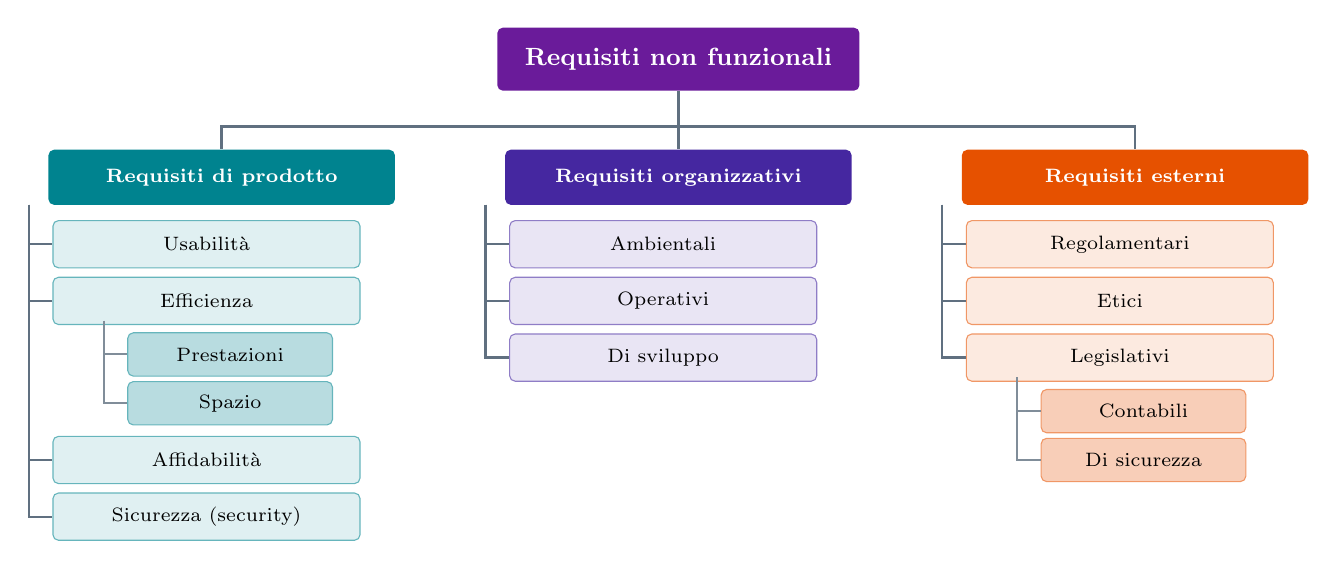
\begin{tikzpicture}[font=\scriptsize,
  figlio/.style 2 args={subchip=#1, minimum width=3.9cm, minimum height=0.6cm, anchor=west, text width=3.5cm, align=center},
  nipote/.style 2 args={subchip=#1, fill=#1!28, minimum width=2.6cm, minimum height=0.55cm, anchor=west}]

  \node[chip=ph3, minimum width=4.6cm, minimum height=0.8cm, font=\small\bfseries] (root) at (0,0) {Requisiti non funzionali};

  % --- le tre famiglie
  \node[chip=q3, minimum width=4.4cm, minimum height=0.7cm, font=\scriptsize\bfseries] (prod) at (-5.8,-1.5) {Requisiti di prodotto};
  \node[chip=q7, minimum width=4.4cm, minimum height=0.7cm, font=\scriptsize\bfseries] (org)  at (0,-1.5)    {Requisiti organizzativi};
  \node[chip=q5, minimum width=4.4cm, minimum height=0.7cm, font=\scriptsize\bfseries] (ext)  at (5.8,-1.5)  {Requisiti esterni};
  \foreach \n in {prod,org,ext}{ \draw[line width=0.9pt, swgray] (root.south) -- ++(0,-0.45) -| (\n.north); }

  % --- colonna PRODOTTO (binario a x=-8.25, figli con anchor west a x=-7.95)
  \node[figlio={q3}{}] (fu) at (-7.95,-2.35) {Usabilità};
  \node[figlio={q3}{}] (fe) at (-7.95,-3.07) {Efficienza};
  \node[figlio={q3}{}] (fa) at (-7.95,-5.09) {Affidabilità};
  \node[figlio={q3}{}] (fs) at (-7.95,-5.81) {Sicurezza (security)};
  \draw[line width=0.8pt, swgray] (-8.25,-1.85) -- (-8.25,-5.81);
  \foreach \n in {fu,fe,fa,fs}{ \draw[line width=0.8pt, swgray] (-8.25,-1.85) |- (\n.west); }
  % sotto-figli di Efficienza (binario indentato a x=-7.3)
  \node[nipote={q3}{}] (np) at (-7.0,-3.75) {Prestazioni};
  \node[nipote={q3}{}] (ns) at (-7.0,-4.37) {Spazio};
  \draw[line width=0.7pt, swgray!80] (-7.3,-3.32) -- (-7.3,-4.37);
  \foreach \n in {np,ns}{ \draw[line width=0.7pt, swgray!80] (-7.3,-3.37) |- (\n.west); }

  % --- colonna ORGANIZZATIVI
  \node[figlio={q7}{}] (oa) at (-2.15,-2.35) {Ambientali};
  \node[figlio={q7}{}] (oo) at (-2.15,-3.07) {Operativi};
  \node[figlio={q7}{}] (os) at (-2.15,-3.79) {Di sviluppo};
  \draw[line width=0.8pt, swgray] (-2.45,-1.85) -- (-2.45,-3.79);
  \foreach \n in {oa,oo,os}{ \draw[line width=0.8pt, swgray] (-2.45,-1.85) |- (\n.west); }

  % --- colonna ESTERNI
  \node[figlio={q5}{}] (er) at (3.65,-2.35) {Regolamentari};
  \node[figlio={q5}{}] (ee) at (3.65,-3.07) {Etici};
  \node[figlio={q5}{}] (el) at (3.65,-3.79) {Legislativi};
  \draw[line width=0.8pt, swgray] (3.35,-1.85) -- (3.35,-3.79);
  \foreach \n in {er,ee,el}{ \draw[line width=0.8pt, swgray] (3.35,-1.85) |- (\n.west); }
  % sotto-figli di Legislativi
  \node[nipote={q5}{}] (ec) at (4.6,-4.47) {Contabili};
  \node[nipote={q5}{}] (es) at (4.6,-5.09) {Di sicurezza};
  \draw[line width=0.7pt, swgray!80] (4.3,-4.04) -- (4.3,-5.09);
  \foreach \n in {ec,es}{ \draw[line width=0.7pt, swgray!80] (4.3,-4.09) |- (\n.west); }
\end{tikzpicture}
\caption{Tassonomia dei requisiti non funzionali in base alla loro origine.}
\end{figure}

\begin{table}[H]
\centering
\renewcommand{\arraystretch}{1.4}
\begin{tabularx}{\textwidth}{>{\bfseries}P{3.4cm} L L}
\toprule
Origine & Cosa riguardano & Esempi \\
\midrule
\textcolor{q3}{Di prodotto} & Caratteristiche richieste al prodotto stesso & Velocità del sistema, memoria occupata, usabilità, tasso di guasti accettabile \\
\textcolor{q7}{Organizzativi} & Politiche e procedure dell'organizzazione del cliente o dello sviluppatore & Processi operativi con cui il sistema sarà usato, linguaggio di programmazione obbligatorio, ambiente operativo da rispettare \\
\textcolor{q5}{Esterni} & Fattori esterni al sistema e al processo di sviluppo & Approvazione da parte di un ente regolatore, obblighi di legge, requisiti etici per l'accettabilità da parte di utenti e pubblico \\
\bottomrule
\end{tabularx}
\end{table}

\subsection{Requisiti di dominio}

\dfn{Requisiti di dominio}{
  Requisiti che derivano dallo \textbf{specifico settore o contesto industriale} in cui il software viene usato.
  Possono essere sia funzionali sia non funzionali.
}

\begin{esempio}{Un requisito di dominio per un dispositivo medico}
«La sicurezza del sistema deve essere garantita secondo lo standard IEC 60601-1: \textit{Medical Electrical Equipment --- Part 1:
General Requirements for Basic Safety and Essential Performance}.»

Questo requisito vincola sia la \textbf{progettazione} del sistema sia il \textbf{processo di sviluppo}: un software perfettamente
funzionante ma non sviluppato secondo lo standard \textbf{non potrebbe essere usato} in pratica.
\end{esempio}

\info{Misurare i requisiti non funzionali}{
  Per essere utile, un requisito non funzionale deve essere associato a una \textbf{metrica}:

  \begin{center}
  \renewcommand{\arraystretch}{1.25}
  \begin{tabular}{>{\bfseries}l l}
  \toprule
  Proprietà & Metriche tipiche \\
  \midrule
  Prestazioni & Operazioni elaborate al secondo; tempo di risposta; tempo di aggiornamento dello schermo \\
  Dimensione & Megabyte occupati \\
  Facilità d'uso & Ore di formazione necessarie; tasso di errore degli utenti; richieste di assistenza \\
  Affidabilità & Tempo medio tra due guasti; percentuale di disponibilità \\
  Robustezza & Tempo di ripristino dopo un guasto; probabilità di perdita di dati \\
  \bottomrule
  \end{tabular}
  \end{center}
}

% ============================================================
\section{Le proprietà di un buon requisito}

\begin{table}[H]
\centering
\renewcommand{\arraystretch}{1.45}
\begin{tabularx}{\textwidth}{>{\bfseries\leavevmode\color{ph1}}P{3.2cm} L}
\toprule
Proprietà & Significato \\
\midrule
Chiaro & Facile da capire, soprattutto per i requisiti utente. \\
Non ambiguo & Una sola interpretazione possibile: l'ambiguità porta a \textbf{contenziosi} con il cliente. \\
Completo & Non deve mancare nulla di ciò che serve. \\
Coerente & I requisiti non devono contraddirsi tra loro. \\
Testabile & Dato un requisito, deve essere possibile stabilire \textbf{senza dubbi} se il sistema lo soddisfa. \\
Tracciabile & Deve essere collegabile «in avanti e all'indietro» alle altre parti della documentazione: progetto, codice, test. \\
\bottomrule
\end{tabularx}
\end{table}

\subsection{I demoni dell'ambiguità}

Il linguaggio naturale è comodo ma insidioso. Consideriamo un cartello stradale che tutti capiamo al volo:

\begin{figure}[H]
\centering
\begin{minipage}[c]{0.24\textwidth}
\centering
\begin{tikzpicture}[scale=0.95]
  % cartello "school" (pentagono giallo)
  \fill[yellow-gradient-6!85!black] (-1.0,2.1) -- (1.0,2.1) -- (1.0,3.3) -- (0,3.95) -- (-1.0,3.3) -- cycle;
  \draw[draw=black, line width=1pt] (-1.0,2.1) -- (1.0,2.1) -- (1.0,3.3) -- (0,3.95) -- (-1.0,3.3) -- cycle;
  \node[font=\bfseries\scriptsize, text=black] at (0,2.85) {SCHOOL};
  % cartello del limite di velocita'
  \draw[draw=black, fill=white, line width=1pt] (-1.05,-0.75) rectangle (1.05,1.85);
  \node[font=\tiny\bfseries, text=black, align=center] at (0,1.55) {SPEED\\LIMIT};
  \node[font=\Huge\bfseries, text=black] at (0,0.75) {20};
  \node[font=\tiny\bfseries, text=black, align=center] at (0,-0.3) {WHEN\\CHILDREN\\ARE PRESENT};
  \draw[swgray, line width=2pt] (0,-0.75) -- (0,-1.35);
\end{tikzpicture}
\end{minipage}\hfill
\begin{minipage}[c]{0.72\textwidth}
Per un essere umano l'intento è chiaro: proteggere i bambini in una zona scolastica. Ma proviamo a spiegarlo a un computer:
\begin{itemize}
  \item perché il cartello dice «children» (plurale) e non «child»? La regola vale solo se c'è \textbf{più di un} bambino?
  \item chi è considerato un «bambino»? Un ragazzo di 17 anni lo è?
  \item cosa significa essere «presenti»? Dentro la scuola? Sul marciapiede? Visibili dalla strada?
  \item la regola vale solo quando la scuola è aperta?
\end{itemize}
\end{minipage}
\caption{Un cartello chiarissimo per una persona, pieno di ambiguità per una macchina (H. Robinson, \textit{The demons of ambiguity}).}
\end{figure}

\begin{esempio}{Le domande nascoste in un requisito}
Requisito: \textit{«L'applicazione deve permettere agli utenti di avviare e arrestare un servizio su una macchina remota.»}

Sembra chiaro, ma:
\begin{itemize}
  \item cosa succede se si avvia un servizio \textbf{già in esecuzione}? E se si arresta un servizio \textbf{non in esecuzione}?
  \item se la macchina remota si \textbf{riavvia}, il servizio deve ripartire automaticamente?
  \item se cade la \textbf{connessione}: l'applicazione mostra un messaggio d'errore? Riprova? Dopo quanto tempo?
        Quanti tentativi al massimo?
\end{itemize}
Ognuna di queste domande, se non trova risposta nei requisiti, diventerà una discussione (o un contenzioso) con il cliente.
\end{esempio}

\subsection{Testabilità}

Deve essere possibile stabilire \textbf{senza ambiguità} se il sistema soddisfa un requisito: altrimenti gli sviluppatori
sosterranno che il requisito è soddisfatto e il cliente sosterrà il contrario. In pratica:

\begin{itemize}
  \item i requisiti \textbf{funzionali di sistema} devono essere il più dettagliati possibile e non lasciare spazio a interpretazioni;
  \item i requisiti \textbf{non funzionali} devono includere, quando possibile, \textbf{indicatori quantitativi}.
\end{itemize}

\begin{table}[H]
\centering
\renewcommand{\arraystretch}{1.45}
\begin{tabularx}{\textwidth}{L L}
\toprule
\textcolor{swred}{\textbf{\icross\ Poco testabile}} & \textcolor{swgreen}{\textbf{\itick\ Testabile}} \\
\midrule
Il sistema deve essere affidabile. & Il sistema deve avere una disponibilità mensile del 99,99\%. \\
Il sistema deve essere facile da usare. & Dopo al più due ore di formazione, gli utenti devono saper usare tutte le funzioni del sistema; dopo la formazione, il numero medio di errori non deve superare i due per ora di utilizzo. \\
Il sistema deve essere veloce e reattivo. & Il tempo medio di risposta del sistema non deve superare i 100 ms. \\
\bottomrule
\end{tabularx}
\caption{Trasformare requisiti vaghi in requisiti verificabili.}
\end{table}

% ============================================================
\section{Il processo di Requirements Engineering}

Il processo di RE si articola in tre attività principali.

\begin{figure}[H]
\centering
\begin{tikzpicture}
  \node[phase=ph1, minimum width=4.2cm, minimum height=1.2cm, font=\small\bfseries, drop shadow] (el) at (0,0) {Elicitazione\\e analisi};
  \node[phase=ph3, minimum width=4.2cm, minimum height=1.2cm, font=\small\bfseries, drop shadow] (sp) at (5.9,0) {Specifica};
  \node[phase=ph5, minimum width=4.2cm, minimum height=1.2cm, font=\small\bfseries, drop shadow] (va) at (11.8,0) {Validazione};
  \draw[flow] (el) -- (sp);
  \draw[flow] (sp) -- (va);
  \draw[feedback] (va.north) to[out=120, in=60] node[above, font=\scriptsize, text=swred]{i problemi trovati fanno tornare indietro} (el.north);
  \node[card=ph1, text width=4.2cm, font=\scriptsize, align=left, below=0.5cm of el] (d1) {\textbf{Scopo}: scoprire i requisiti interagendo con gli stakeholder.\\[3pt]\textit{Output}: descrizione del sistema.};
  \node[card=ph3, text width=4.2cm, font=\scriptsize, align=left, below=0.5cm of sp] (d2) {\textbf{Scopo}: convertire i requisiti in una forma standardizzata.\\[3pt]\textit{Output}: requisiti utente e di sistema.};
  \node[card=ph5, text width=4.2cm, font=\scriptsize, align=left, below=0.5cm of va] (d3) {\textbf{Scopo}: controllare che i requisiti definiscano davvero il sistema voluto dal cliente.\\[3pt]\textit{Output}: documento dei requisiti.};
\end{tikzpicture}
\caption{Le tre attività del processo di Requirements Engineering.}
\end{figure}

\subsection{Un processo iterativo, non lineare}

Nella pratica queste attività non si susseguono una sola volta: si \textbf{intrecciano} in un processo iterativo che lavora
a \textbf{livelli di granularità} diversi.

\begin{enumerate}
  \item Nella prima iterazione ci si concentra sui \textbf{requisiti di business}: perché il progetto è necessario?
        Chi ne beneficia? Quando e dove verrà usato?
  \item Poi si definiscono i \textbf{requisiti utente}.
  \item Infine si definiscono i \textbf{requisiti di sistema}.
\end{enumerate}

Ogni iterazione comprende elicitazione e analisi, specifica e validazione.

\begin{figure}[H]
\centering
\begin{tikzpicture}[font=\scriptsize]
  \foreach \c/\tit/\x in {0/{Elicitazione / Analisi}/0, 1/{Specifica}/5.3, 2/{Validazione}/10.6}{
    \node[font=\small\bfseries, text=swgray] at (\x,1.1) {\tit};
  }
  \foreach \r/\liv/\col/\val/\y in {0/{Business}/q1/{Studio di fattibilità}/0,
                                    1/{Utente}/q4/{Prototipazione}/-1.8,
                                    2/{Sistema}/q2/{Revisione}/-3.6}{
    \node[phase=\col, minimum width=4.4cm, minimum height=1.1cm, font=\scriptsize\bfseries] (a\r) at (0,\y) {Elicitazione e analisi\\dei requisiti \liv};
    \node[phase=\col, minimum width=4.4cm, minimum height=1.1cm, font=\scriptsize\bfseries] (b\r) at (5.3,\y) {Specifica dei requisiti\\\liv};
    \node[phase=\col, fill=\col!70, minimum width=4.4cm, minimum height=1.1cm, font=\scriptsize\bfseries] (c\r) at (10.6,\y) {\val};
    \node[card=\col, minimum width=2.4cm, minimum height=1.1cm, font=\scriptsize\bfseries, anchor=west] (d\r) at (13.3,\y) {Requisiti\\\liv};
    \draw[flow] (a\r) -- (b\r);
    \draw[flow] (b\r) -- (c\r);
    \draw[flow] (c\r) -- (d\r);
  }
  \foreach \r [evaluate=\r as \s using int(\r+1)] in {0,1}{
    \draw[-{Stealth[length=2.5mm]}, line width=1pt, swgray] (d\r.south) -- ++(0,-0.35) -| ([xshift=-0.55cm]a\s.north west) -- ([xshift=-0.02cm]a\s.west);
  }
\end{tikzpicture}
\caption{Il processo iterativo: ogni livello di requisiti attraversa le tre attività e alimenta il livello successivo.}
\end{figure}

% ============================================================
\section{Elicitazione e analisi dei requisiti}

\dfn{Elicitazione dei requisiti}{
  Attività il cui obiettivo è \textbf{scoprire che cosa i clienti vogliono e di cosa hanno bisogno}, interagendo con gli
  stakeholder. È considerata la parte \textbf{più critica} dell'intera ingegneria dei requisiti.
}

Detta così sembra banale; in realtà è la parte più difficile del mestiere, per un motivo semplice: le persone non sanno
sempre cosa vogliono, e quasi mai lo sanno spiegare in termini utilizzabili da chi deve costruire il software.

\subsection{Chi sono gli stakeholder}

\dfn{Stakeholder}{
  Le \textbf{persone o i gruppi} che sono in qualche modo interessati o influenzati dal progetto software.
}

\begin{figure}[H]
\centering
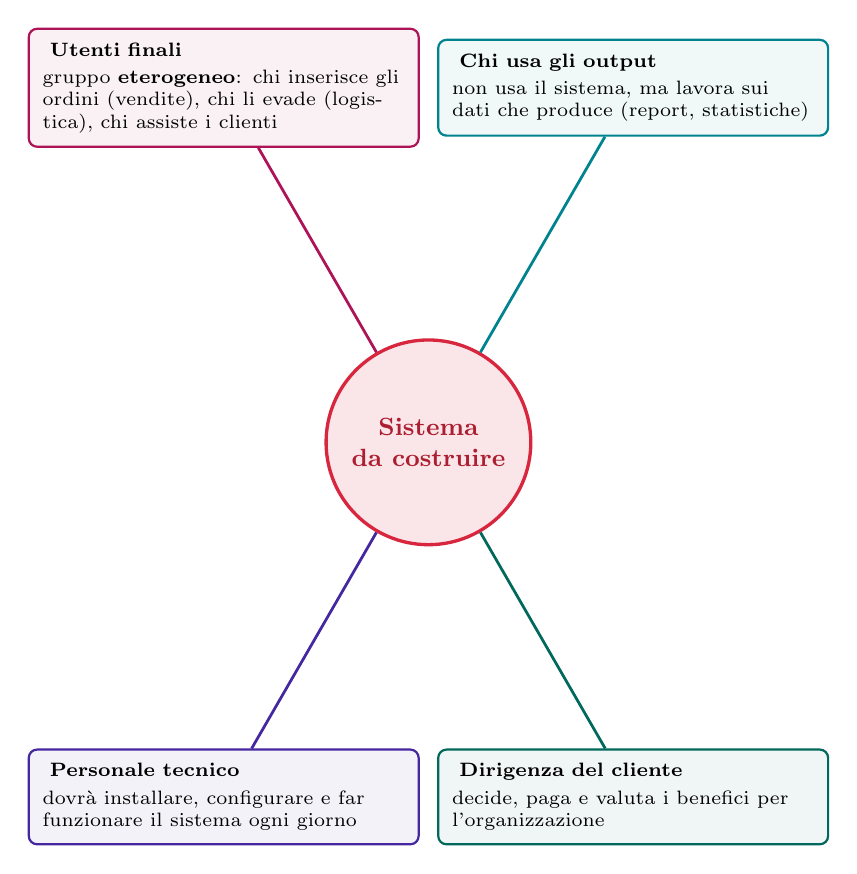
\begin{tikzpicture}
  \node[circle, fill=ph1!12, draw=ph1, line width=1.2pt, minimum size=2.6cm, align=center, font=\small\bfseries, text=ph1!80!black] (sys) at (0,0) {Sistema\\da costruire};
  \foreach \ang/\tit/\desc/\col in {
      120/{Utenti finali}/{gruppo \textbf{eterogeneo}: chi inserisce gli ordini (vendite), chi li evade (logistica), chi assiste i clienti}/q4,
      60/{Chi usa gli output}/{non usa il sistema, ma lavora sui dati che produce (report, statistiche)}/q3,
      -60/{Dirigenza del cliente}/{decide, paga e valuta i benefici per l'organizzazione}/q1,
      -120/{Personale tecnico}/{dovrà installare, configurare e far funzionare il sistema ogni giorno}/q7}{
    \node[card=\col, text width=4.6cm, font=\scriptsize, align=left] (n\ang) at (\ang:5.2) {\textbf{\iuser\ \tit}\\[2pt]\desc};
    \draw[line width=1pt, \col] (sys) -- (n\ang);
  }
\end{tikzpicture}
\caption{Gli stakeholder tipici di un sistema di gestione degli ordini.}
\end{figure}

\subsection{Perché è difficile}

\begin{figure}[H]
\centering
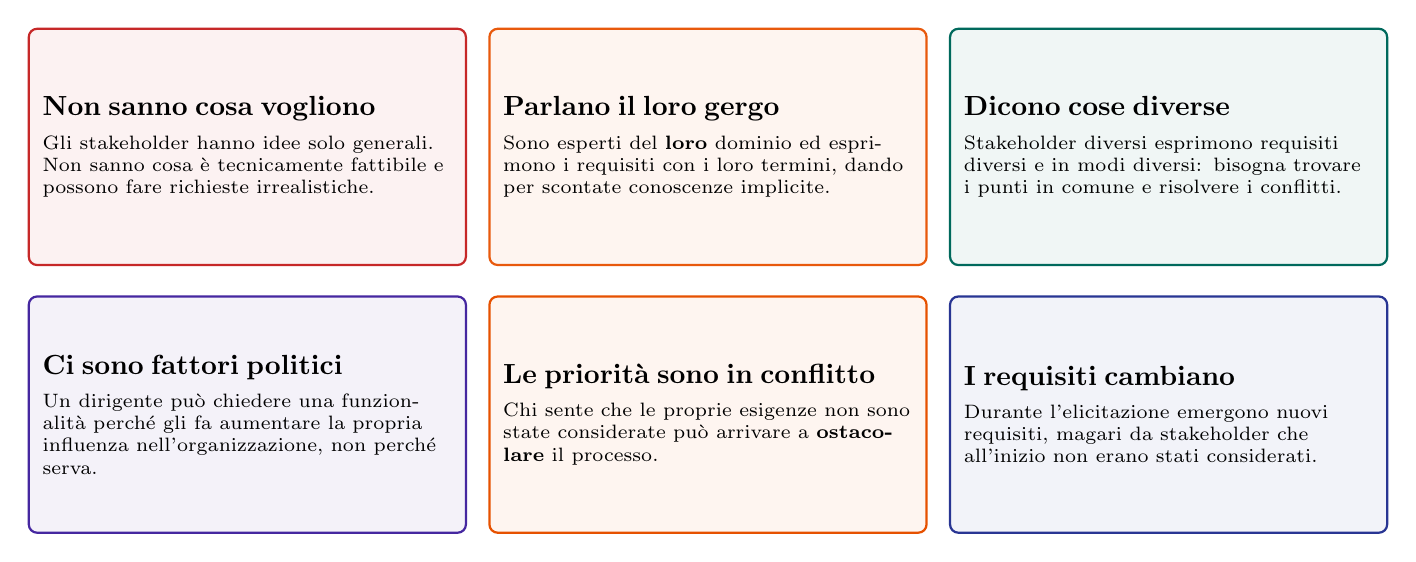
\begin{tikzpicture}
  \foreach \i/\tit/\txt/\col in {
    0/{Non sanno cosa vogliono}/{Gli stakeholder hanno idee solo generali. Non sanno cosa è tecnicamente fattibile e possono fare richieste irrealistiche.}/swred,
    1/{Parlano il loro gergo}/{Sono esperti del \textbf{loro} dominio ed esprimono i requisiti con i loro termini, dando per scontate conoscenze implicite.}/sworange,
    2/{Dicono cose diverse}/{Stakeholder diversi esprimono requisiti diversi e in modi diversi: bisogna trovare i punti in comune e risolvere i conflitti.}/q1}{
    \node[card=\col, text width=5.2cm, minimum height=3.0cm, align=left, font=\scriptsize, anchor=north west] at (\i*5.85,0) {\textbf{\normalsize\tit}\\[4pt]\txt};
  }
  \foreach \i/\tit/\txt/\col in {
    0/{Ci sono fattori politici}/{Un dirigente può chiedere una funzionalità perché gli fa aumentare la propria influenza nell'organizzazione, non perché serva.}/q7,
    1/{Le priorità sono in conflitto}/{Chi sente che le proprie esigenze non sono state considerate può arrivare a \textbf{ostacolare} il processo.}/q5,
    2/{I requisiti cambiano}/{Durante l'elicitazione emergono nuovi requisiti, magari da stakeholder che all'inizio non erano stati considerati.}/q2}{
    \node[card=\col, text width=5.2cm, minimum height=3.0cm, align=left, font=\scriptsize, anchor=north west] at (\i*5.85,-3.4) {\textbf{\normalsize\tit}\\[4pt]\txt};
  }
\end{tikzpicture}
\caption{Le sei principali difficoltà dell'elicitazione dei requisiti.}
\end{figure}

\subsection{Il processo di elicitazione e analisi}

L'attività si svolge come un \textbf{ciclo} che si ripete finché i requisiti non sono sufficientemente stabili.

\begin{figure}[H]
\centering
\begin{tikzpicture}
  \node[phase=ph1, minimum width=3.9cm, minimum height=1.1cm, font=\scriptsize\bfseries] (d1) at (0,2.3) {1. Scoperta e\\comprensione};
  \node[phase=ph2, minimum width=3.9cm, minimum height=1.1cm, font=\scriptsize\bfseries] (d2) at (4.3,0) {2. Classificazione\\e organizzazione};
  \node[phase=ph4, minimum width=3.9cm, minimum height=1.1cm, font=\scriptsize\bfseries] (d3) at (0,-2.3) {3. Prioritizzazione\\e negoziazione};
  \node[phase=ph6, minimum width=3.9cm, minimum height=1.1cm, font=\scriptsize\bfseries] (d4) at (-4.3,0) {4. Documentazione};
  \node[font=\scriptsize\itshape, text=swgray, align=center] at (0,0) {il ciclo si ripete\\finché i requisiti\\non sono stabili};
  \draw[flow, line width=1.4pt] (d1) to[out=0, in=90] (d2);
  \draw[flow, line width=1.4pt] (d2) to[out=270, in=0] (d3);
  \draw[flow, line width=1.4pt] (d3) to[out=180, in=270] (d4);
  \draw[flow, line width=1.4pt] (d4) to[out=90, in=180] (d1);
\end{tikzpicture}
\caption{Il ciclo di elicitazione e analisi dei requisiti.}
\end{figure}

\begin{table}[H]
\centering
\renewcommand{\arraystretch}{1.35}
\begin{tabularx}{\textwidth}{>{\bfseries}P{5.0cm} L}
\toprule
\textcolor{ph1}{1. Scoperta e comprensione} & Si interagisce con gli stakeholder per \textbf{scoprire} i requisiti. \\
\textcolor{ph2}{2. Classificazione e organizzazione} & I requisiti correlati vengono \textbf{raggruppati} e organizzati in categorie coerenti. \\
\textcolor{ph4}{3. Prioritizzazione e negoziazione} & Si risolvono i \textbf{conflitti} che nascono dalle esigenze contrastanti dei diversi stakeholder. \\
\textcolor{ph6}{4. Documentazione} & I requisiti trovati vengono \textbf{documentati}, come base per l'iterazione successiva. \\
\bottomrule
\end{tabularx}
\end{table}

% ============================================================
\section{Le tecniche di elicitazione}

Non esiste una tecnica unica: si combinano approcci diversi.

\begin{center}
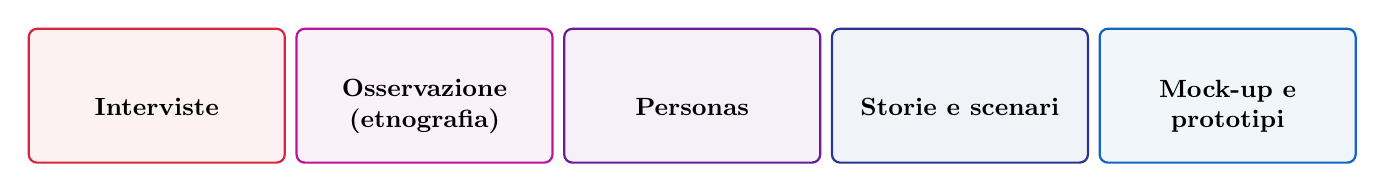
\begin{tikzpicture}
  \foreach \i/\tit/\ico/\col in {0/{Interviste}/\iuser/ph1, 1/{Osservazione\\(etnografia)}/\ieye/ph2, 2/{Personas}/\ibadge/ph3,
                                 3/{Storie e scenari}/\ibook/ph4, 4/{Mock-up e\\prototipi}/\iwindow/ph5}{
    \node[card=\col, text width=2.9cm, minimum height=1.7cm, align=center, font=\small\bfseries] at (\i*3.4,0) {{\Large\ico}\\[3pt]\tit};
  }
\end{tikzpicture}
\end{center}

% ------------------------------------------------------------
\subsection{Interviste con gli stakeholder}

Le interviste, formali o informali, sono lo strumento fondamentale della RE: il team chiede agli stakeholder come lavorano,
quale sistema usano oggi e cosa si aspettano dal sistema da sviluppare. I requisiti si ricavano dalle risposte.

\begin{table}[H]
\centering
\renewcommand{\arraystretch}{1.4}
\begin{tabularx}{\textwidth}{>{\bfseries}P{3.4cm} L}
\toprule
Intervista chiusa & Lo stakeholder risponde a una \textbf{lista di domande predefinita}. \\
Intervista aperta & Non c'è un'agenda prestabilita: si lascia parlare l'intervistato. \\
\midrule
\textcolor{swgreen}{\textbf{In pratica}} & Si usa una \textbf{combinazione} delle due. Le interviste completamente aperte funzionano raramente: conviene partire da un insieme di domande preparate, che di solito portano ad altri temi da discutere in modo meno strutturato. \\
\bottomrule
\end{tabularx}
\end{table}

\begin{center}
\begin{tikzpicture}
  \node[card=swgreen, text width=7.7cm, minimum height=2.6cm, align=left, font=\small] (pro) {%
    \textbf{\itick\ Il lato buono}\\[3pt]\scriptsize
    Alle persone in genere piace parlare del proprio lavoro e partecipano alle interviste con un atteggiamento positivo.};
  \node[card=swred, text width=7.7cm, minimum height=2.6cm, align=left, font=\small, right=0.4cm of pro] (con) {%
    \textbf{\icross\ Le difficoltà}\\[3pt]\scriptsize
    \textbullet\ usano \textbf{gergo} tecnico e danno per scontati molti requisiti;\\
    \textbullet\ conoscono bene il \textbf{proprio} lavoro, ma hanno una visione parziale o distorta di quello dei colleghi di altri reparti;\\
    \textbullet\ possono essere \textbf{reticenti} su vincoli organizzativi, per via di equilibri di potere interni.};
\end{tikzpicture}
\end{center}

\warning{Rispettare il tempo degli stakeholder}{
  Gli stakeholder hanno il loro lavoro da fare: le interviste vanno preparate bene, per non sprecare il loro tempo
  (e il nostro) con riunioni inutili.
}

\begin{esempio}{Il gergo: una storia vera}
Durante un tirocinio presso la direzione finanziaria di un grande Comune, un tributo minore veniva gestito quasi interamente
con fogli di calcolo. Alla domanda «mi racconta come funziona la gestione di questo tributo?», la risposta è stata:

\begin{center}
\begin{tcolorbox}[enhanced, breakable=false, colback=swteal!8, colframe=swteal, boxrule=0.8pt, arc=3pt, width=0.95\linewidth, fontupper=\itshape\small]
  «Certo! È molto semplice! Un operatore sul campo mi invia la \textbf{lettura} per un dato anno per un certo contribuente.
  Quindi inserisco la lettura in una maschera che calcola l'\textbf{imponibile}. Successivamente faccio la stampa delle
  \textbf{ingiunzioni di pagamento}, che vengono poi emesse. Una volta notificata l'ingiunzione, il contribuente ha 60 giorni
  per pagare. Se non paga entro il termine, devo procedere all'\textbf{iscrizione al ruolo coattivo}: inserisco i dati in una
  maschera che genera il \textbf{Tracciato 290} da trasmettere all'ente di riscossione.»
\end{tcolorbox}
\end{center}

«È molto semplice» --- ma per capire davvero quella frase servono settimane di studio del dominio. Questo è esattamente il
problema del gergo: per l'intervistato è ovvio, per l'ingegnere del software è una lingua straniera. Il lavoro consiste nel
farsi spiegare ogni termine, finché la descrizione non diventa un insieme di requisiti precisi.
\end{esempio}

% ------------------------------------------------------------
\subsection{Etnografia}

\dfn{Etnografia}{
  Tecnica \textbf{osservativa} in cui l'ingegnere dei requisiti si \textbf{immerge nell'ambiente di lavoro} degli utenti finali:
  osserva il lavoro quotidiano e prende nota dei compiti realmente svolti e delle persone coinvolte.
}

Il software non vive isolato: è usato in un ambiente \textbf{sociale e organizzativo} che può generare o vincolare requisiti.
E, molto spesso, il modo in cui si lavora davvero è \textbf{diverso} dal processo formale che si dovrebbe seguire.

L'etnografia è particolarmente efficace per scoprire:
\begin{itemize}
  \item requisiti che derivano dal modo in cui le persone \textbf{lavorano realmente}, invece che dal modo in cui le procedure
        aziendali dicono che dovrebbero lavorare;
  \item requisiti che derivano dalla \textbf{cooperazione} e dalla consapevolezza delle attività altrui.
\end{itemize}

\begin{esempio}{Un requisito che nessuno avrebbe raccontato}
Osservando l'ufficio, si nota che prima di inviare un questionario di soddisfazione al cliente, un addetto del servizio clienti
telefona ogni volta a un collega della logistica per sapere se l'ordine è stato davvero consegnato.

Nessuno lo avrebbe mai detto in un'intervista («si fa così e basta»), ma da lì nasce un requisito preciso:
\textit{«Gli addetti al servizio clienti devono poter verificare se un cliente ha già ricevuto il proprio ordine.»}
\end{esempio}

% ------------------------------------------------------------
\subsection{Personas}

\dfn{Persona}{
  Un \textbf{archetipo ipotetico} di utente reale. Le \textit{personas} non sono persone vere, ma le rappresentano:
  sono immaginarie, eppure definite con \textbf{rigore e precisione}, e non sono inventate di sana pianta, ma \textbf{scoperte}
  come sottoprodotto del processo di elicitazione.
}

Conoscere l'utente è fondamentale sia per scoprire i requisiti sia (lo vedremo più avanti) per progettare interfacce efficaci.
A volte gli utenti li conosciamo bene (ad esempio se sviluppiamo uno strumento per altri ingegneri del software), ma in generale
il software è fatto \textbf{per altre persone}, con esigenze diverse dalle nostre: la nostra esperienza personale non basta
a immaginare come lavorano e cosa vogliono.

Le personas servono anche quando \textbf{non abbiamo stakeholder da intervistare}: ad esempio quando sviluppiamo un prodotto
generico per il grande pubblico, o quando parte degli utenti finali è il pubblico generico.

Non esiste un formato standard; di solito una persona contiene:

\begin{center}
\begin{tikzpicture}
  \foreach \i/\t/\d in {0/{Personalizzazione}/{nome, età, breve biografia},
                        1/{Lavoro}/{che lavoro fa?},
                        2/{Istruzione}/{studi ed esperienza},
                        3/{Obiettivi}/{cosa si aspetta dal software?},
                        4/{Frustrazioni}/{quali problemi il software può risolverle?}}{
    \node[card=ph3, text width=2.8cm, minimum height=1.6cm, align=center, font=\scriptsize] at (\i*3.25,0) {\textbf{\t}\\[3pt]\d};
  }
\end{tikzpicture}
\end{center}

\begin{esempio}{Una persona per un gestionale di studio dentistico}
Supponiamo di raccogliere i requisiti per un software di gestione degli appuntamenti di uno studio dentistico.
Intervistando il personale abbiamo già ricavato alcuni requisiti:
\begin{itemize}\itemsep1pt
  \item i pazienti devono potersi registrare e autenticare nel sistema;
  \item i pazienti devono poter prenotare un appuntamento in uno slot libero;
  \item i medici devono poter vedere gli appuntamenti della settimana corrente;
  \item i receptionist devono poter cancellare gli appuntamenti;
  \item i pazienti devono ricevere un promemoria via e-mail il giorno prima dell'appuntamento;
  \item i pazienti devono ricevere un'e-mail se il loro appuntamento viene annullato.
\end{itemize}

Costruiamo ora una persona:

\begin{center}
\begin{tcolorbox}[enhanced, breakable=false, colback=white, colframe=ph3, boxrule=1pt, arc=3pt, drop fuzzy shadow,
   width=\linewidth, left=6pt, right=6pt]
\begin{minipage}[t]{0.30\linewidth}
  \centering
  \begin{tikzpicture}
    \fill[ph3!15, rounded corners=4pt] (-1.3,-1.5) rectangle (1.3,1.5);
    \fill[ph3!55] (0,0.55) circle (0.45);
    \fill[ph3!55] (-0.75,-1.2) .. controls (-0.75,0.05) and (0.75,0.05) .. (0.75,-1.2) -- cycle;
  \end{tikzpicture}\\[4pt]
  {\small\textbf{Concetta (Tina) Aiello}}\\[2pt]
  {\scriptsize Età: 68 --- vedova\\ Pensionata (ex maestra elementare)\\ \textit{assertiva, impaziente}}
\end{minipage}\hfill
\begin{minipage}[t]{0.66\linewidth}
  \small\textbf{Bio.} Tina è un'insegnante di scuola primaria in pensione, con oltre 40 anni di esperienza. È dolce e paziente
  con i bambini, ma diventa impaziente quando si trova fuori dalla sua zona di comfort. Ama la sua routine quotidiana e non
  le piace cambiarla. La tecnologia non le piace: l'anno scorso i figli le hanno regalato il primo smartphone, che usa solo per
  videochiamare le nipoti. È diffidente verso internet, che percepisce come un posto pericoloso.\\[3pt]
  \textbf{Interessi.} Lavoro a maglia; comunità della parrocchia; tempo con le nipoti.\\[3pt]
  \textbf{Obiettivi.} Prenotare i controlli periodici della protesi dentale; ricevere un promemoria per non dimenticare
  l'appuntamento; spostare un appuntamento se coincide con un altro impegno.
\end{minipage}
\end{tcolorbox}
\end{center}

\textbf{Cosa abbiamo scoperto.} Tina non prenoterà mai da sola tramite l'app: telefonerà allo studio. E un promemoria via e-mail
non lo leggerà. Nascono quindi \textbf{nuovi requisiti} che nessuno aveva pensato di dirci:
\begin{itemize}\itemsep1pt
  \item i receptionist devono poter creare appuntamenti per i pazienti che telefonano allo studio;
  \item il giorno prima dell'appuntamento, i receptionist devono ricevere una notifica che ricordi loro di \textbf{telefonare}
        ai pazienti che hanno prenotato per telefono.
\end{itemize}
\end{esempio}

% ------------------------------------------------------------
\subsection{Storie e scenari}

\dfn{Storia (story)}{
  Testo \textbf{narrativo} che presenta una descrizione ad alto livello dell'uso del sistema. È efficace per comunicare
  gli obiettivi «di insieme» in modo comprensibile a chiunque.
}

\begin{center}
\begin{tcolorbox}[enhanced, breakable=false, colback=ph4!5, colframe=ph4, boxrule=0.9pt, arc=3pt,
  title={\textbf{Storia: prenotare un appuntamento con l'app}}, coltitle=white, colbacktitle=ph4, fontupper=\small]
  Pamela ha bisogno di prenotare una visita odontoiatrica perché il dente del giudizio ha iniziato a farle male.
  Accede al sistema e cerca gli slot disponibili per oggi o per domani. Il sistema mostra l'elenco degli slot liberi.
  Pamela ne sceglie uno e conferma la prenotazione. Riceve un'e-mail di conferma con i dettagli dell'appuntamento.
\end{tcolorbox}
\end{center}

\dfn{Scenario}{
  Descrizione (tipicamente \textbf{strutturata}) di un esempio di interazione tra utente e sistema. Raffina una storia
  aggiungendo informazioni precise: stato iniziale, flusso normale degli eventi, cosa può andare storto e come si gestisce,
  altre attività in corso nello stesso momento, stato del sistema alla fine.
}

\begin{table}[H]
\centering
\renewcommand{\arraystretch}{1.4}
\begin{tabularx}{\textwidth}{>{\bfseries\leavevmode\color{ph4}}P{3.4cm} L}
\toprule
\multicolumn{2}{l}{\textcolor{ph4}{\textbf{Scenario: prenotazione di un appuntamento}}} \\
\midrule
Assunzioni iniziali & L'utente ha un account sul sistema di gestione degli appuntamenti. \\
Flusso normale & L'utente effettua il login e cerca gli slot disponibili per la data odierna o per il giorno successivo.
Il sistema mostra l'elenco degli slot liberi nelle date scelte. L'utente seleziona uno degli slot proposti.
Il sistema invia un'e-mail di conferma all'utente, al receptionist e al medico. \\
Cosa può andare storto & \textbullet\ Non c'è nessuno slot disponibile nelle date considerate: il sistema mostra un messaggio
di errore e chiede di scegliere date diverse.\newline
\textbullet\ Lo slot scelto non è più disponibile al momento della conferma, perché un altro utente lo ha prenotato:
il sistema mostra un messaggio di errore e torna alla schermata degli slot disponibili. \\
Stato finale del sistema & Il sistema ha memorizzato il nuovo appuntamento. \\
\bottomrule
\end{tabularx}
\caption{Uno scenario strutturato che raffina la storia precedente.}
\end{table}

% ------------------------------------------------------------
\subsection{Mock-up a bassa fedeltà}

\dfn{Mock-up a bassa fedeltà (wireframe)}{
  \textbf{Schizzi semplificati} delle interfacce utente del sistema. Sono un modo rapido ed economico per visualizzare
  la struttura e i flussi principali: l'attenzione è sulla \textbf{funzionalità e sul flusso}, non sull'estetica.
}

\begin{figure}[H]
\centering
\begin{minipage}[c]{0.46\textwidth}
\centering
\begin{tikzpicture}[line width=0.9pt]
  % schermata 1
  \draw[swgray, rounded corners=3pt] (0,0) rectangle (4.2,5.4);
  \draw[swgray] (0,4.7) -- (4.2,4.7);
  \node[font=\scriptsize\bfseries, text=swgray] at (2.1,5.05) {Prenota una visita};
  \node[font=\tiny, text=swgray, anchor=west] at (0.25,4.25) {Data};
  \draw[swgray!70] (0.25,3.5) rectangle (3.95,4.0);
  \node[font=\tiny, text=swgray!80, anchor=west] at (0.35,3.75) {gg / mm / aaaa};
  \node[font=\tiny, text=swgray, anchor=west] at (0.25,3.15) {Slot disponibili};
  \foreach \k in {0,1,2}{
    \draw[swgray!70] (0.25,2.25-\k*0.65) rectangle (3.95,2.8-\k*0.65);
    \node[font=\tiny, text=swgray!90, anchor=west] at (0.4,2.52-\k*0.65) {0\the\numexpr9+\k\relax:00 --- Dott. Bianchi};
    \draw[swgray!70] (3.35,2.35-\k*0.65) rectangle (3.85,2.7-\k*0.65);
  }
  \draw[fill=swgray!25, swgray, rounded corners=2pt] (1.1,0.35) rectangle (3.1,0.9);
  \node[font=\tiny\bfseries, text=swgray] at (2.1,0.62) {CONFERMA};
\end{tikzpicture}
\end{minipage}\hfill
\begin{minipage}[c]{0.50\textwidth}
\textbf{Perché servono}
\begin{itemize}\itemsep2pt
  \item \textbf{Facilitano la comprensione}: aiutano gli stakeholder a cogliere le funzionalità di base e sono un punto di
        partenza per la discussione.
  \item \textbf{Fanno scoprire nuovi requisiti}: è molto più facile ragionare su un'interfaccia concreta che su frasi astratte.
  \item \textbf{Coinvolgono e permettono di iterare}: si ottiene feedback rapido senza investire in grafica.
  \item \textbf{Sono una base per lo sviluppo}: da qui si passa ai prototipi ad alta fedeltà e poi all'implementazione.
\end{itemize}
\end{minipage}
\caption{Un wireframe non deve essere bello: deve far capire struttura e flusso.}
\end{figure}

\info{Strumenti}{
  \textbf{Carta e matita}: rapidi e accessibili per i primi schizzi, ma diventano disordinati per sistemi complessi.\\
  \textbf{Strumenti digitali}: software commerciali come \textit{Balsamiq} o \textit{Figma} permettono di creare e condividere
  wireframe elettronicamente; esistono anche alternative open source come \textit{mydraft.cc}, \textit{draw.io} o \textit{Pencil Project}.
}

% ============================================================
\section{La specifica dei requisiti}

\dfn{Specifica dei requisiti}{
  Il processo di \textbf{mettere per iscritto} i requisiti utente e di sistema in un \textbf{documento dei requisiti}.
  I requisiti utente devono essere comprensibili a utenti e clienti senza background tecnico; i requisiti di sistema sono
  più dettagliati e possono contenere informazioni tecniche.
}

Poiché il documento dei requisiti può diventare \textbf{parte del contratto} di sviluppo, è importante che sia il più
completo e dettagliato possibile.

\warning{Requisiti e progetto sono inseparabili}{
  In linea di principio i requisiti dicono \textit{cosa} il sistema deve fare e il progetto dice \textit{come} lo fa.
  In pratica i due aspetti si intrecciano:
  \begin{itemize}
    \item i requisiti possono essere \textbf{organizzati} seguendo un'architettura di sistema di alto livello;
    \item il sistema può dover \textbf{interoperare} con altri sistemi, e questo genera requisiti di progetto;
    \item l'uso di una specifica architettura per soddisfare requisiti non funzionali può essere esso stesso un requisito di dominio.
  \end{itemize}
}

\subsection{Quattro approcci alla specifica}

\begin{figure}[H]
\centering
\begin{tikzpicture}
  \draw[-{Stealth[length=3mm]}, line width=1.2pt, swgray] (-0.4,-0.9) -- (15.6,-0.9) node[right, font=\scriptsize, align=left]{};
  \node[font=\scriptsize, text=swgray] at (7.6,-1.35) {formalità e precisione crescenti $\longrightarrow$};
  \foreach \i/\tit/\txt/\col in {
    0/{Linguaggio naturale}/{Frasi numerate in linguaggio naturale: una frase, un requisito.}/q4,
    1/{Linguaggio naturale strutturato}/{Si usa un \textbf{modulo standard} o un template per ogni requisito.}/q1,
    2/{Notazioni semi-formali}/{Modelli UML (es.\ diagrammi dei casi d'uso) e modelli di dominio, con annotazioni testuali.}/q2,
    3/{Specifica formale}/{Notazioni basate su concetti matematici: automi a stati finiti, logiche temporali.}/q7}{
    \node[card=\col, text width=3.3cm, minimum height=2.7cm, align=left, font=\scriptsize, anchor=south west] at (\i*4.0,-0.7) {\textbf{\small\tit}\\[4pt]\txt};
  }
\end{tikzpicture}
\caption{Dal testo libero alla matematica: quattro modi di specificare i requisiti.}
\end{figure}

Approcci diversi si adattano a domini diversi:

\begin{table}[H]
\centering
\renewcommand{\arraystretch}{1.4}
\begin{tabularx}{\textwidth}{>{\bfseries}P{5.2cm} L}
\toprule
Contesto & Approccio tipico \\
\midrule
Sistemi critici per la sicurezza & Specifiche \textbf{formali} e linguaggio naturale strutturato \\
Una semplice app per le liste di cose da fare & Linguaggio naturale non strutturato \\
Un sistema informativo di media o grande dimensione & Notazioni \textbf{semi-formali} e modelli: un buon compromesso \\
\bottomrule
\end{tabularx}
\end{table}

\subsection{Specifica in linguaggio naturale}

I requisiti sono scritti come frasi in linguaggio naturale, eventualmente accompagnate da diagrammi e tabelle.
Si usa perché è \textbf{espressivo, intuitivo e universale}: i requisiti risultano comprensibili a utenti e clienti,
e permette di esprimere sia requisiti funzionali sia non funzionali.

\begin{center}
\begin{tikzpicture}
  \node[card=swgreen, text width=7.7cm, minimum height=3.5cm, align=left, font=\scriptsize] (g) {%
    \textbf{\normalsize\itick\ Linee guida}\\[4pt]
    \textbullet\ definire un \textbf{formato standard} e usarlo per tutti i requisiti, ad esempio:\\
    \hspace*{0.3cm}\textit{<parte del sistema> shall <requisito> (<motivazione>)};\\
    \textbullet\ usare il linguaggio in modo \textbf{coerente}: \textit{shall} per i requisiti obbligatori,
    \textit{should} per quelli desiderabili;\\
    \textbullet\ \textbf{evidenziare} graficamente le parti chiave del requisito;\\
    \textbullet\ evitare il \textbf{gergo informatico};\\
    \textbullet\ includere sempre la \textbf{motivazione} (\textit{rationale}) del requisito.};
  \node[card=swred, text width=7.7cm, minimum height=3.5cm, align=left, font=\scriptsize, right=0.4cm of g] (b) {%
    \textbf{\normalsize\icross\ Problemi tipici}\\[4pt]
    \textbullet\ \textbf{Mancanza di chiarezza}: è difficile essere precisi senza rendere il documento pesante da leggere;\\
    \textbullet\ \textbf{confusione tra requisiti}: requisiti funzionali e non funzionali tendono a mescolarsi;\\
    \textbullet\ \textbf{amalgama di requisiti}: più requisiti diversi finiscono espressi insieme in un'unica frase.};
\end{tikzpicture}
\end{center}

\begin{esempio}{Un requisito con la sua motivazione}
\textit{«Il report mensile complessivo delle iscrizioni \textbf{shall} includere statistiche sul genere degli studenti iscritti
(necessarie per compilare il report sulla parità di genere).»}

La motivazione tra parentesi è preziosa: se un domani quell'obbligo dovesse cadere, sapremo che quel requisito può essere rimosso.
\end{esempio}

\subsection{Specifica strutturata}

\dfn{Specifica strutturata}{
  Approccio in cui la \textbf{libertà} di chi scrive i requisiti viene limitata e si impone un \textbf{modo standardizzato}
  di scriverli (un modulo con campi prestabiliti).
}

Funziona bene per alcuni tipi di requisiti (ad esempio nei sistemi di controllo embedded), mentre risulta troppo rigida per i
requisiti dei sistemi gestionali.

\begin{table}[H]
\centering
\renewcommand{\arraystretch}{1.35}
\begin{tabularx}{\textwidth}{>{\bfseries\leavevmode\color{ph2}}P{2.8cm} L}
\toprule
\multicolumn{2}{l}{\textcolor{ph2}{\textbf{Microinfusore di insulina / Software di controllo / SRS / 3.3.2}}} \\
\midrule
Funzione & Calcolo della dose di insulina con livello di zucchero nella norma. \\
Descrizione & Calcola la dose di insulina da somministrare quando il livello di zucchero misurato è compreso tra 3 e 7 unità. \\
Input & Lettura corrente dello zucchero ($r_2$); le due letture precedenti ($r_0$ e $r_1$). \\
Sorgente & Lettura corrente dal sensore; le altre letture dalla memoria. \\
Output & \texttt{CompDose}: la dose di insulina da somministrare. \\
Azione & \texttt{CompDose} è zero se il livello è stabile o in calo, oppure se sta crescendo ma con velocità di crescita
decrescente. Se il livello cresce e la velocità di crescita aumenta, \texttt{CompDose} si calcola dividendo per 4 la differenza
tra il livello corrente e quello precedente e arrotondando. Se il risultato arrotondato è zero, \texttt{CompDose} è posta
alla dose minima somministrabile. \\
Richiede & Le due letture precedenti, per poter calcolare la velocità di variazione. \\
Pre-condizione & Il serbatoio contiene almeno la dose singola massima ammessa. \\
Post-condizione & In memoria, $r_0$ è sostituito da $r_1$ e poi $r_1$ è sostituito da $r_2$. \\
Effetti collaterali & Nessuno. \\
\bottomrule
\end{tabularx}
\caption{Esempio di specifica strutturata (da I. Sommerville).}
\end{table}

\subsection{Come si scrive una frase di requisito}

Lo standard ISO/IEC/IEEE 29148 detta regole molto precise sul linguaggio da usare:

\begin{table}[H]
\centering
\renewcommand{\arraystretch}{1.4}
\begin{tabularx}{\textwidth}{>{\bfseries\leavevmode\color{ph1}}P{2.6cm} L}
\toprule
shall & Introduce un \textbf{requisito obbligatorio e vincolante}. È la forma da usare per i requisiti veri e propri. \\
will & Introduce \textbf{dichiarazioni di fatto}, di intenzione o di contesto: non è vincolante. \\
should & Introduce \textbf{preferenze o obiettivi} desiderabili ma non obbligatori: non sono requisiti. \\
may & Introduce \textbf{suggerimenti o concessioni}: non è vincolante. \\
must & \textbf{Da evitare}: rischia di essere interpretato erroneamente come requisito. \\
\midrule
\multicolumn{2}{l}{\textbf{Altre regole di scrittura}} \\
\midrule
Forma positiva & Usare affermazioni positive ed evitare requisiti negativi come «\textit{shall not}». \\
Forma attiva & Usare la forma attiva, evitando il passivo («\textit{it is required that\ldots}»). \\
Verbi precisi & Evitare espressioni come «\textit{shall be able to}»: appesantiscono senza aggiungere precisione. \\
\bottomrule
\end{tabularx}
\end{table}

\error{Termini vaghi da evitare}{
  Le parole vaghe generano requisiti impossibili da verificare o interpretabili in più modi. In particolare:
  \begin{itemize}\itemsep1pt
    \item \textbf{superlativi}: «il migliore», «il massimo»;
    \item \textbf{linguaggio soggettivo}: «intuitivo», «facile da usare», «conveniente»;
    \item \textbf{pronomi vaghi}: «esso», «questo», «quello»;
    \item \textbf{avverbi e aggettivi ambigui}: «quasi sempre», «significativo», «minimo»; e congiunzioni ambigue come «e/o»;
    \item \textbf{termini aperti e non verificabili}: «fornire supporto», «incluso ma non limitato a», «come minimo»;
    \item \textbf{frasi comparative}: «migliore di», «di qualità superiore»;
    \item \textbf{scappatoie}: «se possibile», «se appropriato», «ove applicabile»;
    \item \textbf{termini assoluti}: «tutti», «sempre», «mai», «ogni» (difficilissimi da verificare);
    \item \textbf{riferimenti incompleti}: citare un documento senza data, versione o sezione applicabile.
  \end{itemize}
}

\subsection{Un modello per i requisiti funzionali}

Un modo pratico per scrivere requisiti funzionali chiari è seguire un \textbf{pattern} fisso:

\begin{figure}[H]
\centering
\begin{tikzpicture}
  \foreach \i/\t/\col in {0/{[Condizione]}/q3, 1/{[Soggetto]}/q1, 2/{[Azione]}/ph1, 3/{[Oggetto]}/q7, 4/{[Vincolo dell'azione]}/q5}{
    \node[chip=\col, minimum width=3.0cm, minimum height=0.85cm, font=\small\bfseries] at (\i*3.15,0) {\t};
  }
\end{tikzpicture}
\end{figure}

\begin{table}[H]
\centering
\renewcommand{\arraystretch}{1.45}
\begin{tabularx}{\textwidth}{>{\bfseries}P{3.2cm} L}
\toprule
Forma completa & \textit{Quando viene ricevuto il segnale x} [Condizione], \textit{il sistema} [Soggetto] \textit{deve impostare}
[Azione] \textit{il bit di ricezione del segnale x} [Oggetto] \textit{entro 2 secondi} [Vincolo]. \\
Variante & \textit{Con stato del mare pari a 1} [Condizione], \textit{il sistema radar} [Soggetto] \textit{deve rilevare}
[Azione] \textit{i bersagli} [Oggetto] \textit{fino a 100 miglia nautiche di distanza} [Vincolo]. \\
Senza condizione & \textit{Il sistema di fatturazione} [Soggetto] \textit{deve mostrare le fatture dei clienti in sospeso}
[Azione] \textit{in ordine crescente di data di scadenza} [Vincolo]. \\
\bottomrule
\end{tabularx}
\caption{Lo stesso schema applicato a tre requisiti diversi.}
\end{table}

% ============================================================
\section{I documenti dei requisiti}

Esistono standard che definiscono la \textbf{struttura} del documento dei requisiti.

\subsection{IEEE 830-1998}

Definisce una struttura generica da adattare a ogni specifico sistema:

\begin{table}[H]
\centering
\renewcommand{\arraystretch}{1.3}
\begin{tabularx}{\textwidth}{>{\bfseries\leavevmode\color{ph2}}P{4.2cm} L}
\toprule
1. Introduzione & Scopo del documento; ambito del prodotto; definizioni, acronimi e abbreviazioni; riferimenti; panoramica dell'organizzazione del documento. \\
2. Descrizione generale & Prospettiva del prodotto (in quale contesto sarà usato? interagirà con sistemi esistenti?); funzioni del prodotto; caratteristiche degli utenti; vincoli generali (leggi, regolamenti); assunzioni e dipendenze (hardware o software esistenti). \\
3. Requisiti specifici & Requisiti funzionali (per ciascuno: introduzione, input, elaborazione, output); requisiti di interfaccia esterna (utente, hardware, software, comunicazioni); requisiti di prestazione; vincoli di progetto (conformità a standard, limiti hardware); attributi del sistema software (sicurezza, manutenibilità); altri requisiti (database, operatività, adattamento al sito). \\
4. Appendici & Materiale di supporto. \\
5. Indice analitico & \\
\bottomrule
\end{tabularx}
\caption{Struttura di un documento dei requisiti secondo lo standard IEEE 830-1998.}
\end{table}

\subsection{ISO/IEC/IEEE 29148:2018}

Nel 2011 è stato pubblicato un nuovo standard, aggiornato nel 2018: \textit{Systems and software engineering --- Life cycle
processes requirements engineering}. Non definisce un unico documento, ma \textbf{quattro documenti} corrispondenti ai diversi
livelli visti all'inizio del capitolo.

\begin{figure}[H]
\centering
\begin{tikzpicture}
  \foreach \i/\sig/\nome/\desc/\col in {
     0/{BRS}/{Business Requirements Specification}/{Perché il sistema viene sviluppato o modificato: processi, politiche e regole dell'organizzazione, requisiti di alto livello dal punto di vista degli stakeholder. È la base per la partecipazione attiva degli stakeholder al processo.}/q1,
     1/{StRS}/{Stakeholder Requirements Specification}/{Nel contesto descritto dal BRS, descrive come l'organizzazione userà il sistema per contribuire al business, esprimendo le esigenze di utenti, operatori e manutentori derivate dal contesto d'uso.}/q4,
     2/{SyRS}/{System Requirements Specification}/{Requisiti tecnici del sistema e usabilità dell'interazione uomo-sistema: obiettivi generali, ambiente di destinazione, vincoli, assunzioni e requisiti non funzionali. Descrive cosa il sistema deve fare in termini di interazioni con l'esterno.}/q2,
     3/{SRS}/{Software Requirements Specification}/{Specifica di un particolare prodotto software: le funzioni che deve svolgere in uno specifico ambiente. Può essere scritta da rappresentanti del fornitore, del committente o di entrambi.}/q7}{
    \node[chip=\col, minimum width=2.0cm, minimum height=0.9cm, font=\small\bfseries, anchor=north west] (s\i) at (0.6,-\i*2.3) {\sig};
    \node[card=\col, text width=12.9cm, minimum height=1.7cm, align=left, font=\scriptsize, anchor=north west] (c\i) at (3.0,-\i*2.3+0.1) {\textbf{\small\nome}\\[3pt]\desc};
    \draw[line width=0.8pt, swgray!70] (s\i.east) -- (c\i.west);
  }
  % freccia di livello, a sinistra dei riquadri
  \draw[-{Stealth[length=3.5mm]}, line width=1.6pt, swgray] (0.0,-0.15) -- (0.0,-7.25);
  \node[font=\scriptsize\bfseries, text=swgray, rotate=90, anchor=south] at (-0.15,-3.7) {dal business al software};
\end{tikzpicture}
\caption{I quattro documenti previsti dallo standard ISO/IEC/IEEE 29148:2018.}
\end{figure}

\info{Cosa deve specificare la parte «Functions»}{
  Lo standard entra molto nel dettaglio. Per le funzioni del software richiede, ad esempio, di definire:
  i controlli di validità sugli input; l'esatta sequenza delle operazioni; le risposte a situazioni anomale
  (overflow, problemi di comunicazione, guasti hardware, gestione e recupero degli errori); l'effetto dei parametri;
  la relazione tra output e input (sequenze di input/output e formule di conversione).
}

% ============================================================
\section{Esercizi}

\begin{esercizio}{Rendere testabili i requisiti}
Riscrivi i seguenti requisiti in forma verificabile.
\begin{enumerate}
  \item «Il sistema deve avere un'interfaccia intuitiva.»
  \item «Il sistema deve gestire un gran numero di utenti.»
  \item «I dati devono essere salvati in modo sicuro.»
\end{enumerate}

\textbf{Soluzione (una delle possibili).}
(1) «Un utente senza formazione precedente deve completare la prenotazione di un appuntamento in meno di 3 minuti, senza consultare
il manuale, nell'80\% dei casi.»
(2) «Il sistema deve servire almeno 5.000 utenti collegati contemporaneamente con un tempo medio di risposta inferiore a 500 ms.»
(3) «Tutti i dati personali devono essere memorizzati cifrati con algoritmo AES-256 e accessibili solo agli utenti con ruolo
\textit{amministratore}.»
\end{esercizio}

\begin{esercizio}{Trova l'ambiguità}
Individua i problemi dei seguenti requisiti.
\begin{enumerate}
  \item «Il sistema deve inviare una notifica all'utente appena possibile dopo la registrazione e, se appropriato, anche al suo referente.»
  \item «Il modulo di reportistica deve essere migliore di quello attuale e supportare tutti i formati.»
\end{enumerate}

\textbf{Soluzione.}
(1) Contiene la scappatoia «se appropriato» (chi decide?), il termine aperto «appena possibile» (entro quanto?) e
\textbf{amalgama} due requisiti distinti (notifica all'utente e notifica al referente) in un'unica frase.
(2) Usa una \textbf{frase comparativa} non verificabile («migliore di») e un \textbf{termine assoluto} («tutti i formati»)
che è impossibile da dimostrare: andrebbero elencati i formati richiesti.
\end{esercizio}

\begin{esercizio}{Quale tecnica di elicitazione?}
Indica la tecnica più adatta a ciascuna situazione.
\begin{enumerate}
  \item Si sospetta che gli operatori del magazzino seguano una procedura diversa da quella ufficiale.
  \item Si sviluppa un'app per il grande pubblico e non esiste un cliente specifico da intervistare.
  \item Si vuole capire come il responsabile della segreteria gestisce oggi le iscrizioni.
  \item Si vuole far discutere gli stakeholder su come sarà organizzata la schermata principale.
\end{enumerate}

\textbf{Soluzione.} (1) Etnografia (osservazione sul campo). (2) Personas. (3) Intervista (semi-strutturata).
(4) Mock-up a bassa fedeltà.
\end{esercizio}

\gbox{In sintesi}{azure-gradient-6!80!black}{
\begin{itemize}
  \item Un \textbf{requisito} descrive un servizio che il sistema deve offrire o un vincolo che deve rispettare.
        Si distinguono \textbf{requisiti utente} (astratti, per il cliente) e \textbf{requisiti di sistema} (dettagliati, vincolanti in contratto).
  \item I requisiti si dividono in \textbf{funzionali} (cosa fa il sistema) e \textbf{non funzionali} (vincoli sul sistema nel suo insieme:
        di prodotto, organizzativi, esterni). I requisiti \textbf{di dominio} derivano dal settore d'uso.
  \item Un buon requisito è \textbf{chiaro, non ambiguo, completo, coerente, testabile e tracciabile};
        i requisiti non funzionali vanno espressi con \textbf{indicatori quantitativi}.
  \item Il processo di RE comprende \textbf{elicitazione e analisi}, \textbf{specifica} e \textbf{validazione}, ripetute in modo
        \textbf{iterativo} sui livelli business, utente e sistema.
  \item Le tecniche di elicitazione principali sono \textbf{interviste}, \textbf{etnografia}, \textbf{personas},
        \textbf{storie e scenari}, \textbf{mock-up a bassa fedeltà}.
  \item La specifica può essere in linguaggio naturale, in linguaggio naturale \textbf{strutturato}, con notazioni
        \textbf{semi-formali} (UML) o \textbf{formali}. Lo standard ISO/IEC/IEEE 29148 regola persino l'uso di
        \textit{shall}, \textit{should}, \textit{will} e \textit{may}.
\end{itemize}
}

  \chapter{Diagrammi dei casi d'uso}

Nel Capitolo 5 abbiamo visto come si \textbf{scoprono} i requisiti (interviste, personas, storie e scenari, mock-up) e i quattro
approcci per \textbf{specificarli}. Uno di questi approcci usa notazioni \textbf{semi-formali}: in questo capitolo vediamo la più
diffusa per i requisiti funzionali, i \textbf{casi d'uso} (\textit{use cases}) di UML, con il loro diagramma e la loro descrizione
testuale.

\begin{figure}[H]
\centering
\begin{tikzpicture}[font=\scriptsize]
  \node[card=ph1, text width=4.3cm, align=left, minimum height=2.3cm] (el) {\textbf{\small Raccolti tramite}\\[3pt]
    \textbullet\ interviste con gli stakeholder\\ \textbullet\ personas\\ \textbullet\ storie e scenari};
  \node[card=ph4, text width=4.3cm, align=left, minimum height=2.3cm, right=1.2cm of el] (sp) {\textbf{\small Specificati con}\\[3pt]
    \textbullet\ \textbf{casi d'uso} \textit{(questo capitolo)}\\ \textbullet\ linguaggio naturale\\ \textbullet\ modelli di dominio\\ \textbullet\ mock-up};
  \draw[flow] (el) -- (sp);
  \node[font=\small\bfseries, text=ph1, above=2pt of el] {Requirements Engineering};
\end{tikzpicture}
\caption{Dove si collocano i casi d'uso nella prima fase del ciclo di vita.}
\end{figure}

% ============================================================
\section{Casi d'uso e attori}

\dfn{Casi d'uso (Use Cases)}{
  Modo di descrivere le \textbf{interazioni tra gli utenti e un sistema} usando un \textbf{modello grafico} e un
  \textbf{testo in linguaggio naturale strutturato}. Sono una parte fondamentale di UML (\textit{Unified Modelling Language})
  e servono a rappresentare l'insieme dei \textbf{requisiti funzionali} di un sistema.
}

Un modello dei casi d'uso individua due cose:
\begin{itemize}
  \item gli \textbf{attori}, cioè le \textbf{categorie di utenti} del sistema (non necessariamente esseri umani);
  \item i \textbf{casi d'uso}, cioè i \textbf{tipi di interazione} (le funzionalità) che il sistema offre.
\end{itemize}
Le informazioni aggiuntive su ogni interazione si danno con \textbf{descrizioni testuali} (strutturate) oppure con altri modelli
semi-formali, ad esempio i \textit{Sequence Diagram} o gli \textit{Statechart} di UML.

\info{A cosa servono davvero}{
  I casi d'uso sono prima di tutto uno strumento di \textbf{comunicazione con il cliente} per concordare le funzionalità del
  sistema, quindi devono essere \textbf{il più semplici possibile}. Dicono \textbf{cosa} il sistema deve fare, non \textbf{come}
  sarà implementato: il punto di vista è quello degli utenti, per cui il sistema è una \textbf{scatola nera}.
  Di solito si documentano con un diagramma di alto livello, lo \textbf{Use Case Diagram (UCD)}.
}

\subsection{Gli attori}

\dfn{Attore}{
  Entità \textbf{esterna} che interagisce con il sistema in sviluppo (\textit{System Under Development}, \textbf{SUD}).
  Può essere una classe di utenti umani, un altro sistema, oppure l'ambiente fisico. Si disegna con un \textbf{omino stilizzato}
  e ha un \textbf{nome univoco}.
}

\begin{center}
\begin{tikzpicture}
  \ucactor{a1}{(0,0)}{Customer}
  \ucactor{a2}{(3.2,0)}{Bank Payment Processor}
  \ucactor{a3}{(6.4,0)}{Temperature Sensor}
  \node[note, below=0.1cm of a1-b, align=center] {classe di utenti};
  \node[note, below=0.1cm of a2-b, align=center] {sistema esterno};
  \node[note, below=0.1cm of a3-b, align=center] {ambiente fisico};
\end{tikzpicture}
\end{center}

\warning{{Un attore è un ruolo, non una persona}}{
  Un attore non corrisponde a una singola entità, ma a una \textbf{classe di utenti che hanno lo stesso ruolo}.
  La stessa persona può avere \textbf{ruoli diversi} nello stesso sistema: l'amministratore di un sito web può anche visitarlo
  come utente non autenticato.

  Gli attori sono inoltre \textbf{più grossolani delle personas} del Capitolo 5: a un solo attore possono corrispondere più personas.
}

\Needspace{10\baselineskip}
\textbf{Euristiche per trovare gli attori.} Per individuare gli attori conviene chiedersi:
\begin{enumerate}
  \item quali gruppi di utenti sono \textbf{supportati} dal SUD nel loro lavoro?
  \item quali gruppi di utenti eseguono le \textbf{funzionalità principali} del SUD?
  \item quali gruppi di utenti eseguono le \textbf{funzioni secondarie}, come l'amministrazione?
  \item il SUD interagisce con \textbf{sistemi o software esterni}? Ciascuno di essi sarà un attore.
\end{enumerate}

\subsection{I casi d'uso}

\dfn{Caso d'uso}{
  Funzionalità offerta dal sistema che fornisce un \textbf{beneficio o un'utilità} a uno o più attori.
  Si disegna come un'\textbf{ellisse con un nome} e modella un \textbf{requisito funzionale}.
}

Un caso d'uso non descrive una sola sequenza di azioni: \textbf{astrae molti scenari possibili} per la stessa funzionalità.
Ci possono essere, ad esempio, più modi di iscriversi a un corso.

\begin{center}
\begin{tikzpicture}
  \node[uc, minimum width=3.4cm] (u) at (0,0) {Enroll in a course};
  \foreach \i/\y in {1/0.9, 2/0, 3/-0.9}{
    \node[subchip=ph6, minimum width=2.6cm] (s\i) at (5.2,\y) {Scenario \i};
    \draw[-{Stealth[length=2mm]}, dashed, swgray] (s\i.west) -- (u.east);
  }
  \node[note, right=0.3cm of s2, text width=3.8cm] {ogni scenario è un'\textbf{istanza} del caso d'uso};
  \node[note, below=0.25cm of u, text width=4cm, align=center] {il caso d'uso è la \textbf{classe} degli scenari che usano la stessa funzionalità};
\end{tikzpicture}
\end{center}

\Needspace{6\baselineskip}
In altre parole il rapporto tra caso d'uso e scenario è lo stesso che c'è tra \textbf{classe e oggetto}: lo scenario è
un'istanza concreta, il caso d'uso è la classe di tutti gli scenari con lo stesso obiettivo.

% ============================================================
\section{Le relazioni di un diagramma dei casi d'uso}

Oltre ad attori e casi d'uso, un UCD contiene diversi tipi di \textbf{relazioni} tra di essi.

\subsection{Associazione}

\dfn{Associazione}{
  Un'\textbf{associazione} tra un attore e un caso d'uso indica che l'attore \textbf{può eseguire} quel caso d'uso.
  Si disegna come una \textbf{linea} che collega l'attore all'ellisse.
}

\subsection{Attori secondari e cardinalità}

Un caso d'uso può essere associato a \textbf{più attori}. Il significato è che quegli attori devono \textbf{collaborare}
in qualche modo per eseguire il caso d'uso. In UML 2.5 le associazioni possono avere una \textbf{cardinalità}.

\begin{esempio}{La cassa di un negozio}
\begin{center}
\begin{tikzpicture}
  \ucactor{cu}{(0,1.1)}{Customer}
  \ucactor{ca}{(0,-1.1)}{Cashier}
  \ucactor{bp}{(7,0)}{Bank Payment Processor}
  \node[uc] (pc) at (3.3,0) {Perform Checkout};
  \draw[assoc] ([xshift=9pt]cu) -- (pc);
  \draw[assoc] ([xshift=9pt]ca) -- (pc);
  \draw[assoc] (pc) -- node[pos=0.8, above, font=\scriptsize] {0..1} ([xshift=-9pt]bp);
\end{tikzpicture}
\end{center}
\begin{itemize}
  \item \textbf{Customer} e \textbf{Cashier} devono cooperare per eseguire il checkout.
  \item \textbf{Opzionalmente} (cardinalità \texttt{0..1}) può essere coinvolto anche un \textbf{Bank Payment Processor},
        un sistema esterno: ad esempio quando il cliente paga con carta di credito o di debito.
\end{itemize}
\end{esempio}

\info{Il diagramma non dice \textit{come} collaborano}{
  Gli UCD di UML \textbf{non hanno strumenti} per specificare in che modo i diversi attori partecipano a un caso d'uso.
  Le modalità di interazione e le responsabilità di ciascuno si specificano nelle \textbf{descrizioni testuali}
  che vedremo più avanti in questo capitolo.
}

\subsection{Generalizzazione tra attori}

\dfn{Generalizzazione tra attori}{
  Si usa quando un attore è un \textbf{sottotipo} di un altro. Notazione e significato sono gli stessi dei diagrammi delle classi
  UML: una \textbf{freccia con la punta vuota} che va dall'attore specializzato a quello generale.
  L'attore specializzato può eseguire \textbf{tutti} i casi d'uso che può eseguire il genitore.
}

\begin{center}
\begin{tikzpicture}
  \ucactor{cu}{(0,1.3)}{Customer}
  \ucactor{rc}{(0,-1.2)}{Regular Customer}
  \node[uc] (bi) at (4,1.5) {Buy Items};
  \node[uc] (fp) at (4,-1.0) {Choose fidelity prize};
  \draw[assoc] ([xshift=9pt]cu) -- (bi);
  \draw[assoc] ([xshift=9pt]rc) -- (fp);
  \draw[gen] (0,-0.5) -- (0,0.45);
  \node[note, right=0.5cm of fp, text width=4.4cm] {Regular Customer può scegliere il premio fedeltà \textbf{e} anche comprare
     articoli, perché eredita i casi d'uso di Customer.};
\end{tikzpicture}
\end{center}

\subsection{La relazione «include»}

\dfn{Relazione «include»}{
  Si usa quando due o più casi d'uso hanno una \textbf{parte di comportamento in comune}. La parte comune viene estratta in un
  caso d'uso separato, che viene \textbf{incluso} da tutti i casi d'uso base che la condividono.
  Si disegna come una \textbf{freccia tratteggiata} con lo stereotipo «include», che va \textbf{dal caso d'uso base a quello incluso}.
}

\begin{center}
\begin{tikzpicture}
  \ucactor{cu}{(0,0)}{Customer}
  \node[uc] (wm) at (3.2,0.9) {Withdraw money};
  \node[uc] (dc) at (3.2,-0.9) {Deposit check};
  \node[uc] (ci) at (7.6,0) {Card identification};
  \draw[assoc] ([xshift=9pt]cu) -- (wm);
  \draw[assoc] ([xshift=9pt]cu) -- (dc);
  \draw[dep] (wm) -- node[stereo, above, sloped] {«include»} (ci);
  \draw[dep] (dc) -- node[stereo, below, sloped] {«include»} (ci);
\end{tikzpicture}
\end{center}

Poiché «include» serve soprattutto a \textbf{riusare} parti comuni, quello che resta nel caso d'uso base di solito \textbf{non è
completo da solo}: ha senso solo insieme alle parti incluse. Lo dice anche il verso della freccia: il caso d'uso base
\textbf{dipende} da quello incluso, non viceversa (prelevare senza identificare la carta non ha senso).

\Needspace{6\baselineskip}
La relazione «include» è utile per:
\begin{itemize}
  \item \textbf{decomporre} un'interazione complessa in interazioni più piccole e gestibili;
  \item \textbf{fattorizzare} sequenze di passi comuni a più casi d'uso.
\end{itemize}

\subsection{La relazione «extend»}

\dfn{Relazione «extend»}{
  Si usa quando c'è un \textbf{comportamento aggiuntivo} che \textbf{può} essere aggiunto, eventualmente \textbf{sotto condizione},
  al comportamento di uno o più casi d'uso. Si disegna come una \textbf{freccia tratteggiata} con lo stereotipo «extend», che va
  \textbf{dal caso d'uso che estende a quello esteso}.
}

\begin{center}
\begin{tikzpicture}
  \ucactor{cu}{(0,0)}{Customer}
  \node[uc] (wm) at (3.2,0.9) {Withdraw money};
  \node[uc] (dc) at (3.2,-0.9) {Deposit check};
  \node[uc] (ci) at (7.6,0) {Card identification};
  \node[uc] (pr) at (7.6,1.9) {Print receipt};
  \draw[assoc] ([xshift=9pt]cu) -- (wm);
  \draw[assoc] ([xshift=9pt]cu) -- (dc);
  \draw[dep] (wm) -- node[stereo, below, sloped] {«include»} (ci);
  \draw[dep] (dc) -- node[stereo, below, sloped] {«include»} (ci);
  \draw[dep] (pr) -- node[stereo, above, sloped] {«extend»} (wm);
\end{tikzpicture}
\end{center}

Qui la dipendenza è \textbf{rovesciata} rispetto a «include»:
\begin{itemize}
  \item il caso d'uso \textbf{esteso} (Withdraw money) è definito \textbf{indipendentemente} da quello che lo estende e ha senso
        anche da solo;
  \item il caso d'uso che \textbf{estende} (Print receipt) definisce un comportamento che, di solito, \textbf{non ha senso da solo}
        (stampare la ricevuta di cosa?).
\end{itemize}

\Needspace{12\baselineskip}
\textbf{Extension points.} Gli \textit{extension point} indicano il \textbf{punto preciso} del caso d'uso base in cui può essere
inserito il comportamento di un caso d'uso di estensione. Sono utili quando un caso d'uso può essere esteso in \textbf{più punti}.
Si elencano dentro l'ellisse, sotto il nome, e l'etichetta della freccia «extend» dice quale punto si sta usando.

\begin{center}
\begin{tikzpicture}
  \ucactor{cu}{(0,0)}{Customer}
  \node[uc, minimum width=3.6cm, minimum height=1.35cm] (wm) at (3.4,1.0) {\textbf{Withdraw money}\\[-2pt]
     \rule{2.6cm}{0.4pt}\\[-1pt] \textit{Extension points:}\\ print operation receipt};
  \node[uc] (dc) at (3.4,-1.0) {Deposit check};
  \node[uc] (ci) at (8.2,-0.1) {Card identification};
  \node[uc] (pr) at (9.6,1.6) {Print receipt};
  \draw[assoc] ([xshift=9pt]cu) -- (wm);
  \draw[assoc] ([xshift=9pt]cu) -- (dc);
  \draw[dep] (wm) -- node[stereo, below, sloped] {«include»} (ci);
  \draw[dep] (dc) -- node[stereo, below, sloped] {«include»} (ci);
  \draw[dep] (pr) -- node[stereo, above, align=center] {«extend»\\(print operation receipt)} (wm);
\end{tikzpicture}
\end{center}

\subsection{Generalizzazione tra casi d'uso}

\dfn{Generalizzazione tra casi d'uso}{
  Si usa quando un caso d'uso è una \textbf{specializzazione} di un altro. La notazione è quella standard di UML per la
  specializzazione (freccia con punta vuota verso il caso d'uso generale).
}

\begin{center}
\begin{tikzpicture}
  \node[uc, minimum width=3.2cm] (ci) at (0,0) {\textit{Card identification}};
  \node[uc, minimum width=3.6cm] (g1) at (-4.4,-1.8) {Card identification\\with PIN code};
  \node[uc, minimum width=3.6cm] (g2) at (0,-1.8) {Card identification\\with fingerprint};
  \node[uc, minimum width=3.6cm] (g3) at (4.4,-1.8) {Card identification\\with face recognition};
  \foreach \g in {g1,g2,g3}{ \draw[gen] (\g) -- (ci); }
\end{tikzpicture}
\end{center}

\warning{Generalizzazione o «extend»?}{
  A differenza di «extend», nella generalizzazione \textbf{non ci sono punti precisi} in cui i casi d'uso specializzati si
  discostano dal genitore: le specializzazioni possono essere anche \textbf{molto diverse} dal caso d'uso generale.
  Con «extend» il caso base resta lo stesso e gli si \textbf{aggiunge} qualcosa in un punto preciso; con la generalizzazione il
  caso specializzato \textbf{sostituisce} il genitore.
}

\subsection{Riepilogo delle relazioni}

\begin{table}[H]
\centering
\renewcommand{\arraystretch}{1.5}
\begin{tabularx}{\textwidth}{>{\bfseries}P{2.6cm} >{\centering\arraybackslash}m{4.2cm} L}
\toprule
Relazione & Notazione & Significato \\
\midrule
Associazione &
\tikz[baseline=-0.5ex]{\ucactor{x}{(0,-0.1)}{User}\node[uc, minimum width=0.8cm, minimum height=0.5cm] (b) at (2.4,0) {A};
  \draw[assoc] ([xshift=9pt]x) -- (b);} &
L'attore è associato al caso d'uso: \textit{User può eseguire A}. \\
Include &
\tikz[baseline=-0.5ex]{\node[uc, minimum width=0.8cm, minimum height=0.5cm] (a) at (0,0) {A};
  \node[uc, minimum width=0.8cm, minimum height=0.5cm] (b) at (2.6,0) {B};
  \draw[dep] (a) -- node[stereo, above] {«include»} (b);} &
Il comportamento comune viene fattorizzato: \textit{A include i passi definiti in B}. \\
Extend &
\tikz[baseline=-0.5ex]{\node[uc, minimum width=0.8cm, minimum height=0.5cm] (a) at (0,0) {A};
  \node[uc, minimum width=0.8cm, minimum height=0.5cm] (b) at (2.6,0) {B};
  \draw[dep] (b) -- node[stereo, above] {«extend»} (a);} &
Individua variazioni (eventualmente opzionali): \textit{A può includere la sequenza di passi di B}. \\
Generalizzazione &
\tikz[baseline=-0.5ex]{\node[uc, minimum width=0.8cm, minimum height=0.5cm] (a) at (0,0) {A};
  \node[uc, minimum width=0.8cm, minimum height=0.5cm] (b) at (2.6,0) {B};
  \draw[gen] (b) -- (a);} &
Vale per attori e casi d'uso: \textit{B eredita il comportamento di A}, e \textit{A può essere sostituito da un'istanza di B}. \\
\bottomrule
\end{tabularx}
\caption{Le quattro relazioni di un UCD. Attenzione al verso delle frecce: «include» va dal base all'incluso,
«extend» dall'estensione al caso esteso.}
\end{table}

% ============================================================
\section{Leggere un diagramma dei casi d'uso}

\begin{esempio}{Abbonamenti e buoni regalo}
\begin{center}
\begin{tikzpicture}
  \ucactor{ma}{(-3.8,2.6)}{Manager}
  \ucactor{cu}{(-1.2,2.6)}{Customer}
  \ucactor{ad}{(3.6,2.6)}{Admin}
  \ucactor{ps}{(-1.2,-3.6)}{Payment Service}
  \node[uc] (bs) at (-3.2,0.4) {Buy subscription};
  \node[uc] (bg) at (0.4,0.4) {Buy gift card};
  \node[uc] (vr) at (3.9,0.4) {View sales report};
  \node[uc] (nl) at (-4.4,-1.6) {Sign Up for Newsletter};
  \node[uc] (co) at (-1.2,-1.6) {Checkout};
  \draw[gen] (3.6,3.35) to[bend right=20] (-3.6,3.35);
  \draw[assoc] (ma-b) -- (bs);
  \draw[assoc] (cu-b) -- (bs);
  \draw[assoc] (cu-b) -- (bg);
  \draw[assoc] (ad-b) -- (vr);
  \draw[assoc] (co) -- (-1.2,-2.75);
  \draw[dep] (nl) -- node[stereo, left] {«extend»} (bs);
  \draw[dep] (bs) -- node[stereo, sloped, above] {«include»} (co);
  \draw[dep] (bg) -- node[stereo, sloped, above] {«include»} (co);
\end{tikzpicture}
\end{center}
Il diagramma si legge così:
\begin{itemize}
  \item i \textbf{Customer} possono usare il sistema per comprare un \textbf{buono regalo} o un \textbf{abbonamento};
  \item entrambi i casi d'uso \textbf{includono} un comportamento comune di \textbf{Checkout} (la sequenza di passi del pagamento),
        che richiede la collaborazione di un servizio esterno, il \textbf{Payment Service};
  \item per comprare un abbonamento serve anche la collaborazione di un \textbf{Manager} (o di un Admin): ad esempio perché
        deve approvare l'acquisto;
  \item \textbf{opzionalmente}, mentre compra un abbonamento, il cliente può \textbf{iscriversi alla newsletter} («extend»);
  \item gli \textbf{Admin} sono gli unici che possono vedere i \textbf{report delle vendite}; poiché Admin specializza Manager,
        possono anche fare tutto ciò che fa un Manager.
\end{itemize}
\end{esempio}

% ============================================================
\section{Errori tipici}

\Needspace{16\baselineskip}
\subsection{Errore I: casi d'uso che non sono casi d'uso}

Un caso d'uso deve portare un \textbf{beneficio} all'attore, aiutarlo a completare il suo lavoro o a raggiungere un obiettivo.
Per questo, di solito:
\begin{itemize}
  \item il nome di un caso d'uso contiene un \textbf{verbo};
  \item il nome di un attore è un \textbf{sostantivo}.
\end{itemize}

\begin{center}
\begin{tikzpicture}
  \ucactor{cu}{(0,1.6)}{Customer}
  \node[uc] (w) at (-5.4,0) {Withdraw money};
  \node[uc] (v) at (-2.2,0) {View balance};
  \node[uc=swred] (e) at (1.8,0) {View wrong\\PIN error};
  \node[uc=swred] (p) at (5.4,0) {Press "Deposit"\\button};
  \foreach \u in {w,v,e,p}{ \draw[assoc] (cu-b) -- (\u); }
  \node[font=\scriptsize\bfseries, text=swred, align=center] at (4.6,2.0) {Questi non sono casi d'uso\\per il nostro ATM!};
  \draw[-{Stealth[length=2mm]}, swred, line width=0.8pt] (3.9,1.6) -- (e.north east);
  \draw[-{Stealth[length=2mm]}, swred, line width=0.8pt] (5.2,1.6) -- (p.north);
\end{tikzpicture}
\end{center}

\Needspace{4\baselineskip}
Vedere un messaggio di errore o premere un pulsante non sono obiettivi del cliente: sono \textbf{passi} (o eccezioni) all'interno
di un caso d'uso, e troveranno posto nella sua descrizione testuale.

\subsection{Errore II: più attori sullo stesso caso d'uso}

\error{Due attori sulla stessa ellisse non sono un «oppure»}{
  Se due attori sono associati allo stesso caso d'uso (con cardinalità non nulla), significa che \textbf{entrambi} sono coinvolti,
  e devono \textbf{collaborare}, in \textbf{ogni istanza} (scenario) di quel caso d'uso. Nell'esempio della cassa, Customer e Cashier
  partecipano insieme a ogni checkout.

  \textbf{Non} significa che ciascuno dei due può eseguire il caso d'uso per conto proprio! Per dire «lo possono fare entrambi»
  si usa invece una generalizzazione tra attori.
}

\subsection{Errore III: generalizzazioni inutili}

\begin{center}
\begin{tikzpicture}
  \ucactor{em}{(0,1.8)}{Employee}
  \ucactor{mg}{(0,-0.4)}{Manager}
  \ucactor{te}{(0,-2.7)}{Technical Employee}
  \node[uc] (ot) at (4,2.0) {Open Ticket};
  \node[uc] (mt) at (4,-2.0) {Manage Ticket};
  \node[uc] (ct) at (4,-3.1) {Close Ticket};
  \draw[assoc] ([xshift=9pt]em) -- (ot);
  \draw[assoc] ([xshift=9pt]te) -- (mt);
  \draw[assoc] ([xshift=9pt]te) -- (ct);
  \draw[gen] (0,0.3) -- (0,0.95);
  \draw[gen] (-0.35,-2.6) to[bend left=45] (-0.35,2.0);
  \node[font=\scriptsize\bfseries, text=swred, anchor=west] at (0.9,-0.25) {Manager non ha casi d'uso propri};
\end{tikzpicture}
\end{center}

\warning{Ogni attore specializzato deve avere i suoi casi d'uso}{
  Un attore specializzato può già eseguire tutti i casi d'uso dei suoi antenati. Se \textbf{non ha casi d'uso propri}
  (come Manager qui sopra), allora o la generalizzazione è \textbf{inutile}, oppure \textbf{mancano} dei casi d'uso nel diagramma.
}

\subsection{Errore IV: «include» per le relazioni temporali}

\begin{center}
\begin{tikzpicture}
  \ucactor{cu}{(0,0)}{Customer}
  \node[uc] (vc) at (3.2,0.8) {View Catalogue};
  \node[uc] (bi) at (3.2,-0.8) {Buy Items};
  \node[uc=swred] (pl) at (7.6,0) {Perform Login};
  \draw[assoc] ([xshift=9pt]cu) -- (vc);
  \draw[assoc] ([xshift=9pt]cu) -- (bi);
  \draw[dep] (vc) -- node[stereo, above, sloped] {«include»} (pl);
  \draw[dep] (bi) -- node[stereo, below, sloped] {«include»} (pl);
\end{tikzpicture}
\end{center}

\error{«include» non vuol dire «prima»}{
  Questo diagramma dice che il Customer deve eseguire \textbf{tutti i passi} di Perform Login \textbf{ogni volta} che vuole
  comprare articoli o consultare il catalogo! Il fatto che l'utente debba essere autenticato è una \textbf{relazione temporale},
  e va espresso con una \textbf{precondizione} nella descrizione testuale del caso d'uso («il cliente ha effettuato il login»).
}

\subsection{Errore IV bis: diagrammi troppo complessi}

Un diagramma dei casi d'uso non deve diventare complesso e disordinato:
\begin{itemize}
  \item le relazioni tra casi d'uso e le generalizzazioni tra attori vanno usate \textbf{con moderazione};
  \item la modellazione deve restare a un livello di \textbf{astrazione sufficientemente alto};
  \item bisogna essere \textbf{ordinati}: ad esempio evitare le linee che si intersecano.
\end{itemize}

\error{Un diagramma complesso è il segno di un cattivo analista}{
  Un UCD pieno di ellissi, frecce «include»/«extend» incrociate e gerarchie di attori non comunica niente al cliente,
  che è proprio il suo destinatario. I dettagli vanno nelle descrizioni testuali, non nel diagramma.
}

% ============================================================
\section{Specificare i casi d'uso}

Lo UCD dà una panoramica \textbf{di altissimo livello} dei requisiti funzionali: non è abbastanza dettagliato per stabilire i
\textbf{requisiti di sistema}. Per \textbf{ogni} caso d'uso del diagramma serve quindi una \textbf{specifica dettagliata}, che descriva
ogni aspetto dell'interazione dal punto di vista dell'attore, compresi tutti gli scenari e le variazioni possibili.

\Needspace{10\baselineskip}
Come per gli scenari del Capitolo 5, la descrizione testuale di un caso d'uso comprende in genere:
\begin{enumerate}
  \item cosa il sistema e gli utenti si \textbf{aspettano} quando il caso d'uso inizia;
  \item il \textbf{flusso normale} degli eventi (\textbf{main scenario});
  \item cosa può causare \textbf{errori} e come si gestiscono i problemi che ne derivano;
  \item lo \textbf{stato del sistema} al termine del caso d'uso.
\end{enumerate}

\subsection{I formati}

I casi d'uso si possono scrivere con diversi livelli di formalità.

\begin{table}[H]
\centering
\renewcommand{\arraystretch}{1.4}
\begin{tabularx}{\textwidth}{>{\bfseries\leavevmode\color{ph4}}P{3.2cm} L P{4.4cm}}
\toprule
Formato & Descrizione & Quando si usa \\
\midrule
Brief & Riassunto conciso di un paragrafo, di solito del solo scenario principale di successo. &
Nelle \textbf{prime fasi} della specifica, per farsi un'idea veloce di argomento e perimetro. \\
Casual & Paragrafi informali: più paragrafi che coprono i vari scenari. & Come il formato brief: nelle \textbf{prime fasi}. \\
Fully-dressed & Tutti i passi e tutte le variazioni sono scritti in dettaglio, con sezioni di supporto come precondizioni
e garanzie di successo. & \textbf{Più avanti}, come \textbf{base per il contratto} e per specificare in dettaglio il comportamento
del sistema. \\
\bottomrule
\end{tabularx}
\end{table}

\subsection{Il template di Cockburn}

Per le descrizioni fully-dressed sono stati proposti molti formati; noi usiamo un template basato su quello di
\textbf{Alistair Cockburn}. I nomi dei campi restano in inglese.

\begin{table}[H]
\centering
\renewcommand{\arraystretch}{1.35}
\small
\begin{tabularx}{\textwidth}{>{\bfseries}P{3.3cm} P{1.3cm} L L L}
\toprule
\rowcolor{ph4!12} USE CASE \#X & \multicolumn{4}{l}{\textbf{Nome del caso d'uso}} \\
Goal in Context & \multicolumn{4}{l}{Obiettivo del caso d'uso} \\
Preconditions & \multicolumn{4}{l}{Tutte le condizioni che devono valere per poter iniziare il caso d'uso} \\
Success End Condition & \multicolumn{4}{l}{Stato del sistema se il caso d'uso ha successo} \\
Failed End Condition & \multicolumn{4}{l}{Stato del sistema se il caso d'uso fallisce} \\
Primary Actor & \multicolumn{4}{l}{Attore principale del caso d'uso} \\
Trigger & \multicolumn{4}{l}{Azione dell'attore principale che avvia il caso d'uso} \\
\midrule
Main Scenario & \textbf{Step} & \textbf{Actor 1} & \textbf{Actor n} & \textbf{System} \\
 & 1 & Azione di avvio (trigger) & & \\
 & 2 & & & Risposta \\
 & \ldots & Azione 2 & \ldots & \ldots \\
 & n & & & Azione finale \\
\midrule
Extension \#1\newline {\normalfont\footnotesize(breve descrizione)} & \textbf{Step} & \textbf{Actor 1} & \textbf{Actor n} & \textbf{System} \\
 & x \textless condizione\textgreater & \ldots & \ldots & \ldots \\
 & \ldots & & & Azione finale (eventualmente torna a un passo del main scenario) \\
\midrule
Extension \#n & \multicolumn{4}{l}{\ldots} \\
\midrule
Open Issues & \multicolumn{4}{l}{Aspetti ancora da chiarire. \textbf{Alla consegna del documento deve essere vuoto.}} \\
\bottomrule
\end{tabularx}
\caption{Il template fully-dressed di Cockburn.}
\end{table}

\subsection{Main scenario ed estensioni}

\dfn{Main scenario}{
  Sequenza di azioni che avviene quando nel caso d'uso \textbf{tutto va come previsto}.
}

Ma un caso d'uso si può eseguire in \textbf{modi diversi} (l'utente può autenticarsi con il PIN oppure con l'impronta digitale)
e in qualunque punto può verificarsi un \textbf{errore}. Quando si definisce il comportamento funzionale del sistema bisogna
descrivere anche queste sequenze alternative.

\dfn{Extension}{
  Sequenza di azioni \textbf{alternativa} al main scenario, che parte da un passo preciso quando si verifica una
  \textbf{condizione}. Termina il caso d'uso oppure \textbf{torna} a un passo del main scenario.
}

\info{Dove sta davvero il lavoro}{
  Di solito c'è \textbf{molto più testo nelle estensioni} che nel main scenario: il percorso «felice» è uno solo,
  i modi in cui qualcosa può andare storto o diversamente sono tanti.
}

% ============================================================
\section{Un esempio completo: il bancomat}

Vogliamo descrivere in formato fully-dressed il caso d'uso \textbf{Withdraw money} dello UCD del bancomat (ATM) visto sopra.

\Needspace{24\baselineskip}
\subsection{I mock-up}

Prima di scrivere i passi è utile disegnare dei \textbf{mock-up} delle schermate (Capitolo 5): i passi del caso d'uso potranno
farvi riferimento per nome (M1, M2, \ldots).

\newcommand{\atmscreen}[3]{%
  \begin{scope}[shift={#1}]
    \draw[rounded corners=3pt, line width=0.9pt, fill=white, draw=black!70] (0,0) rectangle (3.6,2.3);
    \node[chip=ph4, anchor=north west] at (0.08,2.22) {#2};
    #3
  \end{scope}}
\newcommand{\atmbtn}[3]{\node[draw=black!60, fill=swlight, rounded corners=1pt, font=\tiny, minimum width=#3, minimum height=0.3cm, inner sep=1pt] at #1 {#2};}

\begin{figure}[H]
\centering
\begin{tikzpicture}
  \atmscreen{(0,0)}{M1}{\node[font=\scriptsize, align=center] at (1.8,1.05) {Insert your ATM Card\\to begin};}
  \atmscreen{(4.4,0)}{M2}{
     \node[font=\scriptsize\bfseries, align=center] at (1.95,1.95) {Select an Authentication\\Method};
     \atmbtn{(0.65,0.75)}{PIN}{0.8cm}
     \atmbtn{(1.8,0.75)}{Fingerprint}{0.8cm}
     \atmbtn{(2.95,0.75)}{Face}{0.8cm}}
  \atmscreen{(8.8,0)}{M3}{
     \node[font=\scriptsize\bfseries] at (2.0,2.0) {Insert your PIN};
     \node[draw=black!60, font=\scriptsize, minimum width=1.1cm] at (0.8,1.05) {****};
     \foreach \r/\row in {0/{7,8,9},1/{4,5,6},2/{1,2,3}}{
       \foreach \c [count=\k from 0] in \row { \atmbtn{(1.9+\k*0.38,1.55-\r*0.36)}{\c}{0.32cm} } }
     \atmbtn{(2.28,0.47)}{0}{0.32cm}
     \atmbtn{(3.25,1.55)}{DEL}{0.45cm}
     \atmbtn{(3.25,0.91)}{OK}{0.45cm}}
  \draw[flow] (3.65,1.15) -- (4.35,1.15);
  \draw[flow] (8.05,1.15) -- (8.75,1.15);
  \draw[flow] (10.6,-0.05) -- (10.6,-0.6);
  \atmscreen{(8.8,-2.95)}{M4}{
     \node[font=\scriptsize\bfseries] at (2.05,2.0) {Select an Operation};
     \atmbtn{(1.8,1.2)}{WITHDRAW}{2.2cm}
     \atmbtn{(1.8,0.6)}{DEPOSIT CHECK}{2.2cm}}
  \atmscreen{(4.4,-2.95)}{M5}{
     \node[font=\scriptsize\bfseries] at (2.05,2.0) {Select Amount};
     \foreach \v [count=\k from 0] in {20,50,100}{ \atmbtn{(0.7+\k*1.1,1.4)}{\v\ €}{0.85cm} }
     \foreach \v [count=\k from 0] in {150,250,500}{ \atmbtn{(0.7+\k*1.1,0.9)}{\v\ €}{0.85cm} }
     \draw (0.3,0.3) rectangle (0.48,0.48); \node[font=\tiny, anchor=west] at (0.52,0.39) {Receipt};}
  \atmscreen{(0,-2.95)}{M6}{\node[font=\scriptsize, align=center] at (1.8,1.05) {Collect your money\\and your card};}
  \draw[flow] (8.75,-1.8) -- (8.05,-1.8);
  \draw[flow] (4.35,-1.8) -- (3.65,-1.8);
\end{tikzpicture}
\caption{I mock-up M1--M6 del prelievo al bancomat, nell'ordine del main scenario.}
\end{figure}

\subsection{Il caso d'uso fully-dressed}

\begin{table}[H]
\centering
\renewcommand{\arraystretch}{1.3}
\small
\begin{tabularx}{\textwidth}{>{\bfseries}P{3.3cm} P{1.2cm} L L}
\toprule
\rowcolor{ph4!12} USE CASE \#1 & \multicolumn{3}{l}{\textbf{Withdraw money}} \\
Goal in Context & \multicolumn{3}{l}{Un cliente vuole prelevare denaro dal bancomat.} \\
Preconditions & \multicolumn{3}{p{11.2cm}}{Il cliente ha un conto presso la banca e possiede una carta bancomat. Ha 500 € sul conto.} \\
Success End Condition & \multicolumn{3}{p{11.2cm}}{Il sistema registra l'operazione di prelievo ed eroga il denaro richiesto.} \\
Failed End Condition & \multicolumn{3}{l}{Non viene effettuata alcuna transazione.} \\
Primary Actor & \multicolumn{3}{l}{Customer} \\
Trigger & \multicolumn{3}{p{11.2cm}}{Il cliente si avvicina al bancomat e tocca lo schermo per attivarlo.} \\
\midrule
Main Scenario & \textbf{Step} & \textbf{Customer} & \textbf{System} \\
 & 1 & Tocca lo schermo & \\
 & 2 & & Mostra M1 \\
 & 3 & Inserisce la carta & \\
 & 4 & & Mostra M2 \\
 & 5 & Tocca il pulsante «PIN» & \\
 & 6 & & Mostra M3 \\
 & 7 & Inserisce il PIN & \\
 & 8 & & Mostra M4 \\
 & 9 & Tocca il pulsante «Withdraw» & \\
 & 10 & & Mostra M5 \\
 & 11 & Tocca il pulsante «50 €» & \\
 & 12 & & Eroga il denaro, espelle la carta, mostra M6 \\
\bottomrule
\end{tabularx}
\end{table}

Si noti la struttura a \textbf{ping-pong}: ogni azione del cliente è seguita da una risposta del sistema, e ogni risposta del sistema
fa riferimento a un mock-up preciso.

\Needspace{12\baselineskip}
\subsection{Le estensioni}

Ora ci si chiede sistematicamente \textbf{cosa può andare storto} e \textbf{cosa può andare diversamente}.

\begin{center}
\begin{tikzpicture}
  \node[card=swred, text width=7.2cm, align=left, minimum height=3.2cm] (w) {\textbf{Cosa può andare storto?}\\[3pt]\small
    \textbullet\ il PIN non è corretto\\ \textbullet\ il cliente non ha abbastanza soldi sul conto\\
    \textbullet\ il bancomat non ha abbastanza contanti\\ \textbullet\ la carta è segnalata come rubata\\
    \textbullet\ la carta è illeggibile\\ \textbullet\ \ldots};
  \node[card=ph6, text width=7.2cm, align=left, minimum height=3.2cm, right=0.4cm of w] {\textbf{Cosa può andare diversamente?}\\[3pt]\small
    \textbullet\ il cliente si autentica con l'impronta digitale o con il riconoscimento facciale\\
    \textbullet\ il cliente chiede la ricevuta stampata};
\end{tikzpicture}
\end{center}

\Needspace{6\baselineskip}
Ognuno di questi scenari va descritto con un'estensione. Il passo di un'estensione si numera con il \textbf{numero del passo del
main scenario} da cui devia, seguito da una \textbf{lettera} che identifica l'estensione (7a, 8a, \ldots\ per la prima; 11b, 12b,
\ldots\ per la seconda). Il primo passo riporta tra parentesi angolari la \textbf{condizione} che attiva l'estensione.

\begin{figure}[H]
\centering
\begin{minipage}[c]{0.66\textwidth}
\renewcommand{\arraystretch}{1.3}\small
\begin{tabularx}{\linewidth}{>{\bfseries}P{2.4cm} P{1.9cm} L L}
\toprule
Extension \#1\newline{\normalfont\footnotesize(il cliente inserisce un PIN non valido)} & \textbf{Step} & \textbf{Customer} & \textbf{System} \\
 & 7a \textless PIN errato\textgreater & Inserisce il PIN & \\
 & 8a & & Mostra M7 e termina il caso d'uso \\
\bottomrule
\end{tabularx}
\end{minipage}\hfill
\begin{minipage}[c]{0.3\textwidth}
\centering
\begin{tikzpicture}
  \atmscreen{(0,0)}{M7}{\node[font=\scriptsize, align=center] at (1.8,1.0) {Invalid PIN -- Authentication\\denied.\\Recover your card\\from the tray.};}
\end{tikzpicture}
\end{minipage}
\end{figure}

\begin{figure}[H]
\centering
\begin{minipage}[c]{0.66\textwidth}
\renewcommand{\arraystretch}{1.3}\small
\begin{tabularx}{\linewidth}{>{\bfseries}P{2.4cm} P{1.9cm} L L}
\toprule
Extension \#2\newline{\normalfont\footnotesize(il cliente non ha abbastanza soldi)} & \textbf{Step} & \textbf{Customer} & \textbf{System} \\
 & 11b & Tocca il pulsante «500 €» & \\
 & 12b & & Mostra M8 \\
 & 13b & Clicca «OK» & \\
 & 14b & & Torna al passo 10 del main scenario \\
\bottomrule
\end{tabularx}
\end{minipage}\hfill
\begin{minipage}[c]{0.3\textwidth}
\centering
\begin{tikzpicture}
  \atmscreen{(0,0)}{M8}{\node[font=\scriptsize, align=center] at (1.8,1.25) {Your balance is smaller than\\the amount you are trying\\to withdraw.\\Select a smaller amount.};
     \atmbtn{(1.8,0.3)}{OK}{0.7cm}}
\end{tikzpicture}
\end{minipage}
\end{figure}

\info{{Estensioni che terminano, estensioni che rientrano}}{
  Le due estensioni mostrano i due modi in cui può finire una deviazione: l'Extension \#1 \textbf{termina} il caso d'uso
  (si arriva alla \textit{Failed End Condition}: nessuna transazione), l'Extension \#2 invece \textbf{rientra} nel main scenario
  al passo 10, dove il cliente può scegliere un importo più piccolo.
}

\warning{Precondizioni ed estensioni devono essere coerenti}{
  Nella slide la precondizione dice che il cliente ha 500 € sul conto, ma l'Extension \#2 scatta proprio quando il cliente prova a
  prelevare 500 € e il saldo è insufficiente. Le due cose non possono valere insieme: in un caso d'uso reale la precondizione
  andrebbe riformulata (ad esempio «il cliente ha almeno 50 € sul conto», quanto serve al main scenario). È un buon esempio del
  tipo di incoerenza da cercare in fase di \textbf{validazione}.
}

\info{Per approfondire}{
  Oltre al libro originale di Cockburn esistono molte linee guida per scrivere casi d'uso efficaci, ad esempio
  B.~Wei, L.~Deng, Y.~Wang, \textit{A Practical Style Guide and Templates Repository for Writing Effective Use Cases}, SERA 2022
  (\href{https://doi.org/10.1007/978-3-031-09145-2_5}{doi:10.1007/978-3-031-09145-2\_5}). L'articolo propone anche dei template
  di casi d'uso generici (\url{https://github.com/Washingtonwei/use-case-style-guide}) e un esempio completo,
  il \textit{SuperFrog Scheduler}.
}

% ============================================================
\section{Esercizi}

\begin{esercizio}{Include, extend o generalizzazione?}
Per ciascuna coppia di casi d'uso indica la relazione più adatta e il verso della freccia.
\begin{enumerate}
  \item \textit{Place order} e \textit{Apply discount code} (il codice sconto si inserisce solo se il cliente ne ha uno).
  \item \textit{Place order}, \textit{Book table} e \textit{Pay} (entrambi richiedono sempre un pagamento).
  \item \textit{Pay} e \textit{Pay with PayPal}.
\end{enumerate}

\textbf{Soluzione.}
(1) «extend», da \textit{Apply discount code} a \textit{Place order}: è comportamento opzionale e l'ordine ha senso anche senza.
(2) «include», da \textit{Place order} e da \textit{Book table} verso \textit{Pay}: è una parte comune, sempre eseguita, fattorizzata.
(3) Generalizzazione, da \textit{Pay with PayPal} a \textit{Pay}: è una specializzazione che può sostituire il genitore.
\end{esercizio}

\begin{esercizio}{Trova gli errori}
Un analista ha disegnato per un sistema di e-commerce uno UCD con l'attore \textit{Customer} associato ai casi d'uso
\textit{Search product}, \textit{Click "Add to cart" button} e \textit{Buy items}; \textit{Buy items} «include» \textit{Perform login}.
Inoltre \textit{Customer} e \textit{Admin} sono entrambi associati a \textit{Update product catalogue}, perché «possono farlo tutti e due».
Individua gli errori.

\textbf{Soluzione.}
\textit{Click "Add to cart" button} è un passo dell'interfaccia, non un caso d'uso (Errore I).
«include» verso \textit{Perform login} esprime una relazione temporale: va sostituito da una precondizione (Errore IV).
Associare due attori allo stesso caso d'uso significa che devono \textbf{collaborare} in ogni scenario, non che possono farlo
entrambi (Errore II); qui andrebbe associato solo l'attore autorizzato.
\end{esercizio}

\Needspace{26\baselineskip}
\gbox{In sintesi}{azure-gradient-6!80!black}{
\begin{itemize}
  \item I \textbf{casi d'uso} (UML) descrivono i requisiti funzionali con un diagramma (UCD) e descrizioni testuali: dicono
        \textbf{cosa} fa il sistema, visto come scatola nera.
  \item Gli \textbf{attori} sono ruoli esterni al SUD (utenti, sistemi, ambiente fisico); i \textbf{casi d'uso} sono funzionalità
        che portano un beneficio agli attori e astraggono molti scenari.
  \item Relazioni: \textbf{associazione} (con eventuale cardinalità), \textbf{generalizzazione} di attori e casi d'uso,
        \textbf{«include»} (parte comune, sempre eseguita, dal base all'incluso) e \textbf{«extend»} (comportamento opzionale o
        condizionale, dall'estensione al caso esteso, eventualmente in un \textit{extension point}).
  \item Errori tipici: casi d'uso senza verbo o che sono semplici passi, più attori sullo stesso caso d'uso letti come «oppure»,
        attori specializzati senza casi d'uso propri, «include» per il login, diagrammi troppo complessi.
  \item Ogni caso d'uso va specificato (formati \textbf{brief}, \textbf{casual}, \textbf{fully-dressed}); il template di
        \textbf{Cockburn} prevede goal, precondizioni, condizioni di fine, attore principale, trigger, \textbf{main scenario},
        \textbf{estensioni} e open issues (vuoti alla consegna).
\end{itemize}
}


\end{document}
